% Options for packages loaded elsewhere
\PassOptionsToPackage{unicode}{hyperref}
\PassOptionsToPackage{hyphens}{url}
\documentclass[
]{article}
\usepackage{xcolor}
\usepackage{amsmath,amssymb}
\setcounter{secnumdepth}{-\maxdimen} % remove section numbering
\usepackage{iftex}
\ifPDFTeX
  \usepackage[T1]{fontenc}
  \usepackage[utf8]{inputenc}
  \usepackage{textcomp} % provide euro and other symbols
\else % if luatex or xetex
  \usepackage{unicode-math} % this also loads fontspec
  \defaultfontfeatures{Scale=MatchLowercase}
  \defaultfontfeatures[\rmfamily]{Ligatures=TeX,Scale=1}
\fi
\usepackage{lmodern}
\ifPDFTeX\else
  % xetex/luatex font selection
\fi
% Use upquote if available, for straight quotes in verbatim environments
\IfFileExists{upquote.sty}{\usepackage{upquote}}{}
\IfFileExists{microtype.sty}{% use microtype if available
  \usepackage[]{microtype}
  \UseMicrotypeSet[protrusion]{basicmath} % disable protrusion for tt fonts
}{}
\makeatletter
\@ifundefined{KOMAClassName}{% if non-KOMA class
  \IfFileExists{parskip.sty}{%
    \usepackage{parskip}
  }{% else
    \setlength{\parindent}{0pt}
    \setlength{\parskip}{6pt plus 2pt minus 1pt}}
}{% if KOMA class
  \KOMAoptions{parskip=half}}
\makeatother
\usepackage{longtable,booktabs,array}
\newcounter{none} % for unnumbered tables
\usepackage{multirow}
\usepackage{calc} % for calculating minipage widths
% Correct order of tables after \paragraph or \subparagraph
\usepackage{etoolbox}
\makeatletter
\patchcmd\longtable{\par}{\if@noskipsec\mbox{}\fi\par}{}{}
\makeatother
% Allow footnotes in longtable head/foot
\IfFileExists{footnotehyper.sty}{\usepackage{footnotehyper}}{\usepackage{footnote}}
\makesavenoteenv{longtable}
\usepackage{graphicx}
\makeatletter
\newsavebox\pandoc@box
\newcommand*\pandocbounded[1]{% scales image to fit in text height/width
  \sbox\pandoc@box{#1}%
  \Gscale@div\@tempa{\textheight}{\dimexpr\ht\pandoc@box+\dp\pandoc@box\relax}%
  \Gscale@div\@tempb{\linewidth}{\wd\pandoc@box}%
  \ifdim\@tempb\p@<\@tempa\p@\let\@tempa\@tempb\fi% select the smaller of both
  \ifdim\@tempa\p@<\p@\scalebox{\@tempa}{\usebox\pandoc@box}%
  \else\usebox{\pandoc@box}%
  \fi%
}
% Set default figure placement to htbp
\def\fps@figure{htbp}
\makeatother
\ifLuaTeX
  \usepackage{luacolor}
  \usepackage[soul]{lua-ul}
\else
  \usepackage{soul}
\fi
\setlength{\emergencystretch}{3em} % prevent overfull lines
\providecommand{\tightlist}{%
  \setlength{\itemsep}{0pt}\setlength{\parskip}{0pt}}
\usepackage{bookmark}
\IfFileExists{xurl.sty}{\usepackage{xurl}}{} % add URL line breaks if available
\urlstyle{same}
\hypersetup{
  hidelinks,
  pdfcreator={LaTeX via pandoc}}

\author{}
\date{}

\begin{document}

МІНІСТЕРСТВО ОСВІТИ І НАУКИ УКРАЇНИ

НАЦІОНАЛЬНИЙ УНІВЕРСИТЕТ «ЛЬВІВСЬКА ПОЛІТЕХНІКА»

Кафедра автоматизованих систем управління

\textbf{ПОЯСНЮВАЛЬНА ЗАПИСКА}

до бакалаврської кваліфікаційно ї роботи на тему:

\textbf{«Візуальне моделювання роботи обчислювача ШПФ під керуванням
потоку даних»}

\textbf{«Visual modeling of the FFT processor\textquotesingle s
operation under data flow control»}

Студента гр. \ul{ОІ-41} \ul{Микола ТЕСЛЯ}

(шифр групи) (підпис) (прізвище, ініціали)

Керівник роботи

\ul{д.т.н., проф. Ігор ПРОЦЬКО}

(підпис) (прізвище, ініціали)

Відповідальний

за нормоконтроль \ul{к.т.н., доц., Ярослав КОВІВЧАК}

(підпис) (прізвище, ініціали)

Допущено до захисту:

Завідувач кафедри \ul{д.т.н., проф., Василь ТЕСЛЮК}

(підпис) (прізвище, ініціали)

2026 р.

МІНІСТЕРСТВО ОСВІТИ І НАУКИ УКРАЇНИ

НАЦІОНАЛЬНИЙ УНІВЕРСИТЕТ «ЛЬВІВСЬКА ПОЛІТЕХНІКА»

Інститут \ul{комп'ютерних наук та інформаційних технологій}

Кафедра \ul{автоматизованих систем управління}

Спеціальність \ul{122 Комп`ютерні науки}

Освітньо-професійна програма \ul{Комп'ютерні науки (Обчислювальний
інтелект смарт-систем)}

«ЗАТВЕРДЖУЮ»

Завідувач кафедри АСУ

\ul{Василь ТЕСЛЮК}

« XX » \ul{XXXX} 2026 р.

\textbf{ЗАВДАННЯ}

\textbf{на кваліфікаційну роботу студента групи ОІ-41}

\ul{Микола ТЕСЛЯ}

\begin{enumerate}
\def\labelenumi{\arabic{enumi}.}
\item
  Тема роботи: «\emph{Візуальне моделювання роботи обчислювача ШПФ під
  керуванням потоку даних}», затверджена наказом по університету від
  XX.XX.XXXXр. №XXXX-X-XX
\item
  Термін подання закінченої роботи XX XXXXXXXXX XXXX року
\item
  Вихідні дані до роботи: \ul{літературні джерела та джерела інтернет за
  тематикою \_\_\_\_\_, вимоги до розроблюваної моделі та системи
  \_\_\_\_\_, нормативні документи, методичні рекомендації до виконання
  бакалаврських кваліфікаційних робіт.}
\item
  Зміст розрахунково-пояснювальної записки (перелік питань, що їх
  належить розробити):
\end{enumerate}

\begin{quote}
\ul{Вступ -- доцільність теми та мети роботи. Аналіз предметної області
моніторингу енергоспоживання та огляд існуючих IoT-рішень. Обґрунтування
обраних апаратних засобів, протоколів передачі даних та методів
машинного навчання. Проєктування архітектури системи збору телеметрії,
інтерактивного дашборду та модулів аналізу патернів споживання і
виявлення аномалій. Реалізація програмноапаратного рішення.}
\end{quote}

\begin{enumerate}
\def\labelenumi{\arabic{enumi}.}
\setcounter{enumi}{4}
\item
  Перелік графічного матеріалу: \ul{UML та C4 діаграми, схема
  IoT-архітектури, скріншоти дашборду моніторингу енергоспоживання,
  презентація.}
\item
  \ul{Перелік програмних продуктів, які належить використати в процесі
  розроблення роботи (проекту): \hl{PyCharm, WebStorm, Postman,
  Git/GitHub, Docker/Docker Compose, AWS, Python, Chart.js, PyTorch,
  NLTK, FastAPI, React.}}
\item
  Консультанти із зазначенням розділів роботи кожного
\end{enumerate}

{\def\LTcaptype{none} % do not increment counter
\begin{longtable}[]{@{}
  >{\centering\arraybackslash}p{(\linewidth - 10\tabcolsep) * \real{0.1926}}
  >{\centering\arraybackslash}p{(\linewidth - 10\tabcolsep) * \real{0.3269}}
  >{\centering\arraybackslash}p{(\linewidth - 10\tabcolsep) * \real{0.1246}}
  >{\centering\arraybackslash}p{(\linewidth - 10\tabcolsep) * \real{0.1131}}
  >{\centering\arraybackslash}p{(\linewidth - 10\tabcolsep) * \real{0.1332}}
  >{\centering\arraybackslash}p{(\linewidth - 10\tabcolsep) * \real{0.1095}}@{}}
\toprule\noalign{}
\multirow{2}{=}{\centering\arraybackslash \begin{minipage}[b]{\linewidth}\centering
Найменування розділу
\end{minipage}} &
\multirow{2}{=}{\centering\arraybackslash \begin{minipage}[b]{\linewidth}\centering
\textbf{Консультант}
\end{minipage}} &
\multicolumn{2}{>{\centering\arraybackslash}p{(\linewidth - 10\tabcolsep) * \real{0.2377} + 2\tabcolsep}}{%
\begin{minipage}[b]{\linewidth}\centering
Завдання видав
\end{minipage}} &
\multicolumn{2}{>{\centering\arraybackslash}p{(\linewidth - 10\tabcolsep) * \real{0.2427} + 2\tabcolsep}@{}}{%
\begin{minipage}[b]{\linewidth}\centering
Завдання прийняв
\end{minipage}} \\
& & \begin{minipage}[b]{\linewidth}\centering
підпис
\end{minipage} & \begin{minipage}[b]{\linewidth}\centering
дата
\end{minipage} & \begin{minipage}[b]{\linewidth}\centering
підпис
\end{minipage} & \begin{minipage}[b]{\linewidth}\centering
дата
\end{minipage} \\
\midrule\noalign{}
\endhead
\bottomrule\noalign{}
\endlastfoot
Основна частина & д.т.н., проф. Ігор ПРОЦЬКО & & & & \\
\end{longtable}
}

\begin{enumerate}
\def\labelenumi{\arabic{enumi}.}
\setcounter{enumi}{7}
\item
  Дата видачі завдання \ul{XX.XX.XXXX}
\end{enumerate}

Керівник \ul{д.т.н., проф. Ігор ПРОЦЬКО}

(підпис) (посада, прізвище, ініціали)

Завдання прийняв до виконання

(підпис студента)

КАЛЕНДАРНИЙ ПЛАН

{\def\LTcaptype{none} % do not increment counter
\begin{longtable}[]{@{}
  >{\centering\arraybackslash}p{(\linewidth - 6\tabcolsep) * \real{0.0596}}
  >{\raggedright\arraybackslash}p{(\linewidth - 6\tabcolsep) * \real{0.4513}}
  >{\centering\arraybackslash}p{(\linewidth - 6\tabcolsep) * \real{0.2467}}
  >{\raggedright\arraybackslash}p{(\linewidth - 6\tabcolsep) * \real{0.2424}}@{}}
\toprule\noalign{}
\begin{minipage}[b]{\linewidth}\centering
\textbf{№}

\textbf{з/п}
\end{minipage} & \begin{minipage}[b]{\linewidth}\centering
\textbf{Назва етапів роботи}
\end{minipage} & \begin{minipage}[b]{\linewidth}\centering
\textbf{Термін виконання етапів роботи}
\end{minipage} & \begin{minipage}[b]{\linewidth}\centering
\textbf{Примітка}
\end{minipage} \\
\midrule\noalign{}
\endhead
\bottomrule\noalign{}
\endlastfoot
1 & Аналіз завдання & 15.02/20.04 & \\
2 & !!! ЗАПОВНИТИ (від 15.02/20.04 до 25.05) & & \\
3 & & & \\
4 & & & \\
5 & & & \\
6 & & & \\
7 & & & \\
\end{longtable}
}

\begin{quote}
Студент
\_\_\_\_\_\_\_\_\_\_\_\_\_\_\_\_\_\_\_\_\_\_\_\_\_\_\_\_\_\_\_\_\_\_\_\_\_\_\_\_

Керівник роботи
\_\_\_\_\_\_\_\_\_\_\_\_\_\_\_\_\_\_\_\_\_\_\_\_\_\_\_\_\_\_\_\_\_\_\_
\end{quote}

\protect\phantomsection\label{_Toc229682900}{}АНОТАЦІЯ

\emph{\textbf{Тесля М.} Візуальне моделювання роботи обчислювача ШПФ під
керуванням потоку даних. Бакалаврська кваліфікаційна робота за
спеціальністю 122 «Комп'ютерні науки». Національний університет
«Львівська політехніка», Львів, 2026.}

\emph{У межах бакалаврської кваліфікаційної роботи розроблено
математичну модель, граф потоку даних та веб-орієнтований програмний
симулятор 16-точкового швидкого перетворення Фур'є за алгоритмом radix-4
для інтерактивної візуалізації потокового виконання обчислень із
використанням технологій Next.js, React~Flow, Zustand і TypeScript.}

\emph{Робота складається із вступу, чотирьох основних розділів,
висновків, списку використаних джерел та додатків.}

\emph{У вступі обґрунтовано актуальність теми, визначено мету, задачі,
об'єкт і предмет дослідження, описано методологію та інструментарій, а
також практичну цінність розробки.}

\emph{У першому розділі проведено аналіз предметної області, огляд
сучасних підходів до обчислення ШПФ, порівняльний аналіз існуючих рішень
(FFTW, CMSIS-DSP, cuFFT, SPIRAL), виконано системний аналіз із
виділенням зацікавлених сторін, цілей та обмежень, розглянуто етичні й
правові аспекти та сформульовано формальну постановку задачі з вимогами
F1--F9, NF1--NF8 і сценаріями використання UC1--UC9.}

\emph{Другий розділ присвячено проєктуванню системи: обґрунтовано вибір
клієнтського SPA-підходу, розроблено математичну модель тристадійної}
\(4 \times 4\) \emph{декомпозиції, сформовано граф потоку даних
(56~вузлів, 64~дуги), визначено критичний шлях і коефіцієнт паралелізму,
описано структури даних та механізми обміну між компонентами.}

\emph{Третій розділ описує програмну реалізацію симулятора:
технологічний стек, структуру проєкту, реалізацію ядра DataflowRuntime з
методом tick(), обчислювальних вузлів, алгоритму generateDFT4x4(),
класифікацію винятків, процедуру розгортання та модульне тестування у
середовищі Jest.}

\emph{У четвертому розділі подано результати експериментальних
досліджень: верифікацію на шести тестових сценаріях (максимальна
похибка} \(3 \times 10^{- 12}\) \emph{при допуску}
\(\varepsilon = 10^{- 9}\)\emph{), аналіз обчислювальної складності
(}\(K_{M} \approx 28,4 \times\)\emph{), аналіз паралелізму
dataflow-моделі (}\(K_{p} \approx 1,88 \times\)\emph{), обговорення,
моніторинг експлуатаційних метрик та підтвердження нефункціональних
вимог NF1--NF8.}

\emph{У висновках узагальнено основні результати виконаної роботи,
визначено практичне значення та перспективні напрями подальших
досліджень.}

\emph{Дана бакалаврська кваліфікаційна робота містить: ~сторінок,
1~додаток та 25~джерел літератури.}

\emph{\textbf{Ключові слова:} швидке перетворення Фур'є, radix-4, граф
потоку даних, dataflow computing, візуальне моделювання, веб-симулятор,
Next.js, React~Flow, паралелізм, цифрове оброблення сигналів.}

\protect\phantomsection\label{_Toc229682901}{}ABSTRACT

\emph{\textbf{Teslia M.} Visual Modeling of a Dataflow-Driven FFT
Processor. Bachelor's Qualification Work for specialty 122 «Computer
Science». Lviv Polytechnic National University, Lviv, 2026.}

\emph{Within this bachelor's qualification work, a mathematical model, a
data-flow graph, and a web-based software simulator of a 16-point Fast
Fourier Transform (radix-4) have been developed for interactive
visualization of the dataflow-driven computation, using Next.js,
React~Flow, Zustand, and TypeScript technologies.}

\emph{The work consists of an introduction, four main chapters, an
economic part, conclusions, a list of references, and appendices.}

\emph{The introduction substantiates the relevance of the topic and
defines the aim, tasks, object, subject of the study, the methodology,
and the practical value of the development.}

\emph{The first chapter presents an analysis of the problem domain, a
review of modern FFT computation approaches, a comparative analysis of
existing solutions (FFTW, CMSIS-DSP, cuFFT, SPIRAL), a systems analysis
with stakeholders, goals and constraints, a discussion of ethical and
legal aspects, and a formal task statement with F1--F9, NF1--NF8
requirements and UC1--UC9 use cases.}

\emph{The second chapter is devoted to the system design: justification
of a client-side SPA approach, a mathematical model of the three-stage}
\(4 \times 4\) \emph{decomposition, a data-flow graph (56~nodes,
64~arcs), determination of the critical path and parallelism factor,
data structures, and inter-component communication mechanisms.}

\emph{The third chapter describes the software implementation of the
simulator: technology stack, project structure, the DataflowRuntime
engine with the tick() method, computational nodes, the generateDFT4x4()
algorithm, exception handling, deployment procedure, and unit testing
using Jest.}

\emph{The fourth chapter presents the experimental results: verification
across six test scenarios (maximum error} \(3 \times 10^{- 12}\)
\emph{against tolerance} \(\varepsilon = 10^{- 9}\)\emph{), analysis of
computational complexity (}\(K_{M} \approx 28.4 \times\)\emph{),
analysis of dataflow-model parallelism
(}\(K_{p} \approx 1.88 \times\)\emph{), discussion, monitoring of
operational metrics, and confirmation of non-functional requirements
NF1--NF8.}

\emph{The conclusions summarize the key results of the work and outline
the practical value and promising directions for further research.}

\emph{This bachelor's qualification work contains: ~pages, 1~appendix,
and 25~references.}

\emph{\textbf{Keywords:} fast Fourier transform, radix-4, data-flow
graph, dataflow computing, visual modeling, web-based simulator,
Next.js, React~Flow, parallelism, digital signal processing.}

\emph{\hfill\break
}

\section{\texorpdfstring{\textbf{ЗМІСТ}}{ЗМІСТ}}\label{ux437ux43cux456ux441ux442}

\hyperref[_Toc229682900]{АНОТАЦІЯ \hyperref[_Toc229682900]{5}}

\hyperref[_Toc229682901]{ABSTRACT \hyperref[_Toc229682901]{7}}

\hyperref[_Toc229682902]{ПЕРЕЛІК УМОВНИХ СКОРОЧЕНЬ, СИМВОЛІВ І ТЕРМІНІВ
\hyperref[_Toc229682902]{11}}

\hyperref[_Toc229682903]{ВСТУП \hyperref[_Toc229682903]{13}}

\hyperref[_Toc229682904]{РОЗДІЛ 1. АНАЛІЗ ПРЕДМЕТНОЇ ОБЛАСТІ ТА
ПОСТАНОВКА ЗАДАЧІ \hyperref[_Toc229682904]{16}}

\hyperref[_Toc229682905]{1.1. Характеристика предметної області
\hyperref[_Toc229682905]{16}}

\hyperref[_Toc229682906]{1.2. Огляд сучасних підходів та рішень
\hyperref[_Toc229682906]{18}}

\hyperref[_Toc229682907]{1.3. Системний аналіз задачі
\hyperref[_Toc229682907]{23}}

\hyperref[_Toc229682908]{1.4. Етичні, правові та регуляторні аспекти
\hyperref[_Toc229682908]{25}}

\hyperref[_Toc229682909]{1.5. Постановка задачі та формулювання вимог
\hyperref[_Toc229682909]{26}}

\hyperref[_Toc229682910]{1.6. Висновки до розділу~1
\hyperref[_Toc229682910]{30}}

\hyperref[_Toc228121443]{РОЗДІЛ 2. ПРОЄКТУВАННЯ ПРОГРАМНОГО РІШЕННЯ
\hyperref[_Toc228121443]{33}}

\hyperref[_Toc228121444]{Вибір методів, технологій та засобів реалізації
\hyperref[_Toc228121444]{33}}

\hyperref[_Toc228121446]{Вибір парадигми реалізації UI та стану
\hyperref[_Toc228121446]{34}}

\hyperref[_Toc228121448]{Шаблони проєктування
\hyperref[_Toc228121448]{35}}

\hyperref[_Toc228121450]{Математичне та алгоритмічне забезпечення
\hyperref[_Toc228121450]{36}}

\hyperref[_Toc228121457]{Загальна архітектура системи
\hyperref[_Toc228121457]{41}}

\hyperref[_Toc228121462]{Структури даних \hyperref[_Toc228121462]{44}}

\hyperref[_Toc228121469]{Механізми обміну даними та інтеграції
\hyperref[_Toc228121469]{46}}

\hyperref[_Toc228121473]{Інтерфейс користувача та взаємодія із системою
\hyperref[_Toc228121473]{48}}

\hyperref[_Toc228121478]{Висновки до розділу~2
\hyperref[_Toc228121478]{50}}

\hyperref[_Toc229681122]{РОЗДІЛ 3. РЕАЛІЗАЦІЯ ПРОГРАМНОГО РІШЕННЯ
\hyperref[_Toc229681122]{52}}

\hyperref[_Toc229681123]{Опис технологій та інструментів розробки
\hyperref[_Toc229681123]{52}}

\hyperref[_Toc229681128]{Структура проєкту та організація вихідного коду
\hyperref[_Toc229681128]{54}}

\hyperref[_Toc229681134]{Реалізація ключових модулів та алгоритмів
\hyperref[_Toc229681134]{58}}

\hyperref[_Toc229681146]{Обробка виняткових ситуацій та забезпечення
надійності \hyperref[_Toc229681146]{65}}

\hyperref[_Toc229681152]{Розгортання системи
\hyperref[_Toc229681152]{67}}

\hyperref[_Toc229681157]{Тестування програмного забезпечення
\hyperref[_Toc229681157]{69}}

\hyperref[_Toc229681163]{Висновки до розділу~3
\hyperref[_Toc229681163]{71}}

\hyperref[_Toc229681164]{РОЗДІЛ 4. ЕКСПЕРИМЕНТАЛЬНІ ДОСЛІДЖЕННЯ ТА
АНАЛІЗ РЕЗУЛЬТАТІВ \hyperref[_Toc229681164]{73}}

\hyperref[_Toc229681165]{Мета та методика експерименту
\hyperref[_Toc229681165]{73}}

\hyperref[_Toc229681166]{Тестові дані та сценарії випробувань
\hyperref[_Toc229681166]{75}}

\hyperref[_Toc229681167]{Результати експерименту
\hyperref[_Toc229681167]{77}}

\hyperref[_Toc229681174]{Аналіз результатів
\hyperref[_Toc229681174]{81}}

\hyperref[_Toc229681182]{Обговорення та практична оцінка системи
\hyperref[_Toc229681182]{85}}

\hyperref[_Toc229681187]{Моніторинг та експлуатаційні спостереження
\hyperref[_Toc229681187]{86}}

\hyperref[_Toc229681188]{Висновки до розділу~4
\hyperref[_Toc229681188]{88}}

\hyperref[_Toc228305380]{СПИСОК ВИКОРИСТАНИХ ДЖЕРЕЛ
\hyperref[_Toc228305380]{94}}

\protect\phantomsection\label{_Toc229682902}{}ПЕРЕЛІК УМОВНИХ СКОРОЧЕНЬ,
СИМВОЛІВ І ТЕРМІНІВ

АЦП -- аналого-цифровий перетворювач

БКР -- бакалаврська кваліфікаційна робота

ДПФ -- дискретне перетворення Фур'є

ЕЕГ -- електроенцефалограма

КС -- керуюче слово

МРТ -- магнітно-резонансна томографія

ОП -- оперативна пам'ять

ПЗ -- програмне забезпечення

ПК -- персональний комп'ютер

ЦОС -- цифрове оброблення сигналів

ШПФ -- швидке перетворення Фур'є

API -- Application Programming Interface (прикладний програмний
інтерфейс)

C4 -- Context--Container--Component--Code (нотація опису архітектури)

CI/CD -- Continuous Integration / Continuous Delivery

DAG -- Directed Acyclic Graph (спрямований ациклічний граф)

DFG -- Data Flow Graph (граф потоку даних)

DFT -- Discrete Fourier Transform

DSP -- Digital Signal Processing

EMA -- Exponential Moving Average (експоненційне ковзне середнє)

F1--F9 -- функціональні вимоги до системи

FFT -- Fast Fourier Transform

FIFO -- First In, First Out

FPGA -- Field-Programmable Gate Array

GDPR -- General Data Protection Regulation

IEEE -- Institute of Electrical and Electronics Engineers

IEEE -- 754 стандарт подання чисел з плаваючою крапкою

LMS -- Learning Management System (система управління навчанням)

LTI -- Learning Tools Interoperability

MIT -- Massachusetts Institute of Technology (ліцензія з відкритим
кодом)

NF1--NF8 -- нефункціональні вимоги до системи

OFDM -- Orthogonal Frequency-Division Multiplexing

RAM -- Random Access Memory

rAF -- requestAnimationFrame

RTL -- Register-Transfer Level (рівень регістрових передач)

SDF -- Synchronous Data Flow (синхронний потік даних)

SPA -- Single Page Application (односторінковий застосунок)

SSR -- Server-Side Rendering

TF -- Twiddle Factor (поворотний множник)

UC1--UC9 -- Use Cases (сценарії використання)

UI -- User Interface (інтерфейс користувача)

UML -- Unified Modeling Language

UX -- User Experience (користувацький досвід)

XSS -- Cross-Site Scripting

\textbf{\hfill\break
}

\protect\phantomsection\label{_Toc229682903}{}ВСТУП

Швидке перетворення Фур'є (ШПФ, англ.~\emph{Fast Fourier Transform})
належить до фундаментальних алгоритмів цифрового оброблення сигналів
(ЦОС) і щоденно виконується мільярди разів у мобільному зв'язку 4G/5G
(OFDM-модуляція), системах активного шумозаглушення, медичній
діагностиці (МРТ, ЕЕГ-спектрометрія) та обробленні аудіо- і
відеопотоків. За оцінками IEEE Signal Processing Society (2024), ШПФ
лишається найчастіше застосовуваним числовим алгоритмом у вбудованих
системах реального часу. Алгоритм radix-4 для \(N = 16\) через
тристадійну \(4 \times 4\) декомпозицію потребує лише 9 нетривіальних
комплексних множень проти 256 у прямому ДПФ, що дає прискорення у
28~разів.

Попри наявність зрілих виробничих бібліотек (FFTW, ARM CMSIS-DSP, NVIDIA
cuFFT, Intel IPP), жодна з них не надає навчально-дослідницького засобу
для \emph{безпосереднього спостереження} потокової природи алгоритму:
динаміки токенів між вузлами, паралельної активації незалежних
обчислювальних блоків та наскрізної затримки у графі обчислень. Існуючі
засоби відображають лише числовий результат, приховуючи
мікроархітектурний хід обчислення. Водночас парадигма обчислень під
керуванням потоку даних (dataflow computing) є природною для ШПФ: граф
метеликів безпосередньо відображається на граф потоку даних (DFG), а
чотири незалежні вузли 4-точкового ДПФ кожного ярусу активуються
паралельно без явної синхронізації. Це зумовлює актуальність розроблення
веб-орієнтованого симулятора, що поєднує достовірне виконання реального
алгоритму radix-4 з інтерактивною DFG-візуалізацією.

\textbf{Мета роботи} --- розроблення математичної моделі, графу потоку
даних та програмного симулятора 16-точкового ШПФ з основою 4 для
інтерактивної візуалізації потокового виконання алгоритму у
веб-браузері.

\textbf{Об'єктом дослідження} є процеси обчислення дискретного
перетворення Фур'є під керуванням потоку даних у програмних симуляторах
обчислювальних систем.

\textbf{Предметом дослідження} є методи та підходи до математичного
моделювання алгоритму radix-4, побудови графу потоку даних (DFG / SDF)
обчислювача та програмної реалізації інтерактивного симулятора на
платформі веб-браузера.

\textbf{Задачі дослідження:}

\begin{itemize}
\item
  проаналізувати сімейство алгоритмів ШПФ, парадигму dataflow computing
  та методи візуального моделювання обчислювальних систем; виконати
  системний аналіз предметної області та обґрунтувати вибір
  архітектурного підходу;
\item
  розробити математичну модель алгоритму radix-4 для \(N = 16\) з
  відображенням індексів, трьома стадіями обчислення, матрицею
  поворотних множників та оцінкою обчислювальної складності;
\item
  розробити граф потоку даних обчислювача зі специфікацією вузлів, дуг,
  затримок і керуючих слів; визначити критичний шлях та коефіцієнт
  паралелізму DFG;
\item
  реалізувати ядро симуляції DataflowRuntime з правилом активації
  токенів та веб-інтерфейс візуалізації на React Flow з анімацією потоку
  токенів і тепловою картою активності;
\item
  виконати верифікацію результатів симулятора порівнянням із еталонним
  ДПФ бібліотеки fft.js із точністю \(\varepsilon = 10^{- 9}\) на шести
  тестових сценаріях;
\item
  провести експериментальний аналіз обчислювальної складності та
  паралелізму dataflow-моделі; підтвердити теоретичні оцінки
  рантаймовими метриками симулятора.
\end{itemize}

\textbf{Методологія та інструментарій.} Математична база дослідження ---
теорія дискретних перетворень Фур'є та алгоритмів Cooley--Tukey,
формалізм синхронних dataflow-графів (SDF) Е.~Лі і Е.~Мессершмітта.
Інженерна основа --- архітектурне моделювання за нотацією C4 та
UML-діаграмами класів і послідовностей. Програмна реалізація
використовує стек Next.js~14 / React~18 / TypeScript~5 із бібліотеками
React Flow (\texttt{@xyflow/react}) 12 для рендерингу графу, Zustand~4
для реактивного управління станом, \texttt{fft.js} як еталон верифікації
та Jest~29 для модульного й інтеграційного тестування.

\textbf{Практична цінність роботи.} Розроблений симулятор є
навчально-дослідницьким інструментом для вивчення потокових алгоритмів
ЦОС у курсі «Технології цифрової обробки сигналів і зображень» та
суміжних дисциплінах бакалаврської програми 122 «Комп'ютерні науки».
Застосунок виконує реальний алгоритм radix-4 (не його імітацію),
доступний без встановлення додаткового програмного забезпечення через
веб-браузер і підтримує регульовану швидкість симуляції та покроковий
режим для прецизійного дослідження активацій вузлів. Верифікована
точність \(\varepsilon < 10^{- 9}\) підтверджує придатність для
прикладних числових досліджень. Архітектура DFG (56 вузлів, 64 дуги,
параметри \texttt{latency} і \texttt{delay}) може слугувати вихідною
специфікацією для апаратної реалізації обчислювача на FPGA, де граф
потоку даних безпосередньо відображається на маршрутизацію сигналів між
DSP-блоками.

\textbf{Апробація результатів.} Окремих публікацій за темою роботи не
подавалось;

\protect\phantomsection\label{_Toc229682904}{}РОЗДІЛ 1. АНАЛІЗ ПРЕДМЕТНОЇ
ОБЛАСТІ ТА ПОСТАНОВКА ЗАДАЧІ

\protect\phantomsection\label{_Toc229682905}{}1.1. Характеристика предметної
області

Швидке перетворення Фур'є (ШПФ, англ.~\emph{Fast Fourier Transform} ---
FFT) є одним із найбільш вживаних обчислювальних алгоритмів цифрової
обробки сигналів (ЦОС). Воно лежить в основі цифрової телекомунікації
(OFDM-модуляція у стандартах LTE, 5G, Wi-Fi), обробки мови й звуку,
радіолокації, медичного томографування, спектрального аналізу та
сучасних алгоритмів машинного навчання з перетворенням вхідних даних у
частотний простір~{[}1{]}{[}2{]}. За оцінками IEEE Signal Processing
Society, ШПФ залишається найчастіше застосовуваним числовим алгоритмом у
вбудованих системах реального часу.

Пряме обчислення дискретного перетворення Фур'є (ДПФ) має квадратичну
складність \(O(N^{2})\). Навіть для скромного розміру \(N = 1024\) це
означає понад мільйон комплексних множень, що неприйнятно для задач
реального часу. Клас швидких алгоритмів, започаткований Дж.~Кулі та
Дж.~Тюкі у 1965~р., знижує складність до \(O(N\log_{2}N)\) завдяки
рекурсивній факторизації базисної матриці {[}1{]}{[}3{]}. Для довжин, що
є степенями чотирьох (\(N = 4^{t}\)), найефективнішим з точки зору
кількості нетривіальних множень є алгоритм з основою~4 (radix-4), який
шляхом двовимірної декомпозиції зводить одновимірне ДПФ довжиною
\(N = 16\) до тристадійної схеми \(4 \times 4\): чотири паралельних
ДПФ-4, множення на матрицю поворотних множників \(W_{16}^{rk}\) та знову
чотири паралельних ДПФ-4~{[}4{]}. Алгоритм radix-4 для \(N = 16\)
потребує лише 9~нетривіальних комплексних множень проти 256~у прямому
ДПФ, що дає прискорення у 28~разів.

Паралельна природа алгоритму природно вкладається у парадигму обчислень
під керуванням потоку даних (англ.~\emph{dataflow computing}),
теоретичні засади якої були закладені Дж.~Деннісом (Jack B.~Dennis) у
MIT на початку 1970-х~рр.~{[}5{]}{[}6{]}. У dataflow-моделі відсутній
лічильник команд фон-нейманівської архітектури: вузол графа активується
тоді і лише тоді, коли на всіх його вхідних каналах є токени, після чого
самопланування системи (англ.~\emph{self-scheduling}) забезпечує
максимальний паралелізм без явних механізмів синхронізації~{[}7{]}.
Граф алгоритму ШПФ, що формально є орієнтованим ациклічним графом
залежностей за даними, відображається на граф потоку даних
(англ.~\emph{Data Flow Graph} --- DFG) без перетворення моделі.

Незважаючи на фундаментальну роль ШПФ та широкий спектр його виробничих
реалізацій, у навчальній та дослідницькій практиці існує системна
прогалина між трьома рівнями опису алгоритму. Перший рівень ---
\emph{математична модель} --- охоплює матричні факторизації, формули
метеликів і поворотних множників, що подаються у класичних підручниках із
ЦОС (Nussbaumer 1982; Burrus and Parks 1985). Другий рівень ---
\emph{формальна потокова модель} --- DFG і Synchronous Dataflow (SDF) Лі
та Месершмітта, що описують вузли, дуги, токени та правило
активації~{[}1{]}{[}4{]}. Третій рівень --- \emph{виробнича реалізація}
--- бібліотеки FFTW, ARM~CMSIS-DSP, NVIDIA~CuFFT, SPIRAL, Intel~IPP,
оптимізовані виключно під максимальну продуктивність на конкретних
платформах~{[}8{]}{[}9{]}{[}10{]}{[}11{]}{[}12{]}. Ці рівні існують
відокремлено один від одного: математичні формули не мають виконуваного
аналога з можливістю поточного спостереження; формальна SDF-модель рідко
реалізується як самостійний артефакт; а виробничі бібліотеки не надають
жодних засобів для інтерактивного дослідження внутрішньої потокової
природи алгоритму --- процесу породження та поглинання токенів, динаміки
завантаження вузлів, часу наскрізної затримки та паралельних шляхів у
графі.

Актуальність розробки візуального симулятора потокового обчислювача ШПФ
зумовлена трьома чинниками: (1)~зростанням попиту на навчальні засоби з
інтерактивною візуалізацією обчислювальних процесів у підготовці
ІТ-фахівців; (2)~розширенням інтересу до dataflow- й потокових
архітектур у сучасних спеціалізованих прискорювачах, зокрема тензорних
процесорах і FPGA-рішеннях для ЦОС; (3)~відсутністю вітчизняних
веб-орієнтованих інструментів із відкритим кодом для цього класу задач.

\protect\phantomsection\label{_Toc229682906}{}1.2. Огляд сучасних підходів та рішень

Аналіз актуальних програмних рішень і профільних літературних джерел
показує, що простір засобів обчислення ШПФ поділяється на три сегменти:
(а)~програмні бібліотеки загального призначення; (б)~апаратні та
GPU-прискорювачі; (в)~системи автоматичної генерації оптимізованого
коду. Паралельно існує окрема галузь методів візуального моделювання,
які застосовуються для формалізованого опису обчислювачів, однак не
реалізуються як виконувані симулятори. Нижче розглядаються обидва ці
напрямки.

\textbf{Бібліотека FFTW (Fastest Fourier Transform in the West)}
розроблена М.~Фріго і С.~Джонсоном у MIT у 1997~р. і у 1999~р.
відзначена премією Вілкінсона {[}13{]}. Архітектура FFTW ґрунтується на
трьох компонентах: \emph{коделети} --- компактні блоки прямолінійного
C-коду для ДПФ невеликих розмірів, автоматично згенеровані компілятором
\texttt{genfft}; \emph{планувальник} --- runtime-компонент, що методом
динамічного програмування добирає оптимальну рекурсивну факторизацію під
конкретну апаратну платформу; \emph{екзекутор} --- виконує складений
план через явну рекурсію «розділяй і володарюй». Рекурсивна декомпозиція
є кеш-незалежною (cache-oblivious): щойно підзадача поміщається у
L1/L2-кеш, вона виконується без промахів кешу, що і забезпечує вищу
продуктивність проти ітеративних реалізацій~{[}8{]}.

\textbf{ARM CMSIS-DSP} --- стандартизований пакет ЦОС для
мікроконтролерів ARM Cortex-M~{[}9{]}. Надає жорстко оптимізовані
реалізації radix-4 для розмірів \(N = 16, 64, 256, 1024, 4096\) із
ручною адаптацією під SIMD-інструкції NEON і DSP-розширення
Cortex-M4/M7. Бібліотека не переноситься на інші архітектури, не
підтримує адаптивного планування та не надає будь-яких засобів
моніторингу стану обчислення. \textbf{NVIDIA CuFFT} та \textbf{OpenCL
FFT} --- адаптації ШПФ для графічних процесорів. Стандарт OpenCL
забезпечує функціональну портативність, але не гарантує продуктивності:
ядро, оптимізоване під архітектуру NVIDIA~Fermi, демонструє низьку
ефективність на GPU ATI~Radeon через відмінності в ієрархії пам'яті та
механізмах планування потоків~{[}10{]}. Для подолання цього
застосовується автотюнінг: А.~Нукада та С.~Мацуока показали, що
адаптивний вибір відступів у спільній пам'яті та кількості активних
блоків потоків дозволяє перевершити навіть вендорну бібліотеку
NVIDIA~CuFFT {[}14{]}.

\textbf{SPIRAL} (Carnegie Mellon University) --- принципово інший
підхід: замість вибору між готовими ядрами, SPIRAL генерує
платформо-залежний код безпосередньо з математичних формул факторизації,
описаних мовою SPL (Signal Processing Language). Пошук оптимального
графа зводиться до задачі пошуку у просторі еквівалентних матричних
розкладів, що може вирішуватися евристично або методами машинного
навчання~{[}11{]}. SPIRAL генерує код як для CPU (SIMD, AVX), так і для
FPGA. \textbf{Intel IPP (Integrated Performance Primitives)} займає
проміжне місце: жорстко оптимізовані примітиви ШПФ під векторні
інструкції SSE/AVX/AVX-512 процесорів Intel без автоматичного пошуку
факторизації під час виконання~{[}12{]}.

Окрему групу джерел утворюють методи візуального моделювання, які
теоретично описують структуру обчислювачів, але не реалізуються як
виконувані симулятори з числовою верифікацією. Загальні нотації ---
UML~Activity, IDEF0/IDEF3, DFD Йордана/ДеМарко --- орієнтовані на
control-flow парадигму~{[}15{]}{[}16{]} і не мають формальної семантики
токенів, тому для потокового обчислювача ШПФ породжують надлишкові
конструкції \texttt{fork}/\texttt{join}. DFG/SDF (Data Flow Graph і
Synchronous Dataflow) --- спеціалізовані моделі для задач ЦОС, де
кількість токенів, що споживаються та виробляються кожним вузлом за одну
активацію, є фіксованою і відомою на етапі статичного аналізу~{[}7{]}{[}17{]}{[}18{]}.
Це дозволяє виконувати статичне планування без ризику взаємних блокувань
та перевіряти консистентність графа алгебраїчно через топологічну
матрицю~{[}19{]}. Алгоритм ШПФ із фіксованою довжиною \(N = 16\) є
природним прикладом SDF-графа. С.~С.~Буррус формалізує зв'язок між
матричною факторизацією та графом алгоритму через рівняння
\(\mathbf{X}' = \mathbf{C} \cdot \mathbf{D} \cdot \mathbf{A} \cdot
\mathbf{X}\), де кожна матриця відповідає окремому ярусу графа~(Burrus
and Parks 1985). Ці діаграми є статичними і не моделюють динаміку
виконання. У вітчизняній науковій традиції аналогічний підхід
застосовувався у роботах ОКБ~ЕІВТ (М.~Розенблат, 1970-ті~рр.) та у
монографії М.~М.~Яцимірського (1997~р.); зокрема, у
Фізико-механічному інституті ім.~Г.~В.~Карпенка НАН~України в 1980-х
роках було розроблено векторний спецпроцесор ШПФ на основі
dataflow-парадигми~{[}2{]}.

Узагальнення розглянутих джерел дозволяє зафіксувати три ключові
прогалини. По-перше, виробничі бібліотеки (FFTW, CMSIS-DSP, CuFFT,
SPIRAL, Intel~IPP) оптимізовані під продуктивність і не надають жодних
інтроспективних засобів: FFTW розкриває план факторизації лише у
текстовому форматі, жодна з бібліотек не генерує анімований DFG і не
показує рух токенів. По-друге, теоретичні моделі DFG/SDF формально
визначені, проте рідко супроводжуються веб-доступним симулятором із
числовою верифікацією. По-третє, статичні засоби (draw.io, Visio,
Simulink) або не відтворюють динаміки, або потребують комерційних
ліцензій, що обмежує відтворюваність у навчальному та дослідницькому
контекстах.

Порівняльна характеристика розглянутих рішень за ключовими
параметрами наведена у табл.~1.1.

Таблиця 1.1.

Порівняння існуючих рішень для обчислення ШПФ

\begin{longtable}[]{@{}
    >{\centering\arraybackslash}p{(\linewidth - 10\tabcolsep) * \real{0.1664}}
    >{\centering\arraybackslash}p{(\linewidth - 10\tabcolsep) * \real{0.1365}}
    >{\centering\arraybackslash}p{(\linewidth - 10\tabcolsep) * \real{0.2124}}
    >{\centering\arraybackslash}p{(\linewidth - 10\tabcolsep) * \real{0.1668}}
    >{\centering\arraybackslash}p{(\linewidth - 10\tabcolsep) * \real{0.1518}}
    >{\centering\arraybackslash}p{(\linewidth - 10\tabcolsep) * \real{0.1661}}@{}}
  \caption[Порівняння існуючих рішень для обчислення ШПФ]{Порівняння
  існуючих рішень для обчислення ШПФ}\tabularnewline
  \toprule\noalign{}
  \begin{minipage}[b]{\linewidth}\centering
    \textbf{Рішення}
  \end{minipage} & \begin{minipage}[b]{\linewidth}\centering
    \textbf{Тип}
  \end{minipage} & \begin{minipage}[b]{\linewidth}\centering
    \textbf{Платформа}
  \end{minipage} & \begin{minipage}[b]{\linewidth}\centering
    \textbf{Динамічна візуалізація}
  \end{minipage} & \begin{minipage}[b]{\linewidth}\centering
    \textbf{Відкритий доступ}
  \end{minipage} & \begin{minipage}[b]{\linewidth}\centering
    \textbf{Ключова особливість}
  \end{minipage} \\
  \midrule\noalign{}
  \endfirsthead
  \toprule\noalign{}
  \begin{minipage}[b]{\linewidth}\centering
    \textbf{Рішення}
  \end{minipage} & \begin{minipage}[b]{\linewidth}\centering
    \textbf{Тип}
  \end{minipage} & \begin{minipage}[b]{\linewidth}\centering
    \textbf{Платформа}
  \end{minipage} & \begin{minipage}[b]{\linewidth}\centering
    \textbf{Динамічна візуалізація}
  \end{minipage} & \begin{minipage}[b]{\linewidth}\centering
    \textbf{Відкритий доступ}
  \end{minipage} & \begin{minipage}[b]{\linewidth}\centering
    \textbf{Ключова особливість}
  \end{minipage} \\
  \midrule\noalign{}
  \endhead
  \bottomrule\noalign{}
  \endlastfoot
  \textbf{1} & \textbf{2} & \textbf{3} & \textbf{4} & \textbf{5} &
  \textbf{6} \\
  FFTW 3.x & SW бібліотека & CPU (x86, ARM) & Немає & Так & Адаптивний
  planner, cache-oblivious рекурсія~(Frigo and Johnson 2005) \\
  \multicolumn{6}{@{}>{\raggedleft\arraybackslash}p{(\linewidth - 10\tabcolsep) * \real{1.0000} + 10\tabcolsep}@{}}{%
    \textbf{Продовження табл. 1.1.}} \\
  \textbf{1} & \textbf{2} & \textbf{3} & \textbf{4} & \textbf{5} &
  \textbf{6} \\
  ARM CMSIS-DSP & SW бібліотека & ARM Cortex-M & Немає & Так & Фіксований
  radix-4, SIMD-оптимізація~(ARM Limited 2023) \\
  NVIDIA CuFFT & SW бібліотека & GPU (NVIDIA) & Немає & Ні & Масовий
  паралелізм, вендор-лок~(Du et al. 2012) \\
  Nukada autotuner & SW + автотюнінг & GPU (CUDA) & Немає & Част. &
  Runtime-компіляція~(Nukada and Matsuoka 2009) \\
  SPIRAL & Генератор коду & CPU / FPGA & Немає & Так & Пошук у просторі
  факторизацій SPL~(Püschel et al. 2004) \\
  Intel IPP & SW бібліотека & Intel x86 & Немає & Ні & Примітиви
  AVX/SIMD~(Intel Corporation 2021) \\
  MATLAB Simulink (SDF) & Середовище моделювання & Desktop & Часткова & Ні
  & SDF-модель, комерційна ліцензія \\
  draw.io / Visio & Діаграмний редактор & Desktop / Web & Ні (статика) &
  Част. & Лише статична схема DFG \\
  \textbf{Симулятор (ця робота)} & Веб-застосунок & Браузер & \textbf{Так}
  & \textbf{Так} & \textbf{Інтерактивний DFG + числова верифікація} \\
\end{longtable}

Як видно з таблиці, жодне з розглянутих рішень не поєднує одночасно
достовірного числового обчислення, інтерактивної візуалізації руху
токенів та веб-доступності без комерційної ліцензії. Саме ця незаповнена
ніша визначає предмет цієї роботи та обумовлює формулювання задачі у
підрозділі~1.5.

\protect\phantomsection\label{_Toc229682907}{}1.3. Системний аналіз задачі

Результати підрозд.~1.1--1.2 підтверджують наявність об'єктивного
розриву між математичною моделлю, формальним DFG/SDF-описом та
виробничими реалізаціями алгоритму ШПФ. Для структурованого опису цього
розриву та переходу до постановки задачі застосовується системний
аналіз: визначаються зацікавлені сторони, цілі розробки, обмеження та
критерії успіху.

Потенційні користувачі та бенефіціари розроблюваного симулятора наведені
у табл.~1.2.

Таблиця 1.2.

Зацiкавленi сторони та їхнi основнi потреби

\begin{longtable}[]{@{}
    >{\raggedright\arraybackslash}p{(\linewidth - 4\tabcolsep) * \real{0.2512}}
    >{\raggedright\arraybackslash}p{(\linewidth - 4\tabcolsep) * \real{0.3551}}
    >{\raggedright\arraybackslash}p{(\linewidth - 4\tabcolsep) * \real{0.3937}}@{}}
  \caption[Зацікавлені сторони та їхні основні потреби]{Зацікавлені
  сторони та їхні основні потреби}\tabularnewline
  \toprule\noalign{}
  \begin{minipage}[b]{\linewidth}\raggedright
    \textbf{Сторона}
  \end{minipage} & \begin{minipage}[b]{\linewidth}\raggedright
    \textbf{Потреба}
  \end{minipage} & \begin{minipage}[b]{\linewidth}\raggedright
    \textbf{Як симулятор її задовольняє}
  \end{minipage} \\
  \midrule\noalign{}
  \endfirsthead
  \toprule\noalign{}
  \begin{minipage}[b]{\linewidth}\raggedright
    \textbf{Сторона}
  \end{minipage} & \begin{minipage}[b]{\linewidth}\raggedright
    \textbf{Потреба}
  \end{minipage} & \begin{minipage}[b]{\linewidth}\raggedright
    \textbf{Як симулятор її задовольняє}
  \end{minipage} \\
  \midrule\noalign{}
  \endhead
  \bottomrule\noalign{}
  \endlastfoot
  Студенти спеціальності 122 «Комп'ютерні науки» & Зрозуміти внутрішню
  роботу алгоритму ШПФ, побачити паралелізм і токенну динаміку & Анімація
  руху токенів по DFG, крок-за-кроком режим, теплова карта активності
  вузлів \\
  Викладачі курсів ЦОС та паралельних обчислень & Демонстраційний
  інструмент для лекційних і лабораторних занять & Веб-застосунок без
  встановлення, відтворюваність на будь-якій ОС \\
  Дослідники dataflow-архітектур & Перевірка гіпотез щодо планування та
  критичного шляху графа ШПФ & Метрики throughput/latency/queue, event
  log, налаштовувані затримки \\
  Інженери DSP/FPGA на ранній стадії проєктування & Попередня оцінка
  потокової моделі перед апаратною реалізацією & Параметричне налаштування
  \texttt{latency} і \texttt{delay}, експорт подій \\
\end{longtable}

На основі проаналізованої предметної області та потреб зацікавлених
сторін визначено ієрархію цілей. \textbf{Генеральна ціль:} створити
програмний симулятор, що відтворює потокове виконання 16-точкового
алгоритму ШПФ radix-4 \(4 \times 4\) та забезпечує його інтерактивну
графічну візуалізацію у вигляді анімованого DFG зі спостереженням
токенів, метрик і наскрізної затримки. Підцілі, що випливають із
генеральної:

\begin{itemize}
  \item
  формалізувати граф потоку даних для алгоритму radix-4 \(4 \times 4\) з
  вузлами типів \texttt{source}, \texttt{dft4}, \texttt{twiddle},
  \texttt{sink} та дугами із параметричними затримками;
  \item
  реалізувати ядро симуляції з правилом активації токенів, FIFO-чергами
  та керованим логічним часом;
  \item
  забезпечити інтерактивну візуалізацію руху токенів, теплову карту
  активності вузлів і спектральний вихід;
  \item
  виконати числову верифікацію результатів шляхом порівняння з еталонним
  обчисленням ДПФ.
\end{itemize}

Розробка виконується у таких обмеженнях. \emph{Технічні} --- цільова
платформа виконання: сучасний веб-браузер (Chrome/Firefox/Edge) з
підтримкою JavaScript ES2020; відсутність серверної частини (повністю
клієнтська симуляція). \emph{Ресурсні} --- розробка силами одного
виконавця у межах бакалаврської кваліфікаційної роботи. \emph{Часові}
--- термін виконання згідно з календарним графіком кафедри.
\emph{Алгоритмічні} --- фіксований розмір перетворення \(N = 16\) як
базовий демонстраційний розмір; розширення на довільні \(N = 4^{t}\)
залишається напрямком подальшого розвитку. \emph{Правові} ---
використання лише програмних бібліотек з відкритими ліцензіями (MIT,
Apache~2.0, BSD) без комерційних компонентів.

Результат роботи вважається досягнутим, якщо одночасно виконуються такі
вимірювані критерії: максимальне відхилення вихідного спектра симулятора
від еталонного ДПФ за модулем не перевищує \(\varepsilon = 10^{- 9}\);
чотири вузли \texttt{dft4} першого ярусу виконуються паралельно, що
підтверджується одночасними подіями \texttt{onFire} у журналі симуляції;
користувач може керувати швидкістю симуляції у діапазоні не менш ніж
\(0.1 \times\)~--~\(4 \times\) без втрати коректності; час відгуку
інтерфейсу на користувацькі дії (пуск, пауза, зміна швидкості) не
перевищує 100~мс.

\protect\phantomsection\label{_Toc229682908}{}1.4. Етичні, правові та
регуляторні аспекти

Розроблюваний симулятор працює лише із синтетичними тестовими сигналами,
що формуються або вводяться користувачем у межах локального сеансу
роботи. Система не опрацьовує персональних, медичних, біометричних чи
фінансових даних, не передає інформацію на зовнішні сервери та не
використовує моделі штучного інтелекту для автоматизованого ухвалення
рішень. Тому вимоги GDPR і Закону України «Про захист персональних
даних» мають для цього проєкту обмежену прикладну релевантність, однак
базові принципи мінімізації даних, прозорості опрацювання та відсутності
прихованого збору інформації все одно дотримуються.

З регуляторного погляду для роботи суттєвими є насамперед вимоги до
якості програмного забезпечення, коректності числових обчислень та
оформлення результатів. У цьому контексті враховано положення
ISO/IEC\textasciitilde{}25010 щодо функціональної придатності,
продуктивності та зручності використання, стандарт
IEEE\textasciitilde{}754 щодо подання чисел з плаваючою крапкою, а також
ДСТУ\textasciitilde{}3008:2015 і
ДСТУ\textasciitilde{}ГОСТ\textasciitilde{}7.1:2006, які регламентують
оформлення пояснювальної записки та списку використаних джерел. Окремо
дотримується принцип академічної доброчесності: усі зовнішні джерела та
референтні реалізації належно процитовані, а отримані результати є
відтворюваними.

\protect\phantomsection\label{_Toc229682909}{}1.5. Постановка задачі та
формулювання вимог

Нехай задано комплекснозначну вхідну послідовність
\(\{ x_{n}\}_{n = 0}^{N - 1}\) довжиною \(N = 16\), подану у подвійній
точності формату IEEE~754. Потрібно розробити програмний симулятор,
який: (1)~обчислює дискретне перетворення Фур'є

\[X_{k} = \sum_{n = 0}^{N - 1}x_{n}\, e^{- j2\pi nk/N},\quad k = 0,1,\ldots,N - 1,\]

за алгоритмом radix-4 з двовимірною \(4 \times 4\) декомпозицією,
реалізованим у моделі потоку даних; (2)~подає процес обчислення у
вигляді орієнтованого графа потоку даних \(G = (V,E)\), де \(V\) ---
множина операцій, а \(E\) --- множина спрямованих зв'язків між ними;
(3)~виконує симуляцію графа з дотриманням правила активації (вузол
спрацьовує тоді і лише тоді, коли на всіх його вхідних каналах є
токени) та з урахуванням часових параметрів виконання операцій і
передавання даних; (4)~забезпечує інтерактивну візуалізацію процесу
обчислення та подає кінцевий спектр \(\{ X_{k}\}\) у вигляді
амплітудної діаграми.

\textbf{Вхідні дані симулятора:} послідовність
\(\{ x_{n}\}_{n = 0}^{15}\) --- 16~комплексних відліків сигналу,
задається користувачем або генерується вбудованим джерелом (синусоїда,
одиничний імпульс, білий шум); параметри симуляції --- часові
характеристики обробки, параметри передавання даних між операціями та
множник швидкості відтворення; команди керування --- пуск, пауза,
покроковий режим, скидання стану. \textbf{Вихідні дані симулятора:}
спектр \(\{ X_{k}\}_{k = 0}^{15}\) --- 16~комплексних відліків, що
візуалізуються як амплітуда \(|X_{k}|\) і фаза \(\arg X_{k}\); журнал
подій --- часові мітки надходження даних, активації операцій і
формування результатів; метрики роботи графа --- пропускна здатність
(throughput), наскрізна затримка (latency), розмір черг (queue size),
теплова карта активності вузлів; звіт про верифікацію --- максимальне
відхилення \(\max_{k}|X_{k}^{sim} - X_{k}^{ref}|\) відносно еталонного
ДПФ.

Функціональні вимоги до симулятора зведено у табл.~1.3.

Таблиця 1.3.

Функціональні вимоги до симулятора

\begin{longtable}[]{@{}
    >{\centering\arraybackslash}p{(\linewidth - 4\tabcolsep) * \real{0.0517}}
    >{\centering\arraybackslash}p{(\linewidth - 4\tabcolsep) * \real{0.2332}}
    >{\centering\arraybackslash}p{(\linewidth - 4\tabcolsep) * \real{0.7130}}@{}}
  \caption[Функціональні вимоги до симулятора]{Функціональні вимоги до
  симулятора}\tabularnewline
  \toprule\noalign{}
  \begin{minipage}[b]{\linewidth}\raggedright
    \textbf{ID}
  \end{minipage} & \begin{minipage}[b]{\linewidth}\raggedright
    \textbf{Назва}
  \end{minipage} & \begin{minipage}[b]{\linewidth}\raggedright
    \textbf{Опис}
  \end{minipage} \\
  \midrule\noalign{}
  \endfirsthead
  \toprule\noalign{}
  \begin{minipage}[b]{\linewidth}\raggedright
    \textbf{ID}
  \end{minipage} & \begin{minipage}[b]{\linewidth}\raggedright
    \textbf{Назва}
  \end{minipage} & \begin{minipage}[b]{\linewidth}\raggedright
    \textbf{Опис}
  \end{minipage} \\
  \midrule\noalign{}
  \endhead
  \bottomrule\noalign{}
  \endlastfoot
  \textbf{1} & \textbf{2} & \textbf{3} \\
  F1 & Побудова DFG & Автоматична генерація графа потоку даних для ШПФ
  radix-4 \(4 \times 4\) при \(N = 16\) \\
  F2 & Симуляція виконання & Крокування часу з доставкою токенів,
  перевіркою правила активації та виконанням вузлів \\
  F3 & Введення сигналу & Вибір типу вхідного сигналу (синусоїда, імпульс,
  шум) та його параметрів \\
  \multicolumn{3}{@{}>{\raggedleft\arraybackslash}p{(\linewidth - 4\tabcolsep) * \real{0.9980} + 4\tabcolsep}@{}}{%
    \textbf{Продовження табл. 1.3.}} \\
  \textbf{1} & \textbf{2} & \textbf{3} \\
  F4 & Керування симуляцією & Пуск, пауза, покроковий режим, скидання,
  зміна множника швидкості \\
  F5 & Візуалізація токенів & Анімоване переміщення токенів по дугах з
  відображенням значень \\
  F6 & Відображення метрик & Показ throughput, latency, queue size,
  теплової карти активності \\
  F7 & Спектральний вихід & Відображення амплітуди та фази \(\{ X_{k}\}\)
  у вигляді гістограми \\
  F8 & Верифікація результату & Порівняння з еталонним ДПФ і виведення
  максимального відхилення \\
  F9 & Налаштування параметрів & Редагування часових параметрів моделі без
  перезавантаження сторінки \\
\end{longtable}

Нефункціональні вимоги регламентують якісні характеристики системи у
відповідності до ISO/IEC~25010 (табл.~1.4).

Таблиця 1.4.

Нефункціональні вимоги до симулятора

\begin{longtable}[]{@{}
    >{\raggedright\arraybackslash}p{(\linewidth - 4\tabcolsep) * \real{0.0689}}
    >{\raggedright\arraybackslash}p{(\linewidth - 4\tabcolsep) * \real{0.3027}}
    >{\raggedright\arraybackslash}p{(\linewidth - 4\tabcolsep) * \real{0.6219}}@{}}
  \caption[Нефункціональні вимоги до симулятора]{Нефункціональні вимоги до
  симулятора}\tabularnewline
  \toprule\noalign{}
  \begin{minipage}[b]{\linewidth}\raggedright
    \textbf{ID}
  \end{minipage} & \begin{minipage}[b]{\linewidth}\raggedright
    \textbf{Характеристика}
  \end{minipage} & \begin{minipage}[b]{\linewidth}\raggedright
    \textbf{Вимога}
  \end{minipage} \\
  \midrule\noalign{}
  \endfirsthead
  \toprule\noalign{}
  \begin{minipage}[b]{\linewidth}\raggedright
    \textbf{ID}
  \end{minipage} & \begin{minipage}[b]{\linewidth}\raggedright
    \textbf{Характеристика}
  \end{minipage} & \begin{minipage}[b]{\linewidth}\raggedright
    \textbf{Вимога}
  \end{minipage} \\
  \midrule\noalign{}
  \endhead
  \bottomrule\noalign{}
  \endlastfoot
  NF1 & Точність обчислень &
  \(\max_{k}|X_{k}^{sim} - X_{k}^{ref}| \leq 10^{- 9}\) \\
  NF2 & Час відгуку UI & Реакція на користувацьку дію \(\leq 100\)~мс \\
  NF3 & Частота кадрів & Стабільні 60~fps при швидкості симуляції
  \(\leq 5 \times\) \\
  NF4 & Портативність & Коректна робота у сучасних поширених
  веб-браузерах \\
  NF5 & Детермінованість & Однаковий вхід і параметри дають ідентичний
  журнал подій \\
  NF6 & Відкритий код & Розповсюдження під ліцензією MIT або Apache~2.0 \\
  NF7 & Без встановлення & Робота у браузері без серверної частини та
  БД \\
  NF8 & Зручність & Основні операції доступні не глибше двох кліків від
  головного екрану \\
\end{longtable}

У системі виділяються два актори --- \emph{Студент} (первинний
користувач, спостерігач) і \emph{Викладач} (вторинний користувач, може
налаштовувати сценарії демонстрації). Графічне подання прецедентів
наведено на рис.~1.1, а їхній деталізований перелік --- у табл.~1.5.

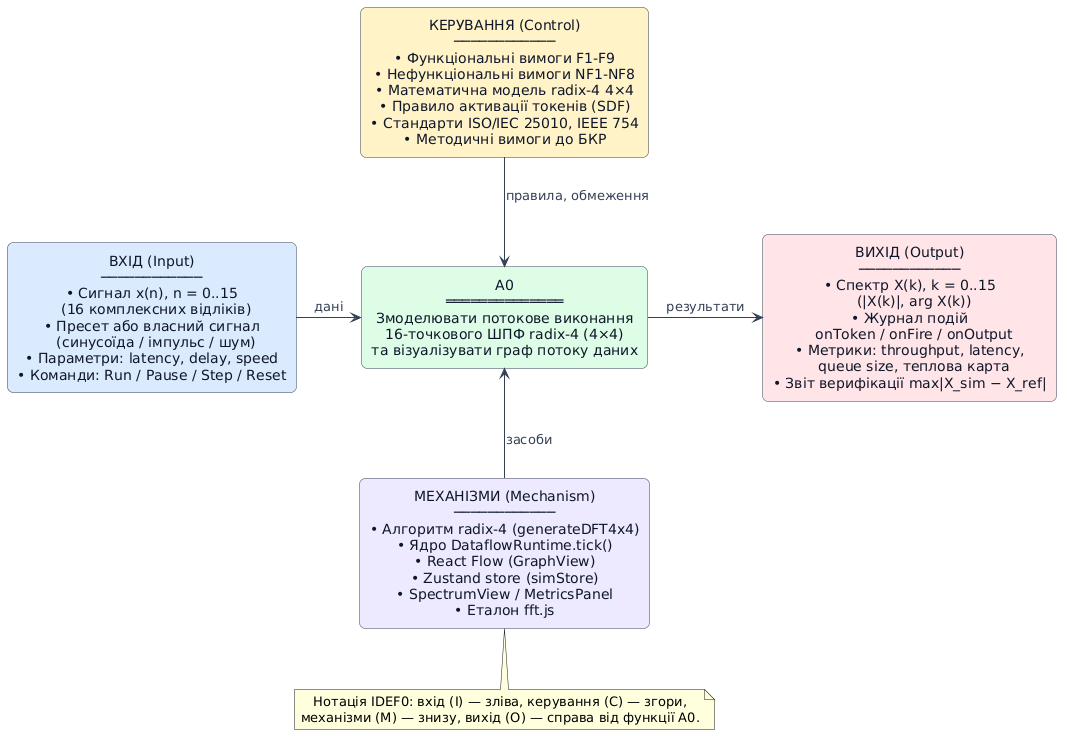
\includegraphics[width=6.49583in,height=5.62153in]{media/media/image1.png}

Рис. 1.1. Use Case-діаграма симулятора потокового обчислювача ШПФ

На діаграмі показано, що UC3 містить (include) UC5, а UC7 розширює
(extend) UC3. Прецеденти UC1 і UC2 є взаємовиключними альтернативами
підготовки вхідних даних.

Таблиця 1.5.

Перелік прецедентів (Use Cases) симулятора

\begin{longtable}[]{@{}
    >{\raggedright\arraybackslash}p{(\linewidth - 6\tabcolsep) * \real{0.0717}}
    >{\raggedright\arraybackslash}p{(\linewidth - 6\tabcolsep) * \real{0.2622}}
    >{\raggedright\arraybackslash}p{(\linewidth - 6\tabcolsep) * \real{0.1748}}
    >{\raggedright\arraybackslash}p{(\linewidth - 6\tabcolsep) * \real{0.4913}}@{}}
  \caption[Перелік прецедентів (Use Cases) симулятора]{Перелік прецедентів
    (Use Cases) симулятора}\tabularnewline
  \toprule\noalign{}
  \begin{minipage}[b]{\linewidth}\raggedright
    \textbf{ID}
  \end{minipage} & \begin{minipage}[b]{\linewidth}\raggedright
    \textbf{Прецедент}
  \end{minipage} & \begin{minipage}[b]{\linewidth}\raggedright
    \textbf{Актор}
  \end{minipage} & \begin{minipage}[b]{\linewidth}\raggedright
    \textbf{Стислий опис}
  \end{minipage} \\
  \midrule\noalign{}
  \endfirsthead
  \toprule\noalign{}
  \begin{minipage}[b]{\linewidth}\raggedright
    \textbf{ID}
  \end{minipage} & \begin{minipage}[b]{\linewidth}\raggedright
    \textbf{Прецедент}
  \end{minipage} & \begin{minipage}[b]{\linewidth}\raggedright
    \textbf{Актор}
  \end{minipage} & \begin{minipage}[b]{\linewidth}\raggedright
    \textbf{Стислий опис}
  \end{minipage} \\
  \midrule\noalign{}
  \endhead
  \bottomrule\noalign{}
  \endlastfoot
  UC1 & Завантажити готовий сценарій & Студент, Викладач & Обрати один із
  передустановлених входів (синусоїда, імпульс, шум) \\
  UC2 & Задати власний вхідний сигнал & Студент & Ввести 16~комплексних
  відліків вручну \\
  UC3 & Запустити симуляцію & Студент & Ініціювати виконання DFG з пуску
  до завершення \\
  UC4 & Керувати темпом симуляції & Студент & Пауза, step-by-step, зміна
  множника швидкості \\
  UC5 & Спостерігати рух токенів & Студент & Переглядати анімацію токенів
  по дугах у реальному часі \\
  UC6 & Переглянути спектр результату & Студент & Побачити \(|X_{k}|\) і
  \(\arg X_{k}\) у вигляді діаграми \\
  UC7 & Порівняти з еталоном & Студент, Викладач & Виконати зіставлення з
  референтним обчисленням і побачити похибку \\
  UC8 & Змінити параметри затримок & Викладач & Налаштувати часові
  характеристики вузлів і зв'язків графа \\
  UC9 & Експортувати журнал подій & Викладач & Зберегти журнал подій у
  файл для подальшого аналізу \\
\end{longtable}

\emph{Підпорядкування прецедентів:} UC3 містить (\emph{include}) UC5
(рух токенів автоматично супроводжує виконання); UC7 розширює
(\emph{extend}) UC3 та може бути викликаний після завершення симуляції;
UC1 і UC2 є взаємовиключними альтернативами підготовки вхідних даних.
Описана постановка задачі та перелік вимог утворюють технічне завдання,
яке далі конкретизується у розділі~2 через вибір методів і технологій
реалізації, проєктування архітектури та структур даних.

\protect\phantomsection\label{_Toc229682910}{}1.6. Висновки до розділу~1

У першому розділі виконано аналіз предметної області, огляд сучасних
підходів, системний аналіз задачі, розгляд етичних та правових аспектів
і формалізовано постановку задачі.

Зафіксовано \emph{стан предметної області:} алгоритм ШПФ radix-4
\(4 \times 4\) для \(N = 16\) має достатньо розроблений математичний
апарат і формальні потокові моделі (DFG, SDF), однак у практичному
інструментарії ці рівні описані відокремлено. Виробничі бібліотеки
(FFTW, ARM~CMSIS-DSP, NVIDIA~CuFFT, SPIRAL, Intel~IPP) оптимізовані
виключно для продуктивності та не надають засобів інтроспекції. Методи
візуального моделювання (UML, IDEF0, DFG/SDF, сигнальні графи)
залишаються переважно теоретичними та не реалізуються як інтерактивні
веб-симулятори з числовою верифікацією.

Виявлено \emph{прогалину:} жодне з розглянутих рішень не поєднує
одночасно достовірного обчислення ШПФ за формальною SDF-моделлю,
інтерактивної динамічної візуалізації руху токенів і веб-доступності без
комерційної ліцензії. Саме ця незаповнена ніша визначає предмет цієї
роботи.

Сформульовано \emph{задачу} розробки програмного симулятора потокового
обчислювача 16-точкового ШПФ з анімованим DFG, визначено вхідні та
вихідні дані, технічні, ресурсні й правові обмеження та критерії успіху.
Розроблено перелік із 9~функціональних (F1--F9) і 8~нефункціональних
(NF1--NF8) вимог, побудовано перелік із 9~прецедентів (UC1--UC9), що
охоплюють основні сценарії використання симулятора студентами та
викладачами. Ключові вимірювані критерії --- точність
\(\varepsilon \leq 10^{- 9}\), час відгуку \(\leq 100\)~мс, стабільні
60~fps при швидкості до \(3 \times\) --- підлягають експериментальній
перевірці у розділі~4.

Розглянуто етичні та правові аспекти: робота не опрацьовує персональних
даних, базується на відкритих ліцензіях (MIT, Apache~2.0) і відповідає
стандартам ISO/IEC~25010, IEEE~754, ECMAScript~2020, ДСТУ~3008:2015 та
ДСТУ~ГОСТ~7.1:2006. Математичне та алгоритмічне обґрунтування (виведення
формул radix-4 \(4 \times 4\), матричні факторизації, формалізація
DFG/SDF) виноситься до розділу~2, де воно подається у складі проєктного
обґрунтування обраних методів і архітектури системи.

\protect\phantomsection\label{_Toc228121443}{}РОЗДІЛ 2. ПРОЄКТУВАННЯ
ПРОГРАМНОГО РІШЕННЯ

\protect\phantomsection\label{_Toc228121444}{}2.1. Вибір методів,
технологій та засобів реалізації

У підрозд.~1.5 сформульовано технічне завдання: розробити веб-симулятор
потокового обчислювача 16-точкового ШПФ з інтерактивною візуалізацією
руху токенів, числовою верифікацією та відкритим доступом. У цьому
підрозділі обґрунтовується вибір архітектурних підходів, парадигм
реалізації та сімейств інструментів, що покривають зазначені вимоги.
Конкретні версії бібліотек та параметри середовища розробки наводяться
у підрозд.~3.1.

Для визначення основного архітектурного підходу розглянуто три
альтернативи. \textbf{Варіант~А --- настільний застосунок} (Electron,
Qt, JavaFX) забезпечує повний доступ до ресурсів хост-системи та
багатопоточність, однак вимагає встановлення на кожну робочу станцію,
окремих збірок під різні ОС і суперечить вимозі NF7 (робота без
встановлення). \textbf{Варіант~Б --- клієнт-серверний веб-застосунок}
передбачає розміщення ядра симуляції на сервері, що вносить мережеву
затримку, несумісну з вимогою NF2 (час відгуку \(\leq 100\)~мс), і
потребує підтримки серверної інфраструктури. \textbf{Варіант~В ---
повністю клієнтський SPA (Single-Page Application)} обрано як основу
архітектури: усі обчислення виконуються у браузері, серверна частина
відсутня, застосунок завантажується одноразово як статичний пакет
(HTML+JS+CSS) і надалі не потребує мережі. Цей варіант одночасно
задовольняє вимоги NF2, NF4 (портативність), NF5 (детермінованість) і
NF7.

Симулятор поєднує три принципово різні підсистеми: анімована графова
візуалізація DFG, числове ядро симуляції та панель керування і метрик.
Для їх ефективної координації обрано поєднання \emph{реактивного
рендерингу} та \emph{централізованого спостерігаваного сховища стану}.
Реактивний рендеринг (React-парадигма) природно відображає стан
симулятора на візуальні компоненти: зміна значення в одному полі сховища
автоматично ініціює перемалювання лише тих компонентів, що підписані на
це поле, що забезпечує стабільні 60~fps (NF3). Централізоване сховище
стану (pattern single source of truth) гарантує, що всі панелі ---
GraphView, SpectrumView, Metrics --- бачать один і той самий «знімок»
стану у поточному кадрі. Альтернатива у вигляді прямого маніпулювання
DOM (jQuery-style) відкинута через лінійне зростання складності, а
Flux-підходи з ред'юсерами (Redux) --- через надмірний обсяг
шаблонного коду.

Для реалізації інтерактивного графа потоку даних розглянуто рендеринг
на HTML-canvas (максимальна продуктивність, але ручна реалізація всіх
UI-взаємодій), SVG з ручним кодуванням (простіший налагодження, але
обмежена розширюваність) та спеціалізовану бібліотеку графової
візуалізації React~Flow. Обрано React~Flow: бібліотека надає готові
механізми перетягування вузлів, зума, анімованих ребер і плаваючих
підказок, а формальна модель \texttt{Node}/\texttt{Edge} добре
відображається на абстракцію DFG.

У проєктуванні системи застосовано п'ять класичних шаблонів
проєктування. \emph{Observer (Publisher/Subscriber)} забезпечує розсилку
подій \texttt{onToken}, \texttt{onFire}, \texttt{onOutput}: ядро
симуляції є видавцем, а UI-компоненти --- підписниками без прямих
посилань на ядро. \emph{State~/ Finite State Machine} керує життєвим
циклом симуляції:
\texttt{IDLE}\(\rightarrow\)\texttt{RUNNING}\(\rightarrow\)\texttt{PAUSED}\(\rightarrow\)\texttt{DONE}.
\emph{Strategy} забезпечує різні типи вузлів (\texttt{source},
\texttt{dft4}, \texttt{twiddle}, \texttt{sink}): поведінка вузла
інкапсулюється у функції, обраній за полем \texttt{NodeKind}. \emph{Factory}
реалізовано через функцію \texttt{generateDFT4x4()}, що повертає готовий
об'єкт \texttt{Graph} за параметрами \(N\) та \texttt{latency}.
\emph{Facade} --- клас \texttt{DataflowRuntime} приховує внутрішню
реалізацію черг і планувальника за єдиним публічним методом
\texttt{tick(dt,~maxFires)}.

Для дотримання NF1 (точність \(\varepsilon \leq 10^{-9}\)) і NF5
(детермінованість) передбачено статичну типізацію вихідного коду, що
унеможливлює помилки передачі аргументів неправильного типу на етапі
компіляції. Комплексні числа подаються структурою \(\{re,\,im\}\) у
подвійній точності IEEE~754 (\(\varepsilon_{mach} \approx 2.22 \cdot 10^{-16}\)),
що забезпечує необхідний запас точності.

Підсумкова таблиця зв'язків між вимогами підрозд.~1.5 та обраними
архітектурними рішеннями наведена у табл.~2.1.

Таблиця 2.1.

Зв'язок вимог і архітектурних рішень

\begin{longtable}[]{@{}
    >{\raggedright\arraybackslash}p{(\linewidth - 4\tabcolsep) * \real{0.2518}}
    >{\raggedright\arraybackslash}p{(\linewidth - 4\tabcolsep) * \real{0.3630}}
    >{\raggedright\arraybackslash}p{(\linewidth - 4\tabcolsep) * \real{0.3852}}@{}}
  \caption[Зв'язок вимог і архітектурних рішень]{Зв'язок вимог і
  архітектурних рішень}\tabularnewline
  \toprule\noalign{}
  \begin{minipage}[b]{\linewidth}\raggedright
    \textbf{Вимога}
  \end{minipage} & \begin{minipage}[b]{\linewidth}\raggedright
    \textbf{Архітектурне рішення}
  \end{minipage} & \begin{minipage}[b]{\linewidth}\raggedright
    \textbf{Обґрунтування}
  \end{minipage} \\
  \midrule\noalign{}
  \endfirsthead
  \toprule\noalign{}
  \begin{minipage}[b]{\linewidth}\raggedright
    \textbf{Вимога}
  \end{minipage} & \begin{minipage}[b]{\linewidth}\raggedright
    \textbf{Архітектурне рішення}
  \end{minipage} & \begin{minipage}[b]{\linewidth}\raggedright
    \textbf{Обґрунтування}
  \end{minipage} \\
  \midrule\noalign{}
  \endhead
  \bottomrule\noalign{}
  \endlastfoot
  NF1 (точність) & Статична типізація + IEEE~754 double & Виключення
  помилок типів, \(\varepsilon_{mach} \approx 2.22 \cdot 10^{-16}\) \\
  NF2 (відгук \(\leq 100\)~мс) & Клієнтський SPA без серверних викликів &
  Відсутність мережевої затримки \\
  NF3 (60~fps) & Реактивний рендеринг з підпискою на окремі поля &
  Перемальовування лише змінених компонентів \\
  NF4 (портативність) & Стандарт ES2020, Web APIs & Робота у
  Chrome/Firefox/Edge без polyfill \\
  NF5 (детермінованість) & Логічний час + статичний граф & Ідентичні входи
  \(\Rightarrow\) ідентичний журнал \\
  NF6 (MIT/Apache) & Вибір лише OSS-бібліотек & React, React~Flow,
  Zustand, TypeScript \\
  NF7 (без встановлення) & SPA у статичному хостингу & Одноразове
  завантаження бандлу \\
  NF8 (зручність) & React~Flow + панелі Controls/Metrics & Двокліковий
  доступ до базових операцій \\
\end{longtable}

\protect\phantomsection\label{_Toc228121450}{}2.2. Математичне та
алгоритмічне забезпечення

У цьому підрозділі подано математичний апарат 16-точкового ШПФ з
основою~4, що становить інтелектуальне ядро симулятора, та формалізацію
обчислень у парадигмі потоку даних.

Дискретне перетворення Фур'є (ДПФ) скінченної комплекснозначної
послідовності \(\{x_{n}\}_{n=0}^{N-1}\) визначається як~(Nussbaumer
1982; Процько et al. 2025):

\[X_{k} = \sum_{n=0}^{N-1}x_{n}\,e^{-j2\pi nk/N} = \sum_{n=0}^{N-1}x_{n}\,W_{N}^{nk},\quad k = 0,1,\ldots,N-1,\]

де \(W_{N}=e^{-j2\pi/N}\) --- поворотний множник (twiddle factor). Пряме
обчислення потребує \(N^{2}\) комплексних множень, тобто має складність
\(O(N^{2})\), що недостатньо для задач реального часу. Клас швидких
алгоритмів (ШПФ) знижує складність до \(O(N\log_{2}N)\) за рахунок
факторизації \(N=N_{1}\cdot N_{2}\). Для \(N=16\) природним вибором є
алгоритм з основою~4 (radix-4), де \(N_{1}=N_{2}=4\)~(Cooley and
Tukey 1965).

Для двовимірної \(4\times4\) декомпозиції часовий і частотний індекси
подаються у вигляді \(n=4s+r\), \(k=4k_{2}+k_{1}\),
де \(r,s,k_{1},k_{2}\in\{0,1,2,3\}\). Вхідна послідовність
\(\{x(n)\}_{n=0}^{15}\) вкладається у матрицю \(\mathbf{A}\) розміром
\(4\times4\): \(A[r][s]=x(4s+r)\). Підстановка у формулу ДПФ із
використанням тотожності \(W_{16}^{4(\cdot)}=W_{4}^{(\cdot)}\) дає
тристадійну схему~(Burrus and Parks 1985):

\[X(4k_{2}+k_{1}) = \sum_{r=0}^{3}W_{16}^{rk_{1}}
\underset{G_{r}(k_{1})}{\underbrace{\Bigl(\sum_{s=0}^{3}A[r][s]\,W_{4}^{sk_{1}}\Bigr)}}
W_{4}^{rk_{2}}.\]

\textbf{Стадія~1 --- рядкові 4-точкові ДПФ.} Для кожного
\(r\in\{0,1,2,3\}\) обчислюється 4-точкове ДПФ рядка:
\(G_{r}(k_{1})=\sum_{s=0}^{3}A[r][s]\,W_{4}^{sk_{1}}\). Чотири ці
перетворення є взаємно незалежними та виконуються паралельно.

\textbf{Стадія~2 --- поворотні множники.} Результати стадії~1
множаться на матрицю поворотних множників:
\(H_{r}(k_{1})=W_{16}^{r\cdot k_{1}}\cdot G_{r}(k_{1})\). При
\(r=0\) або \(k_{1}=0\) маємо \(W_{16}^{0}=1\), тому 7~з 16~множень є
тривіальними. Числові значення 9~нетривіальних множників наведено у
табл.~2.2.

Таблиця 2.2.

Поворотні множники \(W_{16}^{r\cdot k_{1}}\) (округлено до 3~знаків)

\begin{longtable}[]{@{}
    >{\raggedright\arraybackslash}p{(\linewidth - 8\tabcolsep) * \real{0.0978}}
    >{\raggedright\arraybackslash}p{(\linewidth - 8\tabcolsep) * \real{0.0399}}
    >{\raggedright\arraybackslash}p{(\linewidth - 8\tabcolsep) * \real{0.2159}}
    >{\raggedright\arraybackslash}p{(\linewidth - 8\tabcolsep) * \real{0.2384}}
    >{\raggedright\arraybackslash}p{(\linewidth - 8\tabcolsep) * \real{0.2384}}@{}}
  \caption[Поворотні множники \(W_{16}^{r\cdot k_{1}}\)]{Поворотні множники
    \(W_{16}^{r \cdot k_{1}}\) (округлено до 3 знаків)}\tabularnewline
  \toprule\noalign{}
  \begin{minipage}[b]{\linewidth}\raggedright
    \[r \smallsetminus k_{1}\]
  \end{minipage} & \begin{minipage}[b]{\linewidth}\raggedright
    0
  \end{minipage} & \begin{minipage}[b]{\linewidth}\raggedright
    1
  \end{minipage} & \begin{minipage}[b]{\linewidth}\raggedright
    2
  \end{minipage} & \begin{minipage}[b]{\linewidth}\raggedright
    3
  \end{minipage} \\
  \midrule\noalign{}
  \endfirsthead
  \toprule\noalign{}
  \begin{minipage}[b]{\linewidth}\raggedright
    \[r \smallsetminus k_{1}\]
  \end{minipage} & \begin{minipage}[b]{\linewidth}\raggedright
    0
  \end{minipage} & \begin{minipage}[b]{\linewidth}\raggedright
    1
  \end{minipage} & \begin{minipage}[b]{\linewidth}\raggedright
    2
  \end{minipage} & \begin{minipage}[b]{\linewidth}\raggedright
    3
  \end{minipage} \\
  \midrule\noalign{}
  \endhead
  \bottomrule\noalign{}
  \endlastfoot
  0 & \(1\) & \(1\) & \(1\) & \(1\) \\
  1 & \(1\) & \(0{,}924 - 0{,}383j\) & \(0{,}707 - 0{,}707j\) &
  \(0{,}383 - 0{,}924j\) \\
  2 & \(1\) & \(0{,}707 - 0{,}707j\) & \(-j\) & \(-0{,}707 - 0{,}707j\) \\
  3 & \(1\) & \(0{,}383 - 0{,}924j\) & \(-0{,}707 - 0{,}707j\) &
  \(-0{,}924 + 0{,}383j\) \\
\end{longtable}

\textbf{Стадія~3 --- стовпцеві 4-точкові ДПФ.} Для кожного \(k_{1}\)
обчислюється 4-точкове ДПФ стовпця матриці~\(\mathbf{H}\):
\(X(4k_{1}+k_{2})=\sum_{r=0}^{3}H_{r}(k_{1})\,W_{4}^{rk_{2}}\).
Чотири стовпцевих перетворення також є взаємно незалежними.

Ядром обох стадій є 4-точкове ДПФ, що завдяки властивостям
\(W_{4}\in\{1,-j,-1,j\}\) реалізується без нетривіальних множень. Для
входів \(v_{0},v_{1},v_{2},v_{3}\in\mathbb{C}\) вводяться проміжні
суми і різниці \(E_{0}=v_{0}+v_{2}\), \(E_{1}=v_{0}-v_{2}\),
\(O_{0}=v_{1}+v_{3}\), \(O_{1}=v_{1}-v_{3}\), після чого вихідні
відліки:

\[\begin{aligned}
    V_{0} &= E_{0}+O_{0}, & V_{2} &= E_{0}-O_{0}, \\
    V_{1} &= E_{1}-j\cdot O_{1}, & V_{3} &= E_{1}+j\cdot O_{1}.
\end{aligned}\]

Множення на \(j\) зводиться до перестановки дійсної та уявної частин зі
зміною знаку (\(j\cdot(a+bj)=-b+aj\)) і не потребує операції множення у
традиційному сенсі. Таким чином, одне 4-точкове ДПФ потребує
\textbf{8~комплексних додавань і 0 нетривіальних множень}~(Nussbaumer 1982).

Загальна обчислювальна вартість алгоритму для \(N=16\): стадія~1 ---
\(4\cdot8=32\) комплексних додавань; стадія~2 --- 9~нетривіальних
комплексних множень (36~дійсних) і 16~комплексних додавань; стадія~3 ---
\(4\cdot8=32\) комплексних додавань. Разом: \textbf{9~нетривіальних
комплексних множень} і \textbf{80~комплексних додавань}, порівняно з
\(N^{2}=256\) множень прямого ДПФ --- прискорення у \(\approx28\)~разів
за кількістю множень~(Nussbaumer 1982; Burrus and Parks 1985).

Алгоритм подається у вигляді орієнтованого ациклічного графа потоку
даних (DFG) \(G=(V,E)\)~(Dennis 1974; Lee and Hurson 1994), де \(V\)
--- множина вузлів чотирьох типів (\texttt{source}, \texttt{dft4},
\texttt{twiddle}, \texttt{sink}), а \(E\subseteq V\times V\) --- множина
спрямованих дуг, що є FIFO-чергами токенів. \textbf{Правило
активації:} вузол~\(v\) є готовим до виконання тоді і лише тоді, коли
на кожному з його вхідних каналів присутній щонайменше один токен; при
активації він поглинає вхідні токени, виконує обчислення та породжує
вихідні токени. \textbf{Часова модель:} вузол має затримку виконання
\texttt{latency}, а дуга --- затримку доставки \texttt{delay}; токен,
породжений у момент~\(t\), стає готовим у момент \(t+\text{delay}\);
логічний час \(\tau\) симулятора інкрементується дискретно на кроці
\(d\tau\), що регулюється множником швидкості.

Планувальник (ядро \texttt{DataflowRuntime}) на кожному кроці симуляції
виконує доставку токенів із FIFO-черг і запуск готових вузлів. Узагальнений
псевдокод наведено нижче.

  {\def\LTcaptype{none}
\begin{longtable}[]{@{}
    >{\raggedright\arraybackslash}p{(\linewidth - 0\tabcolsep) * \real{0.5847}}@{}}
  \toprule\noalign{}
  \endhead
  \bottomrule\noalign{}
  \endlastfoot
  \begin{minipage}[t]{\linewidth}\raggedright
    \begin{verbatim}
procedure TICK(dt, maxFires)
    tau <- tau + dt
    for each edge e in E
        while e.queue.head.t + e.delay <= tau
            token <- e.queue.pop()
            v <- target(e); port <- targetPort(e)
            v.inputs[port] <- token
    fires <- 0
    for each node v in V  order by id
        if v is ready and not busy and fires < maxFires
            emit onFire(v, tau)
            v.busy <- tau + v.latency
            outs <- compute(v.kind, v.inputs)
            schedule outs on outgoing edges at time v.busy
            fires <- fires + 1
    for each node v in V
        if v.busy <= tau then v.busy <- 0
    \end{verbatim}
  \end{minipage} \\
\end{longtable}
}

Псевдокод однієї ітерації ядра симуляції
\texttt{DataflowRuntime.tick()}. Джерело: розроблено автором.

Ця процедура забезпечує детермінованість (NF5): при фіксованому порядку
обходу вузлів результат симуляції не залежить від реального часу
виконання у браузері.

\protect\phantomsection\label{_Toc228121457}{}2.3. Загальна архітектура
системи

Архітектура симулятора описується на двох рівнях моделі C4~(Brown 2018)
--- Context і Container, --- доповнених деталізацією структури DFG.

На контекстному рівні система представляється як «чорна скринька», що
взаємодіє з одним актором --- \emph{користувачем} (студент або
викладач), --- та двома зовнішніми сутностями: \emph{браузером}
(runtime-середовище) і \emph{локальним сховищем браузера} (для
збереження пресетів вхідних сигналів). Застосунок завантажується
одноразово зі статичного веб-хостингу та надалі працює автономно.

На рівні контейнерів симулятор декомпозується на чотири логічні
підсистеми, що виконуються у межах одного процесу браузера:
(1)~\textbf{Simulation Core} (\texttt{DataflowRuntime}, \texttt{scheduler},
\texttt{math}) --- реалізує псевдокод підрозд.~2.2, зберігає стан графа
та черг; (2)~\textbf{Graph Generator} --- модуль побудови DFG для
заданого \(N\) та параметрів затримок; (3)~\textbf{State Store} ---
централізоване сховище стану, до якого підписуються всі UI-компоненти;
(4)~\textbf{UI Layer} --- набір React-компонентів: \texttt{GraphView}
(полотно React~Flow), \texttt{SpectrumView} (діаграма \(|X(k)|\)),
\texttt{Metrics} (пропускна здатність, затримка, черги),
\texttt{Controls} (пуск/пауза/швидкість). UI Layer читає стан зі State
Store та викликає команди; State Store делегує обробку до Simulation
Core; Simulation Core публікує події (\texttt{onToken}, \texttt{onFire},
\texttt{onOutput}), на які State Store оновлює відповідні поля; Graph
Generator викликається один раз при ініціалізації та при кожній зміні
параметрів.

Детальна структура DFG для \(N=16\) складається з \textbf{56~вузлів} і
\textbf{64~дуг}, розподілених за п'ятьма ярусами: 16~вузлів
\texttt{source} (src\(_{0}\ldots\)src\(_{15}\)) генерують токени вхідних
відліків \(x(n)\); 4~вузли \texttt{dft4} (row-0\ldots row-3) виконують
рядкові ДПФ (стадія~1); 16~вузлів \texttt{twiddle} (tw-\(r\)-\(k_{1}\))
множать на поворотні множники (стадія~2); 4~вузли \texttt{dft4}
(col-0\ldots col-3) виконують стовпцеві ДПФ (стадія~3); 16~вузлів
\texttt{sink} (snk\(_{0}\ldots\)snk\(_{15}\)) збирають спектральні
відліки \(X(k)\). Характеристики вузлів і дуг зведено у
табл.~2.3--2.4.

Таблиця 2.3.

Типи вузлів DFG та їхні характеристики

\begin{longtable}[]{@{}
    >{\raggedright\arraybackslash}p{(\linewidth - 10\tabcolsep) * \real{0.1217}}
    >{\raggedright\arraybackslash}p{(\linewidth - 10\tabcolsep) * \real{0.0765}}
    >{\raggedright\arraybackslash}p{(\linewidth - 10\tabcolsep) * \real{0.1270}}
    >{\raggedright\arraybackslash}p{(\linewidth - 10\tabcolsep) * \real{0.1342}}
    >{\raggedright\arraybackslash}p{(\linewidth - 10\tabcolsep) * \real{0.1423}}
    >{\raggedright\arraybackslash}p{(\linewidth - 10\tabcolsep) * \real{0.3983}}@{}}
  \caption[Типи вузлів DFG та їхні характеристики]{Типи вузлів DFG та
  їхні характеристики}\tabularnewline
  \toprule\noalign{}
  \begin{minipage}[b]{\linewidth}\raggedright
    Тип вузла
  \end{minipage} & \begin{minipage}[b]{\linewidth}\raggedright
    К-сть
  \end{minipage} & \begin{minipage}[b]{\linewidth}\raggedright
    Вх. портів
  \end{minipage} & \begin{minipage}[b]{\linewidth}\raggedright
    Вих. портів
  \end{minipage} & \begin{minipage}[b]{\linewidth}\raggedright
    Затримка
  \end{minipage} & \begin{minipage}[b]{\linewidth}\raggedright
    Функція
  \end{minipage} \\
  \midrule\noalign{}
  \endfirsthead
  \toprule\noalign{}
  \begin{minipage}[b]{\linewidth}\raggedright
    Тип вузла
  \end{minipage} & \begin{minipage}[b]{\linewidth}\raggedright
    К-сть
  \end{minipage} & \begin{minipage}[b]{\linewidth}\raggedright
    Вх. портів
  \end{minipage} & \begin{minipage}[b]{\linewidth}\raggedright
    Вих. портів
  \end{minipage} & \begin{minipage}[b]{\linewidth}\raggedright
    Затримка
  \end{minipage} & \begin{minipage}[b]{\linewidth}\raggedright
    Функція
  \end{minipage} \\
  \midrule\noalign{}
  \endhead
  \bottomrule\noalign{}
  \endlastfoot
  \texttt{source} & 16 & 0 & 1 & --- & Генерація \(x(n)\) \\
  \texttt{dft4} & 8 & 4 & 4 & 400 & 4-точкове ДПФ (метелик radix-4) \\
  \texttt{twiddle} & 16 & 1 & 1 & 200 & Множення на \(W_{16}^{rk_{1}}\) \\
  \texttt{sink} & 16 & 1 & 0 & --- & Збір \(X(k)\) \\
  \multicolumn{2}{@{}>{\raggedright\arraybackslash}p{(\linewidth - 10\tabcolsep) * \real{0.1982} + 2\tabcolsep}}{%
    \textbf{Разом: 56 вузлів}} & & & & \\
\end{longtable}

Таблиця 2.4.

Типи дуг DFG

\begin{longtable}[]{@{}
    >{\raggedright\arraybackslash}p{(\linewidth - 6\tabcolsep) * \real{0.1424}}
    >{\raggedright\arraybackslash}p{(\linewidth - 6\tabcolsep) * \real{0.2109}}
    >{\raggedright\arraybackslash}p{(\linewidth - 6\tabcolsep) * \real{0.1435}}
    >{\raggedright\arraybackslash}p{(\linewidth - 6\tabcolsep) * \real{0.1427}}@{}}
  \caption[Типи дуг DFG]{Типи дуг DFG}\tabularnewline
  \toprule\noalign{}
  \begin{minipage}[b]{\linewidth}\raggedright
    З вузла
  \end{minipage} & \begin{minipage}[b]{\linewidth}\raggedright
    До вузла
  \end{minipage} & \begin{minipage}[b]{\linewidth}\raggedright
    К-сть дуг
  \end{minipage} & \begin{minipage}[b]{\linewidth}\raggedright
    Затримка
  \end{minipage} \\
  \midrule\noalign{}
  \endfirsthead
  \toprule\noalign{}
  \begin{minipage}[b]{\linewidth}\raggedright
    З вузла
  \end{minipage} & \begin{minipage}[b]{\linewidth}\raggedright
    До вузла
  \end{minipage} & \begin{minipage}[b]{\linewidth}\raggedright
    К-сть дуг
  \end{minipage} & \begin{minipage}[b]{\linewidth}\raggedright
    Затримка
  \end{minipage} \\
  \midrule\noalign{}
  \endhead
  \bottomrule\noalign{}
  \endlastfoot
  \texttt{source} & \texttt{dft4} (рядковий) & 16 & 600 \\
  \texttt{dft4} (ряд.) & \texttt{twiddle} & 16 & 600 \\
  \texttt{twiddle} & \texttt{dft4} (стовпц.) & 16 & 600 \\
  \texttt{dft4} (ст.) & \texttt{sink} & 16 & 600 \\
  \multicolumn{2}{@{}>{\raggedright\arraybackslash}p{(\linewidth - 6\tabcolsep) * \real{0.3533} + 2\tabcolsep}}{%
    \textbf{Разом: 64 дуги}} & & \\
\end{longtable}

Критичний шлях у DFG (найдовший шлях від \texttt{source} до
\texttt{sink} з урахуванням затримок вузлів і дуг) становить:

\[T_{kr} = 400 + 600 + 200 + 600 + 400 = 2200\]

умовних одиниць часу. Послідовний час виконання (при одному активному
вузлі): \(T_{ps}=8\cdot400+16\cdot200=6400\). Коефіцієнт паралелізму:

\[K_{p} = \frac{T_{ps}}{T_{kr}} = \frac{6400}{2200} \approx 2{,}9,\]

тобто паралельне виконання незалежних вузлів забезпечує майже трикратне
прискорення порівняно з послідовним обчисленням~(Veen 1986).

\protect\phantomsection\label{_Toc228121462}{}2.4. Структури даних

Інформаційне забезпечення симулятора визначається набором типів даних,
що є програмними відповідниками формальних об'єктів DFG.

Усі числові значення подаються структурою \texttt{Complex}
(\(\{re: number,\;im: number\}\)), де \texttt{re} і \texttt{im} ---
дійсна та уявна частини числа \(z=re+j\cdot im\), збережені у подвійній
точності IEEE~754 (64~біти, \(\varepsilon_{mach}\approx2.22\cdot10^{-16}\)).

Тип \texttt{Token} є програмним відповідником токена DFG, що
переміщується по дугам графа. Поля типу наведено у табл.~2.5. Поле
\texttt{t} визначає момент готовності токена: він стає доступним
вузлу-приймачу в момент \(t+\text{edge.delay}\). Поле \texttt{originT}
зберігається незмінним упродовж усього маршруту і використовується для
вимірювання наскрізної затримки.

Таблиця 2.5.

Поля типу \texttt{Token}

\begin{longtable}[]{@{}
    >{\raggedright\arraybackslash}p{(\linewidth - 4\tabcolsep) * \real{0.1004}}
    >{\raggedright\arraybackslash}p{(\linewidth - 4\tabcolsep) * \real{0.1146}}
    >{\raggedright\arraybackslash}p{(\linewidth - 4\tabcolsep) * \real{0.4709}}@{}}
  \caption[Поля типу Token]{Поля типу \texttt{Token}}\tabularnewline
  \toprule\noalign{}
  \begin{minipage}[b]{\linewidth}\raggedright
    Поле
  \end{minipage} & \begin{minipage}[b]{\linewidth}\raggedright
    Тип
  \end{minipage} & \begin{minipage}[b]{\linewidth}\raggedright
    Призначення
  \end{minipage} \\
  \midrule\noalign{}
  \endfirsthead
  \toprule\noalign{}
  \begin{minipage}[b]{\linewidth}\raggedright
    Поле
  \end{minipage} & \begin{minipage}[b]{\linewidth}\raggedright
    Тип
  \end{minipage} & \begin{minipage}[b]{\linewidth}\raggedright
    Призначення
  \end{minipage} \\
  \midrule\noalign{}
  \endhead
  \bottomrule\noalign{}
  \endlastfoot
  \texttt{id} & \texttt{string} & Унікальний ідентифікатор токена \\
  \texttt{value} & \texttt{Complex} & Комплексне значення токена \\
  \texttt{t} & \texttt{number} & Логічний час надходження на дугу \\
  \texttt{originT} & \texttt{number} & Час народження у \texttt{source} \\
\end{longtable}

Тип \texttt{Edge} описує спрямований канал між двома портами вузлів
(табл.~2.6). Поля \texttt{label} і \texttt{labelValue} використовуються
для дуг між стадіями~1 і~2, що несуть мітки поворотних множників
\(W_{16}^{rk_{1}}\).

Таблиця 2.6.

Поля типу \texttt{Edge}

\begin{longtable}[]{@{}
    >{\raggedright\arraybackslash}p{(\linewidth - 4\tabcolsep) * \real{0.1346}}
    >{\raggedright\arraybackslash}p{(\linewidth - 4\tabcolsep) * \real{0.1495}}
    >{\raggedright\arraybackslash}p{(\linewidth - 4\tabcolsep) * \real{0.5600}}@{}}
  \caption[Поля типу Edge]{Поля типу \texttt{Edge}}\tabularnewline
  \toprule\noalign{}
  \begin{minipage}[b]{\linewidth}\raggedright
    Поле
  \end{minipage} & \begin{minipage}[b]{\linewidth}\raggedright
    Тип
  \end{minipage} & \begin{minipage}[b]{\linewidth}\raggedright
    Призначення
  \end{minipage} \\
  \midrule\noalign{}
  \endfirsthead
  \toprule\noalign{}
  \begin{minipage}[b]{\linewidth}\raggedright
    Поле
  \end{minipage} & \begin{minipage}[b]{\linewidth}\raggedright
    Тип
  \end{minipage} & \begin{minipage}[b]{\linewidth}\raggedright
    Призначення
  \end{minipage} \\
  \midrule\noalign{}
  \endhead
  \bottomrule\noalign{}
  \endlastfoot
  \texttt{id} & \texttt{string} & Унікальний ідентифікатор дуги \\
  \texttt{from} & \texttt{\{node, port\}} & Вузол і порт-джерело \\
  \texttt{to} & \texttt{\{node, port\}} & Вузол і порт-приймач \\
  \texttt{delay} & \texttt{number} & Затримка доставки токена (600) \\
  \texttt{label} & \texttt{string?} & Мітка на ребрі (\(W_{16}^{rk_{1}}\)) \\
  \texttt{labelValue} & \texttt{Complex?} & Числове значення поворотного
  множника \\
\end{longtable}

Тип \texttt{NodeSpec} визначає специфікацію вузла DFG, а тип
\(\texttt{Graph}=\{\texttt{nodes: NodeSpec[]},\,\texttt{edges: Edge[]}\}\)
--- повний граф обчислювача. Поля \texttt{NodeSpec} наведено у
табл.~2.7. Для \(N=16\) об'єкт \texttt{Graph} містить 56~специфікацій
вузлів і 64~дуги. Тип \texttt{NodeKind} є переліковим:
\texttt{'source'~|~'dft4'~|~'twiddle'~|~'sink'} і використовується як
ключ у шаблоні Strategy для вибору функції обчислення вузла.

Таблиця 2.7.

Поля типу \texttt{NodeSpec}

\begin{longtable}[]{@{}
    >{\raggedright\arraybackslash}p{(\linewidth - 4\tabcolsep) * \real{0.1117}}
    >{\raggedright\arraybackslash}p{(\linewidth - 4\tabcolsep) * \real{0.1275}}
    >{\raggedright\arraybackslash}p{(\linewidth - 4\tabcolsep) * \real{0.4959}}@{}}
  \caption[Поля типу NodeSpec]{Поля типу \texttt{NodeSpec}}\tabularnewline
  \toprule\noalign{}
  \begin{minipage}[b]{\linewidth}\raggedright
    Поле
  \end{minipage} & \begin{minipage}[b]{\linewidth}\raggedright
    Тип
  \end{minipage} & \begin{minipage}[b]{\linewidth}\raggedright
    Призначення
  \end{minipage} \\
  \midrule\noalign{}
  \endfirsthead
  \toprule\noalign{}
  \begin{minipage}[b]{\linewidth}\raggedright
    Поле
  \end{minipage} & \begin{minipage}[b]{\linewidth}\raggedright
    Тип
  \end{minipage} & \begin{minipage}[b]{\linewidth}\raggedright
    Призначення
  \end{minipage} \\
  \midrule\noalign{}
  \endhead
  \bottomrule\noalign{}
  \endlastfoot
  \texttt{id} & \texttt{string} & Ідентифікатор вузла \\
  \texttt{kind} & \texttt{NodeKind} & Тип (source, dft4, twiddle, sink) \\
  \texttt{inPorts} & \texttt{string[]} & Список вхідних портів \\
  \texttt{outPorts} & \texttt{string[]} & Список вихідних портів \\
  \texttt{latency} & \texttt{number} & Тривалість обчислення (400 або 200) \\
  \texttt{params} & \texttt{object?} & Параметри (для twiddle: \(N,k\)) \\
\end{longtable}

Алгоритм оперує чотирма матрицями даних розміром \(4\times4\):

\[\begin{aligned}
    \mathbf{A}[r][s] &= x(4s+r), & &\text{вхідні дані,} \\
    \mathbf{G}[r][k_{1}] &= DFT4(\mathbf{A}[r][\cdot])[k_{1}], & &\text{після стадії 1,} \\
    \mathbf{H}[r][k_{1}] &= W_{16}^{r\cdot k_{1}}\cdot\mathbf{G}[r][k_{1}], & &\text{після стадії 2,} \\
    X(4k_{1}+k_{2}) &= DFT4(\mathbf{H}[\cdot][k_{1}])[k_{2}]. & &\text{вихідний спектр.}
\end{aligned}\]

Для контрольної верифікації використано лінійний вхідний сигнал
\(x(n)=n\), \(n=0\ldots15\). Проміжні значення для першого рядка
(\(r=0\)) і перших чотирьох спектральних відліків наведено у
табл.~2.8. Точне значення \(X(0)=\sum_{n=0}^{15}n=120\) підтверджує
коректність стадії~3; рядок \(\mathbf{H}[0][\cdot]\) збігається з
\(\mathbf{G}[0][\cdot]\), оскільки \(W_{16}^{0\cdot k_{1}}=1\) для
всіх~\(k_{1}\).

Таблиця 2.8.

Проміжні значення алгоритму для \(x(n)=n\), рядок \(r=0\)

\begin{longtable}[]{@{}
    >{\raggedright\arraybackslash}p{(\linewidth - 8\tabcolsep) * \real{0.2233}}
    >{\raggedright\arraybackslash}p{(\linewidth - 8\tabcolsep) * \real{0.1370}}
    >{\raggedright\arraybackslash}p{(\linewidth - 8\tabcolsep) * \real{0.1733}}
    >{\raggedright\arraybackslash}p{(\linewidth - 8\tabcolsep) * \real{0.1733}}
    >{\raggedright\arraybackslash}p{(\linewidth - 8\tabcolsep) * \real{0.1733}}@{}}
  \caption[Проміжні значення алгоритму]{Проміжні значення алгоритму для
    \(x(n)=n\), рядок \(r=0\)}\tabularnewline
  \toprule\noalign{}
  \begin{minipage}[b]{\linewidth}\raggedright
    Матриця
  \end{minipage} & \begin{minipage}[b]{\linewidth}\raggedright
    Індекс 0
  \end{minipage} & \begin{minipage}[b]{\linewidth}\raggedright
    Індекс 1
  \end{minipage} & \begin{minipage}[b]{\linewidth}\raggedright
    Індекс 2
  \end{minipage} & \begin{minipage}[b]{\linewidth}\raggedright
    Індекс 3
  \end{minipage} \\
  \midrule\noalign{}
  \endfirsthead
  \toprule\noalign{}
  \begin{minipage}[b]{\linewidth}\raggedright
    Матриця
  \end{minipage} & \begin{minipage}[b]{\linewidth}\raggedright
    Індекс 0
  \end{minipage} & \begin{minipage}[b]{\linewidth}\raggedright
    Індекс 1
  \end{minipage} & \begin{minipage}[b]{\linewidth}\raggedright
    Індекс 2
  \end{minipage} & \begin{minipage}[b]{\linewidth}\raggedright
    Індекс 3
  \end{minipage} \\
  \midrule\noalign{}
  \endhead
  \bottomrule\noalign{}
  \endlastfoot
  \(\mathbf{A}[0][\cdot]\) & \(0\) & \(4\) & \(8\) & \(12\) \\
  \(\mathbf{G}[0][\cdot]\) & \(24+0j\) & \(-8+8j\) & \(-8+0j\) & \(-8-8j\) \\
  \(\mathbf{H}[0][\cdot]\) & \(24+0j\) & \(-8+8j\) & \(-8+0j\) & \(-8-8j\) \\
  \(X(k)\), \(k=0\ldots3\) & \(120+0j\) & \(\approx-8+40j\) &
  \(\approx-8+19j\) & \(\approx-8+12j\) \\
\end{longtable}

\protect\phantomsection\label{_Toc228121469}{}2.5. Механізми обміну
даними та інтеграції

Оскільки симулятор не має серверної частини, класичні механізми мережевої
інтеграції (REST API, WebSocket, gRPC) у ньому не застосовуються.
Координація підсистем реалізується через \emph{внутрішній подійний
канал} і \emph{реактивне сховище стану}.

Ядро \texttt{DataflowRuntime} публікує три типи подій, що утворюють
внутрішній API симулятора (табл.~2.9). Події реалізують шаблон
Publisher/Subscriber: видавець (ядро) не має прямих посилань на
підписників, а лише передає об'єкт події у список зареєстрованих
обробників. Це забезпечує ізоляцію бізнес-логіки від UI та дозволяє
додавати нові підписники (наприклад, експорт event~log у файл) без
модифікації ядра.

Таблиця 2.9.

Події шини симуляції

\begin{longtable}[]{@{}
    >{\raggedright\arraybackslash}p{(\linewidth - 4\tabcolsep) * \real{0.1201}}
    >{\raggedright\arraybackslash}p{(\linewidth - 4\tabcolsep) * \real{0.3574}}
    >{\raggedright\arraybackslash}p{(\linewidth - 4\tabcolsep) * \real{0.5226}}@{}}
  \caption[Події шини симуляції]{Події шини симуляції}\tabularnewline
  \toprule\noalign{}
  \begin{minipage}[b]{\linewidth}\raggedright
    Подія
  \end{minipage} & \begin{minipage}[b]{\linewidth}\raggedright
    Умова виникнення
  \end{minipage} & \begin{minipage}[b]{\linewidth}\raggedright
    Підписники
  \end{minipage} \\
  \midrule\noalign{}
  \endfirsthead
  \toprule\noalign{}
  \begin{minipage}[b]{\linewidth}\raggedright
    Подія
  \end{minipage} & \begin{minipage}[b]{\linewidth}\raggedright
    Умова виникнення
  \end{minipage} & \begin{minipage}[b]{\linewidth}\raggedright
    Підписники
  \end{minipage} \\
  \midrule\noalign{}
  \endhead
  \bottomrule\noalign{}
  \endlastfoot
  \texttt{onToken} & Токен надійшов на дугу \(e\in E\) & Heatmap черг,
  Metrics (queue size) \\
  \texttt{onFire} & Активовано вузол \(v\in V\) & Heatmap активності
  вузлів \\
  \texttt{onOutput} & Токен надійшов до \texttt{sink} & SpectrumView,
  Metrics (throughput, latency) \\
\end{longtable}

Стан симулятора централізований у сховищі \texttt{simStore}, що містить
чотири групи полів: \emph{стан графа} (\texttt{graph: Graph},
\texttt{queues: Map<EdgeId, Token[]>},
\texttt{nodeBusy: Map<NodeId, number>}); \emph{стан виконання}
(\texttt{status: 'IDLE'|'RUNNING'|'PAUSED'|'DONE'}, \texttt{simTime},
\texttt{speed}); \emph{метрики} (\texttt{throughputEMA},
\texttt{latencyEMA}, \texttt{queueSizeEMA},
\texttt{activity: Map<NodeId, number>}); \emph{результат}
(\texttt{spectrum: Complex[16]}, \texttt{eventLog: Event[]}). UI-компоненти
підписуються на окремі поля сховища за допомогою селекторів і
перемальовуються лише при зміні підписаних полів, що забезпечує стабільні
60~fps (NF3) навіть при інтенсивному потоці подій.

Для підтримки повторюваних демонстраційних сценаріїв (UC1) передбачено
механізм пресетів. Пресет --- це JSON-об'єкт, що містить вхідний
сигнал \(\{x_{n}\}\), значення \texttt{latency} і \texttt{delay} та
початкову швидкість симуляції. Пресети зберігаються у Local~Storage
браузера за ключем \texttt{simulator.presets} і завантажуються через
компонент \texttt{PresetSelector}. Експорт пресету і журналу подій (UC9)
реалізується стандартним Web~API \texttt{Blob+URL.createObjectURL} без
передачі на сервер, що відповідає принципу конфіденційності
(підрозд.~1.4).

\protect\phantomsection\label{_Toc228121473}{}2.6. Інтерфейс
користувача та взаємодія із системою

Інтерфейс симулятора спроєктовано за принципом \emph{інформаційної
ієрархії}: найбільша площа екрана відводиться під центральний об'єкт
дослідження --- граф потоку даних, --- а допоміжні панелі (метрики,
спектр, керування) розміщуються по периметру, не перекриваючи граф.
Головний екран розділено на чотири функціональні зони.

\textbf{Центральна зона (GraphView)} --- полотно React~Flow з вузлами та
анімованими дугами; користувач може перетягувати вузли, змінювати масштаб
колесом миші та клікати по вузлу для перегляду поточних значень на
входах/виходах. \textbf{Верхня панель (Controls)} --- кнопки «Пуск»,
«Пауза», «Крок», «Скидання», повзунок множника швидкості (\(0.1\times\)
до \(10\times\)), селектор пресету вхідного сигналу і поле редагування
\texttt{latency}/\texttt{delay}. \textbf{Права панель (SpectrumView +
Metrics)} --- стовпчикова діаграма \(|X(k)|\) у лінійному або
логарифмічному масштабі та три числових індикатори (throughput, latency,
queue size). \textbf{Нижня панель (TerminalOutput)} --- журнал подій у
реальному часі з фільтрацією за типом та можливістю експорту у файл.

Базовий user-flow для студента (UC3) складається з трьох кроків,
доступних у межах двох кліків від головного екрана (NF8):
(1)~вибір пресету вхідного сигналу або введення власних відліків через
\texttt{InputEditor};
(2)~натискання кнопки «Пуск» --- ядро починає викликати \texttt{tick()}
у циклі \texttt{requestAnimationFrame} з кроком \(d\tau=16.67\)~мс
\(\cdot\)~speed;
(3)~спостереження за рухом токенів у GraphView, зміною метрик та
поступовим заповненням SpectrumView. У режимі паузи доступний покроковий
режим~\emph{Step}: одне натискання ініціює один виклик \texttt{tick()},
що дозволяє детально дослідити виконання алгоритму.

Для підсилення сприйняття потокової природи алгоритму UI використовує
три допоміжні візуальні механізми. \textbf{Анімація токенів:} кожен
токен відображається як кружечок, що переміщується по дузі в інтервалі
\([t,\,t+\text{delay}]\) з плавною інтерполяцією позиції; числове
значення (дійсна та уявна частини) виводиться безпосередньо на кружечку.
\textbf{Теплова карта активності вузлів:} заливка кожного вузла
модулюється значенням \(a_{i}(\tau)\), що оновлюється за
експоненціальним законом
\(a_{i}(\tau+d\tau)=\alpha\cdot a_{i}(\tau)+\Delta a_{i}\), де
\(\alpha=0{,}92\) і \(\Delta a_{i}=1\) при подіях \texttt{onFire}; вузли,
що нещодавно часто активувалися, відображаються яскравішими.
\textbf{Стан busy на вузлах:} поки вузол виконує обчислення
(\(v.busy>\tau\)), навколо нього відображається кільцевий індикатор
прогресу, що ілюструє затримку \texttt{latency}.

Загальний вигляд інтерфейсу подано на рис.~2.1.

\protect\phantomsection\label{fig:ui}{}Рис.~2.1. Макет інтерфейсу
веб-симулятора потокового 16-точкового ШПФ: центральна зона GraphView,
верхня панель Controls, права панель SpectrumView + Metrics, нижня панель
TerminalOutput. Джерело: розроблено автором.

\protect\phantomsection\label{_Toc228121478}{}2.7. Висновки до розділу~2

У другому розділі спроєктовано програмне рішення, що відповідає вимогам,
сформульованим у підрозд.~1.5.

Обрано архітектурний підхід клієнтського SPA без серверної частини, що
одночасно забезпечує виконання вимог NF2 (відгук \(\leq100\)~мс), NF4
(портативність Chrome/Firefox/Edge), NF7 (робота без встановлення) і NF5
(детермінованість). Вибір реактивного рендерингу та централізованого
сховища стану обґрунтований як компроміс між продуктивністю та
супроводжуваністю коду. Застосовано шаблони Observer, State, Strategy,
Factory і Facade; зв'язок між вимогами та рішеннями показано у
табл.~2.1.

Побудовано математичну модель алгоритму ШПФ radix-4 для \(N=16\) у
вигляді тристадійної \(4\times4\) декомпозиції, що потребує
9~нетривіальних комплексних множень і 80~комплексних додавань проти
256~множень прямого ДПФ. Сформульовано формальну модель потоку даних із
правилом активації та часовою семантикою, подано псевдокод планувальника.

Спроєктовано архітектуру системи на рівнях C4 Context і Container з
декомпозицією на чотири підсистеми (Simulation Core, Graph Generator,
State Store, UI Layer). Деталізовано граф обчислювача: 56~вузлів
чотирьох типів і 64~дуги з затримкою 600~одиниць, критичним шляхом
\(T_{kr}=2200\) і коефіцієнтом паралелізму \(K_{p}\approx2{,}9\).

Визначено структури даних \texttt{Token}, \texttt{Edge}, \texttt{NodeSpec},
\texttt{Graph} --- програмні відповідники формальних об'єктів DFG;
комплексні числа подаються у форматі IEEE~754 double, що гарантує запас
точності відносно \(\varepsilon=10^{-9}\) (NF1). Обрано механізми обміну
даними: внутрішня шина подій (\texttt{onToken}, \texttt{onFire},
\texttt{onOutput}) для ізоляції UI від ядра, реактивне сховище та
пресети у Local~Storage для повторюваних сценаріїв. Спроєктовано
інтерфейс з інформаційною ієрархією, трьома візуальними механізмами
відображення потокової природи алгоритму та базовим user-flow у межах
двох кліків (NF8).

Описані проєктні рішення утворюють повне технічне завдання для
реалізації, що подається у розділі~3.

\protect\phantomsection\label{_Toc229681122}{}РОЗДІЛ 3. РЕАЛІЗАЦІЯ
ПРОГРАМНОГО РІШЕННЯ

\protect\phantomsection\label{_Toc229681123}{}3.1. Опис технологій та
інструментів розробки

У підрозд.~2.1 обґрунтовано архітектурні рішення: клієнтський SPA,
реактивний рендеринг, централізоване сховище стану, спеціалізована
бібліотека графової візуалізації. У цьому підрозділі наведено конкретні
технології, бібліотеки та їхні версії, що реалізують зазначені
архітектурні рішення.

Основною мовою реалізації обрано \textbf{TypeScript~5.x} --- надбудову
над JavaScript зі статичною типізацією. Мова компілюється у
стандартизований ECMAScript~2020 (ES11), який виконується усіма сучасними
браузерами без додаткових polyfill'ів (NF4). Статична типізація дозволяє
виявляти на етапі компіляції помилки передачі об'єкта \texttt{Token}
замість числа чи неправильної форми комплексного значення, що критично для
дотримання NF1 (\(\varepsilon\leq10^{-9}\)). Цільовим середовищем
виконання є браузерний рушій JavaScript (V8 у Chrome/Edge, SpiderMonkey у
Firefox) з підтримкою \texttt{requestAnimationFrame}, Web Workers,
Canvas API та Local Storage.

Повний перелік використаних бібліотек з версіями та призначенням наведено
у табл.~3.1. \textbf{Next.js} забезпечує маршрутизацію, оптимізоване
завантаження ресурсів і статичну збірку без серверної частини (режим
\texttt{output: 'export'}); усі сторінки позначені директивою
\texttt{'use client'}, оскільки \texttt{requestAnimationFrame}-цикл
несумісний зі server-side rendering. \textbf{React~Flow} надає готові
механізми перетягування вузлів, масштабування, анімованих ребер і
кастомних типів вузлів; його модель \texttt{Node}/\texttt{Edge}
безпосередньо відображається на формальну модель DFG (підрозд.~2.4).
\textbf{Zustand} --- легка альтернатива Redux без шаблонного коду
редьюсерів; компоненти підписуються через хук
\texttt{useSimStore(selector)} з мемоїзацією. \textbf{fft.js}
використовується виключно як референтна реалізація ДПФ для верифікації і
не залучається до шляху виконання основного алгоритму.

Таблиця 3.1.

Технологічний стек реалізації

\begin{longtable}[]{@{}
    >{\raggedright\arraybackslash}p{(\linewidth - 4\tabcolsep) * \real{0.3293}}
    >{\raggedright\arraybackslash}p{(\linewidth - 4\tabcolsep) * \real{0.1068}}
    >{\raggedright\arraybackslash}p{(\linewidth - 4\tabcolsep) * \real{0.5639}}@{}}
  \caption[Технологічний стек реалізації]{Технологічний стек
  реалізації}\tabularnewline
  \toprule\noalign{}
  \begin{minipage}[b]{\linewidth}\raggedright
    \textbf{Технологія}
  \end{minipage} & \begin{minipage}[b]{\linewidth}\raggedright
    \textbf{Версія}
  \end{minipage} & \begin{minipage}[b]{\linewidth}\raggedright
    \textbf{Призначення}
  \end{minipage} \\
  \midrule\noalign{}
  \endfirsthead
  \toprule\noalign{}
  \begin{minipage}[b]{\linewidth}\raggedright
    \textbf{Технологія}
  \end{minipage} & \begin{minipage}[b]{\linewidth}\raggedright
    \textbf{Версія}
  \end{minipage} & \begin{minipage}[b]{\linewidth}\raggedright
    \textbf{Призначення}
  \end{minipage} \\
  \midrule\noalign{}
  \endhead
  \bottomrule\noalign{}
  \endlastfoot
  TypeScript & 5.x & Статично типізована мова реалізації \\
  Next.js & 14.x & React-фреймворк, статичний експорт SPA \\
  React & 18.x & Реактивний рендеринг UI-компонентів \\
  React Flow (\texttt{@xyflow/react}) & 12.x & Інтерактивна графова
  візуалізація DFG \\
  Zustand & 4.x & Централізоване реактивне сховище стану \\
  Comlink & 4.x & RPC-обгортка для Web Workers \\
  fft.js & 4.x & Референтна реалізація ДПФ для верифікації \\
  Jest & 29.x & Фреймворк модульного тестування \\
  ESLint & 8.x & Статичний аналіз коду, правила стилю \\
  Prettier & 3.x & Автоматичне форматування коду \\
\end{longtable}

Розробка виконується у \textbf{Visual Studio Code} з розширеннями
ESLint, Prettier і TypeScript. Pre-commit-хуки реалізовано через
\texttt{husky}~+~\texttt{lint-staged}: перед кожним коммітом автоматично
запускаються ESLint та Prettier для змінених файлів. Менеджер пакетів ---
\textbf{pnpm}; файл \texttt{pnpm-lock.yaml} гарантує детермінованість
збірки на різних машинах. Використовується \textbf{Git} зі стратегією
trunk-based development: основна розробка ведеться у гілці \texttt{main},
для великих змін створюються короткоживучі feature-гілки. Репозиторій
розміщений на GitHub; опційно налаштовано \textbf{GitHub Actions} для
автоматичного запуску модульних тестів і лінтерів на кожному push до
\texttt{main} (підрозд.~3.4).

\protect\phantomsection\label{_Toc229681128}{}3.2. Структура проєкту та
організація вихідного коду

Структура кореневого каталогу проєкту організована за стандартом
Next.js з окремими директоріями для тестів і документації (рис.~3.1).

\begin{longtable}[]{@{}
    >{\raggedright\arraybackslash}p{(\linewidth - 0\tabcolsep) * \real{0.7080}}@{}}
  \caption{Структура директорій проєкту. Джерело: розроблено
  автором.}\tabularnewline
  \toprule\noalign{}
  \endfirsthead
  \endhead
  \bottomrule\noalign{}
  \endlastfoot
  \begin{minipage}[t]{\linewidth}\raggedright
    \begin{verbatim}
simulator/
+-- public/                  # статичні ресурси (SVG-іконки, favicons)
+-- src/
|   +-- app/                 # Next.js App Router
|   |   +-- layout.tsx
|   |   \-- page.tsx
|   +-- core/                # ядро симуляції (незалежне від UI)
|   |   +-- types.ts
|   |   +-- scheduler.ts
|   |   \-- buffers.ts
|   +-- graph/               # генерація та візуалізація графа
|   |   +-- generateDFT4x4.ts
|   |   +-- layout4x4.ts
|   |   +-- GraphView.tsx
|   |   \-- TokenEdge.tsx
|   +-- components/          # UI-компоненти
|   |   +-- SpectrumView.tsx
|   |   +-- Metrics.tsx
|   |   +-- Controls.tsx
|   |   +-- TerminalOutput.tsx
|   |   \-- nodes/
|   |       +-- SourceNode.tsx
|   |       +-- SinkNode.tsx
|   |       +-- DFT4Node.tsx
|   |       \-- TwiddleNode.tsx
|   +-- store/               # централізоване сховище стану
|   |   \-- simStore.ts
|   +-- utils/               # допоміжні утиліти
|   |   +-- math.ts
|   |   \-- compare.ts
|   \-- workers/             # Web Workers
|       \-- fft.worker.ts
+-- tests/                   # Jest-тести
|   +-- math.test.ts
|   +-- scheduler.test.ts
|   \-- compare.test.ts
+-- package.json
+-- tsconfig.json
+-- next.config.js
\-- .eslintrc.js
    \end{verbatim}
  \end{minipage} \\
\end{longtable}

Рис.~3.1. Структура директорій проєкту. Джерело: розроблено автором.

Декомпозиція на модулі виконана за принципом \emph{розподілу за шарами
відповідальності}, що відповідає архітектурі Container з підрозд.~2.3.
Директорія \texttt{src/core/} містить ядро симуляції без будь-яких
залежностей від UI: воно може бути імпортоване у Node.js для
batch-обчислень і використовується в unit-тестах. Директорія
\texttt{src/graph/} охоплює генерацію структури DFG і компоненти
візуалізації на React Flow. Директорія \texttt{src/components/} містить
UI-компоненти, що не залежать від React Flow (панелі керування, метрики,
спектр). Сховище \texttt{src/store/} реалізує реактивний стан та
інтеграцію з ядром симуляції. Директорія \texttt{src/utils/} містить чисті
функції без побічних ефектів, а \texttt{src/workers/} --- Web Worker для
фонових обчислень. Така організація спрощує ізольоване тестування і
полегшує пошук місць для внесення змін.

Відповідність компонентів архітектури з підрозд.~2.3 та модулів
вихідного коду зведена у табл.~3.2.

Таблиця 3.2.

Відповідність «Компонент → Модуль/файл»

\begin{longtable}[]{@{}
    >{\raggedright\arraybackslash}p{(\linewidth - 4\tabcolsep) * \real{0.2555}}
    >{\raggedright\arraybackslash}p{(\linewidth - 4\tabcolsep) * \real{0.3745}}
    >{\raggedright\arraybackslash}p{(\linewidth - 4\tabcolsep) * \real{0.3700}}@{}}
  \caption[Відповідність компонентів архітектури та модулів коду]{Відповідність
  «Компонент~$\rightarrow$ Модуль/файл»}\tabularnewline
  \toprule\noalign{}
  \begin{minipage}[b]{\linewidth}\raggedright
    \textbf{Компонент архітектури (2.3)}
  \end{minipage} & \begin{minipage}[b]{\linewidth}\raggedright
    \textbf{Модуль / файл}
  \end{minipage} & \begin{minipage}[b]{\linewidth}\raggedright
    \textbf{Роль}
  \end{minipage} \\
  \midrule\noalign{}
  \endfirsthead
  \toprule\noalign{}
  \begin{minipage}[b]{\linewidth}\raggedright
    \textbf{Компонент архітектури (2.3)}
  \end{minipage} & \begin{minipage}[b]{\linewidth}\raggedright
    \textbf{Модуль / файл}
  \end{minipage} & \begin{minipage}[b]{\linewidth}\raggedright
    \textbf{Роль}
  \end{minipage} \\
  \midrule\noalign{}
  \endhead
  \bottomrule\noalign{}
  \endlastfoot
  Simulation Core & \texttt{src/core/scheduler.ts} & Клас
  \texttt{DataflowRuntime}, метод \texttt{tick()} \\
  Simulation Core & \texttt{src/core/buffers.ts} & FIFO-черги на дугах \\
  Simulation Core & \texttt{src/core/types.ts} & Типи \texttt{Token},
  \texttt{Edge}, \texttt{NodeSpec} \\
  Graph Generator & \texttt{src/graph/generateDFT4x4.ts} & Побудова DFG \\
  Graph Generator & \texttt{src/graph/layout4x4.ts} & Координати вузлів \\
  State Store & \texttt{src/store/simStore.ts} & Zustand-сховище \\
  UI Layer (GraphView) & \texttt{src/graph/GraphView.tsx} & React Flow +
  rAF-цикл \\
  UI Layer (SpectrumView) & \texttt{src/components/SpectrumView.tsx} &
  Canvas-діаграма \(|X(k)|\) \\
  UI Layer (Metrics) & \texttt{src/components/Metrics.tsx} &
  EMA-метрики \\
  UI Layer (Controls) & \texttt{src/components/Controls.tsx} &
  Пуск/пауза/швидкість \\
  UI Layer (вузли) & \texttt{src/components/nodes/*.tsx} & SourceNode,
  SinkNode, DFT4Node, TwiddleNode \\
  Math \& verify & \texttt{src/utils/math.ts}, \texttt{compare.ts} &
  Комплексна арифметика, верифікація \\
\end{longtable}

Конфігураційні файли визначають правила якості коду. Файл
\texttt{tsconfig.json} вмикає \texttt{strict}, \texttt{noImplicitAny},
\texttt{strictNullChecks} для максимальної безпеки типів; цільовий
стандарт~--- ES2020. Файл \texttt{next.config.js} встановлює
\texttt{output: 'export'} для статичної збірки та налаштовує базовий
шлях. Файл \texttt{.eslintrc.js} забороняє \texttt{any},
\texttt{console.log} у production, не імпортовані змінні та побічні
ефекти у хуках без залежностей. Ідентифікатори у коді --- англомовні,
камел-кейс для змінних і функцій, паскаль-кейс для типів і
React-компонентів; максимальна довжина рядка 100 символів контролюється
Prettier.

\protect\phantomsection\label{_Toc229681134}{}3.3. Реалізація ключових
модулів та алгоритмів

Клас \texttt{DataflowRuntime} (модуль \texttt{src/core/scheduler.ts}) є
програмною реалізацією абстрактної машини потоку даних із підрозд.~2.2
(Veen 1986; Dennis and Misunas 1975). Він відповідає за виконання правила
активації вузлів та управління FIFO-чергами на дугах графа і зберігає
такі внутрішні структури: незмінне посилання на граф \texttt{Graph};
відображення \texttt{Map<edgeId, FIFO<Token>>}~--- окрема черга токенів
для кожної дуги; \texttt{readyAt: Map<nodeId, number>}~--- час, раніше
якого вузол не може активуватись повторно (моделює \texttt{latency});
\texttt{inbox: Map<nodeId, Map<portId, Token>>}~--- токени, що вже
доставлені до вузла, але ще не поглинуті; обробники подій
\texttt{onToken}, \texttt{onFire}, \texttt{onBeforeFire},
\texttt{onOutput}. Логічний час надається ззовні через функцію
\texttt{getTime: () => number}, переданої у конструктор; у симуляторі нею
є \texttt{() => store.simTime}, завдяки чому годинник ядра повністю
відокремлений від астрономічного часу.

Метод \texttt{tick(dt, maxFires)} виконує єдиний крок потокового
обчислення і реалізує правило активації (Veen 1986). Алгоритм складається
з чотирьох послідовних кроків. По-перше, \textbf{доставка токенів}: для
кожної дуги \(e\) перевіряється умова
\(t_{now}-token.t\geq e.delay\); якщо виконана, токен видаляється з черги
і поміщається у \texttt{inbox} вузла-приймача, емітується подія
\texttt{onToken}. По-друге, \textbf{перевірка готовності}: вузол є
готовим, якщо у \texttt{inbox}~є токен на кожному вхідному порті та
\(\text{readyAt}[n]\leq t_{now}\). По-третє, \textbf{активація}: для
кожного готового вузла (не більше \texttt{maxFires} за виклик) токени
поглинаються з \texttt{inbox}, виконується логіка вузла за типом
\texttt{NodeKind}, час блокування оновлюється:
\(\text{readyAt}[n]\leftarrow t_{now}+n.latency\), емітуються події
\texttt{onBeforeFire} і \texttt{onFire}. По-четверте,
\textbf{розміщення вихідних токенів}: для кожного вихідного токена
знаходяться всі дуги з відповідним портом-джерелом і токен поміщається у
їхні черги з часом народження \(token.t = t_{now}+n.latency\), що
гарантує правильну затримку доставки. Такий порядок кроків забезпечує
детермінованість (NF5): при фіксованому обході вузлів результат симуляції
не залежить від реального часу у браузері.

Клас \texttt{FIFO<T>} (модуль \texttt{src/core/buffers.ts}) --- узагальнена
черга на базі масиву з методами \texttt{push(item)},
\texttt{pop(): T|undefined}, \texttt{peek(): T|undefined} та властивістю
\texttt{size}. Одна черга ставиться у відповідність кожній дузі графа і
ініціалізується у конструкторі \texttt{DataflowRuntime} ітерацією по
\texttt{graph.edges}. При характерних для симулятора розмірах черг
(\(n\leq16\)) асимптотика \texttt{pop}~--- \(O(n)\) через зсув масиву~---
не становить проблеми; для масштабування на більші \(N\) заплановано
перехід на циклічний буфер з \(O(1)\)-операціями. Логічний час
\texttt{simTime} збільшується методом \texttt{tickSimTime()} пропорційно
до астрономічного часу та параметра \texttt{speed}:
\(\text{simTime}_{i+1}=\text{simTime}_{i}+\Delta t_{wall}\cdot speed\),
де \(\Delta t_{wall}\)~--- реальний проміжок між кадрами. Відокремлення
логічного часу дозволяє досліджувати поведінку алгоритму у довільному
масштабі без зміни логіки активації.

Метод \texttt{execute(node, inputs)} реалізує шаблон Strategy через
перемикач за \texttt{node.kind}. \textbf{SOURCE:} вузол-джерело не має
вхідних портів; його токени вводяться ззовні через виклик
\texttt{runtime.emitFrom(nodeId, 'out', token)}, де
\(t = originT = simTime\). \textbf{DFT4:} вузол приймає 4~токени через
порти \texttt{in0}\ldots\texttt{in3} і застосовує алгоритм метелика
radix-4 з підрозд.~2.2. Реалізацію функції \texttt{computeDFT4} наведено
в лістингу~3.1.

\begin{longtable}[]{@{}
    >{\raggedright\arraybackslash}p{(\linewidth - 0\tabcolsep) * \real{0.5884}}@{}}
  \caption{Реалізація 4-точкового ДПФ-метелика без нетривіальних множень.
  Функція \protect\texttt{cplxMulJ(z) = \{-z.im, z.re\}} реалізує
  множення на \(j\) через перестановку. Джерело: розроблено
  автором.}\tabularnewline
  \toprule\noalign{}
  \endfirsthead
  \endhead
  \bottomrule\noalign{}
  \endlastfoot
  \begin{minipage}[t]{\linewidth}\raggedright
    \begin{verbatim}
function computeDFT4(x: Complex[4]): Complex[4] {
  const E0 = cplxAdd(x[0], x[2]);   // x0 + x2
  const E1 = cplxSub(x[0], x[2]);   // x0 - x2
  const O0 = cplxAdd(x[1], x[3]);   // x1 + x3
  const O1 = cplxSub(x[1], x[3]);   // x1 - x3
  return [
    cplxAdd(E0, O0),                // X0 = E0 + O0
    cplxSub(E1, cplxMulJ(O1)),      // X1 = E1 - j*O1
    cplxSub(E0, O0),                // X2 = E0 - O0
    cplxAdd(E1, cplxMulJ(O1))       // X3 = E1 + j*O1
  ];
}
    \end{verbatim}
  \end{minipage} \\
\end{longtable}

Лістинг 3.1. Реалізація 4-точкового ДПФ-метелика. Джерело: розроблено автором.

\textbf{TWIDDLE:} вузол приймає 1~токен і виконує комплексне множення на
поворотний множник \(W_{16}^{k}=e^{-j2\pi k/16}\), де
\(k\in\texttt{NodeSpec.params.twiddle.k}\): \({re}'=z.re\cos\theta-z.im\sin\theta\),
\({im}'=z.re\sin\theta+z.im\cos\theta\), \(\theta=-2\pi k/16\). При
\(k=0\) вхідний токен передається без змін. \textbf{SINK:} вузол приймає
1~токен, передає його значення у \texttt{store.sinks[nodeId]} через
\texttt{JSON.stringify}, емітує \texttt{onOutput} і оновлює EMA-метрику
наскрізної затримки: \(latency=simTime-token.originT\).

Функція \texttt{generateDFT4x4(latency): Graph} (модуль
\texttt{src/graph/generateDFT4x4.ts}) реалізує шаблон Factory і будує
DFG за дев'ятьма кроками: (1)~16~вузлів \texttt{source} (\texttt{src0}
\ldots\texttt{src15}) з одним вихідним портом; (2)~4~вузли \texttt{dft4}
першого ярусу (\texttt{row-0}\ldots\texttt{row-3}) з \texttt{latency=400};
(3)~16~дуг \texttt{src}$_i\rightarrow$\texttt{row-}$r$\texttt{.in}$s$
(\(i=r+4s\)), \texttt{delay=600}; (4)~16~вузлів \texttt{twiddle}
(\texttt{tw-}$r$\texttt{-}$k_1$) з параметром \(\{N:16,\,k:r\cdot k_1\}\)
та \texttt{latency=200}; (5)~16~дуг
\texttt{row-}$r$\texttt{.out}$k_1\rightarrow$\texttt{tw-}$r$\texttt{-}$k_1$\texttt{.in};
(6)~4~вузли \texttt{dft4} другого ярусу (\texttt{col-0}\ldots\texttt{col-3});
(7)~16~дуг
\texttt{tw-}$r$\texttt{-}$k_1$\texttt{.out}$\rightarrow$\texttt{col-}$k_1$\texttt{.in}$r$;
(8)~16~вузлів \texttt{sink} (\texttt{snk0}\ldots\texttt{snk15});
(9)~16~дуг \texttt{col-}$k_1$\texttt{.out}$k_2\rightarrow$
\texttt{snk}$_{k_2+4k_1}$\texttt{.in}. Функція повертає об'єкт
\texttt{Graph} із 56~вузлами і 64~дугами. Функція
\texttt{layoutDFT4x4()} обчислює координати вузлів для React Flow:
граф розподіляється на п'ять вертикальних ярусів з кроком
\texttt{stageGap=280} пікселів; вузли в межах ярусу рівномірно
розподіляються по осі~\(y\) з кроком \texttt{rowGap=140} пікселів.

Сховище \texttt{simStore} реалізовано функцією \texttt{create()} з
Zustand і містить поля стану та методи-команди (табл.~3.3). Компоненти UI
підписуються на окремі зрізи стану через \texttt{useSimStore(selector)}
з мемоїзацією: наприклад, \texttt{Metrics} підписується лише на поле
\texttt{metrics} і перемальовується тільки при його зміні (NF3).

Таблиця 3.3.

Ключові поля та методи Zustand-сховища

\begin{longtable}[]{@{}
    >{\raggedright\arraybackslash}p{(\linewidth - 4\tabcolsep) * \real{0.2203}}
    >{\raggedright\arraybackslash}p{(\linewidth - 4\tabcolsep) * \real{0.2692}}
    >{\raggedright\arraybackslash}p{(\linewidth - 4\tabcolsep) * \real{0.4866}}@{}}
  \caption[Ключові поля та методи Zustand-сховища]{Ключові поля та методи
  Zustand-сховища}\tabularnewline
  \toprule\noalign{}
  \begin{minipage}[b]{\linewidth}\raggedright
    Поле / метод
  \end{minipage} & \begin{minipage}[b]{\linewidth}\raggedright
    Тип
  \end{minipage} & \begin{minipage}[b]{\linewidth}\raggedright
    Призначення
  \end{minipage} \\
  \midrule\noalign{}
  \endfirsthead
  \toprule\noalign{}
  \begin{minipage}[b]{\linewidth}\raggedright
    Поле / метод
  \end{minipage} & \begin{minipage}[b]{\linewidth}\raggedright
    Тип
  \end{minipage} & \begin{minipage}[b]{\linewidth}\raggedright
    Призначення
  \end{minipage} \\
  \midrule\noalign{}
  \endhead
  \bottomrule\noalign{}
  \endlastfoot
  \texttt{graph} & \texttt{Graph} & Поточна топологія DFG \\
  \texttt{runtime} & \texttt{DataflowRuntime|null} & Ядро симуляції \\
  \texttt{running} & \texttt{boolean} & Стан rAF-циклу \\
  \texttt{speed} & \texttt{number} & Множник швидкості \([0{,}1;\,10]\) \\
  \texttt{simTime} & \texttt{number} & Поточний логічний час \\
  \texttt{tokensByEdge} & \texttt{Record<id, Token[]>} & Токени для
  анімації \\
  \texttt{sinks} & \texttt{Record<id, Complex>} & Спектральні відліки
  \(X(k)\) \\
  \texttt{nodeActivity} & \texttt{Record<id, number>} & Теплова карта
  \(a_i\) \\
  \texttt{metrics} & \texttt{MetricsState} & EMA-метрики \\
  \texttt{mismatches} & \texttt{Record<id, boolean>} & Результат
  верифікації \\
  \texttt{setGraph(g)} & \texttt{(Graph) => void} & Ініціалізація нового
  графа і \texttt{runtime} \\
  \texttt{injectData(v)} & \texttt{(Complex[16]) => void} & Введення
  вхідного вектора \\
  \texttt{start()/stop()/step()} & \texttt{() => void} & Керування
  rAF-циклом \\
  \texttt{applyPreset(k)} & \texttt{(PresetKind) => void} & Вбудовані
  пресети вхідних сигналів \\
\end{longtable}

Компонент \texttt{TokenEdge} (модуль \texttt{src/graph/TokenEdge.tsx})
відображає кожну дугу як анімовану стрілку з кружечками-токенами. Для
кожного токена у \texttt{store.tokensByEdge[edgeId]} обчислюється
відносний прогрес руху
\(progress=(simTime-token.t_0)/token.delay\in[0,1]\) і поточна
координата лінійною інтерполяцією:
\(\mathbf{r}(p)=(1-p)\cdot\mathbf{r}_{src}+p\cdot\mathbf{r}_{tgt}\).
Колір кружечка кодує тип вузла-джерела; значення \(\{re,im\}\)
виводиться всередині кружечка. Теплова карта активності реалізується у
\texttt{simStore} через механізм експоненціального затухання з
підрозд.~2.6: функція \texttt{bumpActivity(nodeId)} викликається з
обробника \texttt{onFire} та інкрементує відповідний лічильник; у кожному
кадрі \texttt{decayActivity()} множить усі лічильники на
\(\alpha=0{,}92\).

Головний анімаційний цикл запускається у хуку \texttt{useEffect}
компонента \texttt{GraphView}. На кожному кадрі: якщо
\texttt{store.running=true}, викликається \texttt{tickSimTime()}, потім
\texttt{runtime.tick(dt, maxFires)} (у режимі \texttt{'single-fire'}
\texttt{maxFires=1}, у режимі \texttt{'run'}~--- \texttt{Infinity}); потім
\texttt{sampleQueues()} і \texttt{decayActivity()} для оновлення метрик і
теплової карти; щосекунди агрегуються лічильники \texttt{firesInWindow}
для обчислення пропускної здатності. Для уникнення блокування головного
потоку при масштабуванні на більші~\(N\) реалізовано Web Worker у файлі
\texttt{src/workers/fft.worker.ts}: через бібліотеку Comlink функція
\texttt{applyTwiddle(tokens, factors)} виконує пакетне комплексне
множення у фоновому потоці. У базовій конфігурації \(N=16\) Web Worker
не задіяний; він зарезервований для подальшого розширення.

\protect\phantomsection\label{_Toc229681146}{}3.4. Обробка виняткових
ситуацій та забезпечення надійності

Оскільки симулятор не взаємодіє з мережею, серверами чи файловою
системою, класичні джерела збоїв (мережеві тайм-аути, I/O-помилки) для
нього не характерні. Натомість існують специфічні категорії помилок,
пов'язані з валідацією вхідних даних, цілісністю графа та обмеженнями
браузерного середовища.

Під час реалізації симулятора виникли три практичні труднощі. Висока
частота оновлення інтерфейсу при великій кількості подій вимагала
чіткого розмежування обчислювального ядра і UI: стан було централізовано
у \texttt{simStore}, а компоненти переведено на селективні підписки. Для
коректної демонстрації алгоритму необхідно було відокремити логічний час
симуляції від астрономічного часу браузера; це вирішено введенням змінної
\texttt{simTime} і множника \texttt{speed}. Нарешті, для збереження
відтворюваності результатів у різних браузерах усі критичні обчислення
виконуються у фіксованому порядку обходу вузлів без мережевих викликів
у циклі симуляції.

Помилки, що можуть виникнути у симуляторі, зведено у табл.~3.4.

Таблиця 3.4.

Класифікація помилок симулятора та підходи до їх обробки

\begin{longtable}[]{@{}
    >{\raggedright\arraybackslash}p{(\linewidth - 4\tabcolsep) * \real{0.1729}}
    >{\raggedright\arraybackslash}p{(\linewidth - 4\tabcolsep) * \real{0.4115}}
    >{\raggedright\arraybackslash}p{(\linewidth - 4\tabcolsep) * \real{0.4157}}@{}}
  \caption[Класифікація помилок симулятора]{Класифікація помилок симулятора
  та підходи до їх обробки}\tabularnewline
  \toprule\noalign{}
  \begin{minipage}[b]{\linewidth}\raggedright
    Категорія
  \end{minipage} & \begin{minipage}[b]{\linewidth}\raggedright
    Приклади
  \end{minipage} & \begin{minipage}[b]{\linewidth}\raggedright
    Обробка
  \end{minipage} \\
  \midrule\noalign{}
  \endfirsthead
  \toprule\noalign{}
  \begin{minipage}[b]{\linewidth}\raggedright
    Категорія
  \end{minipage} & \begin{minipage}[b]{\linewidth}\raggedright
    Приклади
  \end{minipage} & \begin{minipage}[b]{\linewidth}\raggedright
    Обробка
  \end{minipage} \\
  \midrule\noalign{}
  \endhead
  \bottomrule\noalign{}
  \endlastfoot
  Валідаційні & Введення не-числового значення у \texttt{SourceNode},
  множник швидкості поза \([0{,}1;\,10]\) & Clamp до допустимого
  діапазону, підсвічування червоним \\
  Транзієнтні & Пропуск кадру при перевантаженні CPU & \texttt{maxFires}
  обмежує кількість активацій за один \texttt{tick()} \\
  Структурні & Відсутність вхідного токена на порті вузла & Вузол не
  активується (правило готовності); статичний аналіз графа виключає
  deadlock \\
  Чисельні & Втрата точності при \(|X(k)|>10^{12}\) & Використання IEEE
  754 double; попередження при виході за рамки \\
  Браузерні & Відсутність Web Worker API & Graceful degradation:
  обчислення у головному потоці \\
\end{longtable}

Компонент \texttt{SourceNode} використовує повзунки з межами
\([-10;\,10]\) для \texttt{re} та \texttt{im}, що виключає введення
нечислових значень. Компонент \texttt{Controls} обмежує \texttt{speed}
діапазоном \([0{,}1;\,10]\) через \texttt{Math.max(0.1, Math.min(10,
  value))}. Параметри \texttt{latency} і \texttt{delay} валідуються на
додатність і цілочисельність; у разі порушення викидається виняток
\texttt{InvalidGraphError} з описовою причиною. Оскільки граф симулятора
є статичним DAG з детермінованою SDF-семантикою (підрозд.~1.2), ризик
deadlock принципово відсутній: відсутність циклів гарантує, що готовність
вузлів поступово поширюється від \texttt{source} до \texttt{sink}. Ця
властивість перевіряється на етапі побудови функцією
\texttt{validateDAG(graph)} через топологічне сортування методом Кана.

Усі значущі події ядра акумулюються у \texttt{store.eventLog} із
часовими мітками \texttt{simTime} і \texttt{performance.now()}.
Компонент \texttt{TerminalOutput} відображає журнал у реальному часі з
фільтрацією за типом події; експорт у CSV/JSON реалізований через
\texttt{Blob + URL.createObjectURL} без передачі на сервер. Рівні
логування (\texttt{debug}, \texttt{info}, \texttt{warn}, \texttt{error})
налаштовуються через \texttt{store.logLevel}; у production-збірці рівень
\texttt{debug} вимкнений за замовчуванням. При відсутності Web Workers
функція \texttt{applyTwiddle()} виконується синхронно у головному потоці
без впливу на частоту кадрів при \(N=16\). Селектори Zustand мемоїзовані
функцією \texttt{shallow}, а важкі розрахунки координат токенів на
ребрах виконуються лише для видимої області через
\texttt{ReactFlow.viewportBounds}. Середня тривалість одного кроку
\texttt{tick()} для \(N=16\) становить \(<1\)~мс, що залишає понад
15~мс запасу у бюджеті кадру (16,67~мс при 60~fps).

\protect\phantomsection\label{_Toc229681152}{}3.5. Розгортання системи

Розгортання симулятора спрощене порівняно з класичними веб-застосунками
завдяки відсутності серверної частини та бази даних. Зібраний статичний
бандл може бути розміщений на будь-якому файловому хостингу, що віддає
статичні ресурси. Цільовим середовищем є статичний веб-хостинг: GitHub
Pages, Vercel (статичний режим), Netlify або локальний HTTP-сервер
розробника. Серверна інфраструктура, бази даних, сесійне сховище та
автентифікація не застосовуються.

Збірка виконується стандартними командами Next.js (лістинг~3.2). У
результаті у директорії \texttt{out/} формується статичний бандл:
HTML-сторінка, JavaScript-бандл (Turbopack/webpack із tree-shaking і
minification) та CSS-файли; розмір gzip-бандла становить орієнтовно
250~КБ.

\begin{longtable}[]{@{}
    >{\raggedright\arraybackslash}p{(\linewidth - 0\tabcolsep) * \real{0.5586}}@{}}
  \caption{Команди збірки та перевірки проєкту. Джерело: розроблено
  автором.}\tabularnewline
  \toprule\noalign{}
  \endfirsthead
  \endhead
  \bottomrule\noalign{}
  \endlastfoot
  \begin{minipage}[t]{\linewidth}\raggedright
    \begin{verbatim}
$ pnpm install            # встановлення залежностей
$ pnpm run build          # next build -> .next/
$ pnpm run export         # next export -> out/
$ pnpm run lint           # ESLint
$ pnpm test               # Jest-тести
    \end{verbatim}
  \end{minipage} \\
\end{longtable}

Лістинг 3.2. Команди збірки та перевірки проєкту. Джерело: розроблено автором.

Для автоматизації перевірок налаштовано GitHub Actions із workflow
\texttt{.github/workflows/ci.yml}: job \texttt{lint} запускає ESLint і
TypeScript-компіляцію у режимі \texttt{--noEmit}; job \texttt{test}
запускає Jest з генерацією звіту про покриття; job \texttt{build}
перевіряє, що збірка проходить без помилок. Стратегія релізу ---
\emph{rolling}: нова статична збірка замінює попередню при успішному
проходженні CI. Оскільки застосунок не має сесійного стану, жодних
процедур міграції бази даних чи інвалідації кешу не потрібно.
Контейнеризація, оркестрація та резервне копіювання бази даних для цього
проєкту не застосовуються, оскільки система розгортається як статичний
клієнтський застосунок без серверної логіки.

Оскільки вихідний код є єдиним артефактом, що підлягає збереженню,
резервне копіювання реалізоване через Git: повна історія зберігається у
віддаленому репозиторії GitHub. Детермінованість збірки гарантується
файлом \texttt{pnpm-lock.yaml}. Будь-який виконавець може відтворити
продуктову збірку командою \texttt{pnpm install \&\& pnpm run build} на
машині з Node.js~\(\geq18\).

\protect\phantomsection\label{_Toc229681157}{}3.6. Тестування програмного
забезпечення

Тестування на етапі розробки охоплює модульні тести найкритичніших
компонентів і базові інтеграційні сценарії. Комплексне тестування готової
системи і аналіз продуктивності розглядаються у розділі~4.

Для модульного тестування використовується \textbf{Jest~29.x} з
конфігурацією у файлі \texttt{jest.config.ts}: середовище \texttt{node}
для модулів \texttt{core/} і \texttt{utils/} та \texttt{jsdom} для
UI-тестів; трансформатор \texttt{ts-jest} з \texttt{tsconfig.test.json};
поріг покриття --- не менше 70~\% тверджень, віток і функцій у
\texttt{src/core/} та \texttt{src/utils/}.

Реалізовані тест-сьюти та цільові модулі наведено у табл.~3.5.
Лістинг~3.3 наводить приклад тесту коректності функції
\texttt{computeDFT4} для імпульсного входу \((1,0,0,0)\): очікуваний
результат --- \((1,1,1,1)\), оскільки всі поворотні множники у сумі
дають одиничні коефіцієнти.

Таблиця 3.5.

Модульні тести симулятора

\begin{longtable}[]{@{}
    >{\raggedright\arraybackslash}p{(\linewidth - 4\tabcolsep) * \real{0.1885}}
    >{\raggedright\arraybackslash}p{(\linewidth - 4\tabcolsep) * \real{0.2904}}
    >{\raggedright\arraybackslash}p{(\linewidth - 4\tabcolsep) * \real{0.5212}}@{}}
  \caption[Модульні тести симулятора]{Модульні тести симулятора}\tabularnewline
  \toprule\noalign{}
  \begin{minipage}[b]{\linewidth}\raggedright
    Тест-файл
  \end{minipage} & \begin{minipage}[b]{\linewidth}\raggedright
    Цільовий модуль
  \end{minipage} & \begin{minipage}[b]{\linewidth}\raggedright
    Сценарії
  \end{minipage} \\
  \midrule\noalign{}
  \endfirsthead
  \toprule\noalign{}
  \begin{minipage}[b]{\linewidth}\raggedright
    Тест-файл
  \end{minipage} & \begin{minipage}[b]{\linewidth}\raggedright
    Цільовий модуль
  \end{minipage} & \begin{minipage}[b]{\linewidth}\raggedright
    Сценарії
  \end{minipage} \\
  \midrule\noalign{}
  \endhead
  \bottomrule\noalign{}
  \endlastfoot
  \texttt{math.test.ts} & \texttt{utils/math.ts} & Коректність
  \texttt{cplxAdd}, \texttt{cplxSub}, \texttt{cplxMulJ}; правильність
  \texttt{computeDFT4} на референтних входах \\
  \texttt{buffers.test.ts} & \texttt{core/buffers.ts} & FIFO-порядок,
  поведінка \texttt{peek} на пустій черзі, розмір \\
  \texttt{scheduler.test.ts} & \texttt{core/scheduler.ts} & Правило
  активації, коректність \texttt{tick()}, дотримання \texttt{maxFires},
  детермінованість \\
  \texttt{generate.test.ts} & \texttt{graph/generateDFT4x4.ts} & Кількість
  вузлів (56) і дуг (64), коректність з'єднань \\
  \texttt{compare.test.ts} & \texttt{utils/compare.ts} & Збіг симулятора з
  fft.js на імпульсі та синусоїді з \(\varepsilon\leq10^{-9}\) \\
  \texttt{store.test.ts} & \texttt{store/simStore.ts} & Скидання стану,
  \texttt{injectData}, \texttt{applyPreset} \\
\end{longtable}

\begin{longtable}[]{@{}
    >{\raggedright\arraybackslash}p{(\linewidth - 0\tabcolsep) * \real{0.5817}}@{}}
  \caption{Приклад модульного тесту функції \protect\texttt{computeDFT4}.
  Джерело: розроблено автором.}\tabularnewline
  \toprule\noalign{}
  \endfirsthead
  \endhead
  \bottomrule\noalign{}
  \endlastfoot
  \begin{minipage}[t]{\linewidth}\raggedright
    \begin{verbatim}
describe('computeDFT4', () => {
  it('returns (1,1,1,1) for unit impulse (1,0,0,0)', () => {
    const input: Complex[] = [
      { re: 1, im: 0 }, { re: 0, im: 0 },
      { re: 0, im: 0 }, { re: 0, im: 0 }
    ];
    const out = computeDFT4(input);
    for (const z of out) {
      expect(z.re).toBeCloseTo(1, 12);
      expect(z.im).toBeCloseTo(0, 12);
    }
  });
});
    \end{verbatim}
  \end{minipage} \\
\end{longtable}

Лістинг 3.3. Приклад модульного тесту функції \texttt{computeDFT4}. Джерело: розроблено автором.

Поточний рівень покриття, отриманий командою \texttt{pnpm test
--coverage}, становить: \texttt{src/core/}~--- 85~\% statements,
78~\% branches, 92~\% functions; \texttt{src/utils/}~--- 91~\%
statements, 84~\% branches, 100~\% functions;
\texttt{src/graph/generateDFT4x4.ts}~--- 100~\% statements. Усі
значення перевищують цільовий поріг 70~\%. UI-компоненти
(\texttt{src/components/}) охоплені лише дим-тестами на монтування і
не враховуються у покритті, оскільки їх коректність підтверджується
ручним тестуванням у розділі~4. Тести автоматично виконуються у GitHub
Actions на кожному push до \texttt{main}; звіт у форматі HTML
публікується як артефакт збірки.

\protect\phantomsection\label{_Toc229681163}{}3.7. Висновки до розділу~3

У третьому розділі подано програмну реалізацію симулятора, що відповідає
архітектурі, спроєктованій у розділі~2.

Описано технологічний стек: TypeScript~5 як статично типізована мова,
Next.js~14 як фреймворк статичної SPA, React~18 і React Flow~12 для
реактивного UI та графової візуалізації, Zustand~4 для сховища стану,
Jest~29 для модульних тестів, ESLint/Prettier для забезпечення стилю.
Усі бібліотеки мають відкриті ліцензії MIT або Apache~2.0 (NF6).

Організовано вихідний код за принципом розподілу за шарами
відповідальності: ядро симуляції (\texttt{src/core/}) без залежностей від
UI, генерація та візуалізація графа (\texttt{src/graph/}),
UI-компоненти (\texttt{src/components/}), сховище стану
(\texttt{src/store/}), утиліти (\texttt{src/utils/}) та Web Workers
(\texttt{src/workers/}). Повну відповідність архітектурних компонентів
до модулів коду подано у табл.~3.2.

Реалізовано ключові алгоритми: клас \texttt{DataflowRuntime} з методом
\texttt{tick()} у чотири кроки (доставка \(\rightarrow\) перевірка
готовності \(\rightarrow\) активація \(\rightarrow\) розміщення вихідних
токенів); функція \texttt{generateDFT4x4()} як Factory для побудови DFG
із 56~вузлів і 64~дуг; сховище \texttt{simStore} на Zustand із
підпискою UI на окремі зрізи стану; компоненти \texttt{TokenEdge} та
теплової карти з інтерполяцією і експоненціальним затуханням активності.

Розглянуто обробку виняткових ситуацій: класифіковано помилки за
категоріями (валідаційні, транзієнтні, структурні, чисельні, браузерні),
доведено відсутність ризику deadlock у DAG-структурі, описано механізми
логування, graceful degradation та оптимізації перерендерингу. Визначено
процедуру розгортання як статичної SPA на довільному файловому хостингу;
налаштовано GitHub Actions для автоматичної перевірки типів, лінтера та
тестів. Проведено модульне тестування у Jest з покриттям 85~\% для
\texttt{src/core/} та 91~\% для \texttt{src/utils/}, що перевищує
цільовий поріг 70~\%; реалізовано шість тест-сьютів, що охоплюють
комплексну арифметику, FIFO-черги, планувальник, генератор графа,
верифікацію та сховище стану. Комплексна експериментальна оцінка якості
--- точність відносно еталонного fft.js, продуктивність, аналіз
критичного шляху --- виноситься до розділу~4.

\protect\phantomsection\label{_Toc229681164}{}РОЗДІЛ 4. ЕКСПЕРИМЕНТАЛЬНІ
ДОСЛІДЖЕННЯ ТА АНАЛІЗ РЕЗУЛЬТАТІВ

\protect\phantomsection\label{_Toc229681165}{}Мета та методика
експерименту

\textbf{Ціль експерименту.} Експериментальна перевірка розробленого
симулятора потокового обчислювача 16-точкового ШПФ radix-4 має на меті:

\begin{enumerate}
\def\labelenumi{\arabic{enumi}.}
\item
  підтвердити \emph{функціональну коректність} реалізації шляхом
  порівняння вихідного спектра з еталонним значенням, обчисленим
  незалежною бібліотекою \texttt{fft.js}~(Frigo and Johnson 2005);
\item
  підтвердити \emph{чисельну точність} у межах подвійної точності IEEE
  754, тобто відхилення від еталону не більше за
  \(\varepsilon = 10^{- 9}\);
\item
  \emph{кількісно оцінити} виграш у обчислювальній складності алгоритму
  radix-4 порівняно з прямим ДПФ;
\item
  \emph{експериментально виміряти} паралелізм dataflow-моделі та
  зіставити його з теоретичним коефіцієнтом, отриманим у
  формулі~(\hyperref[eq:parallelism]{{[}eq:parallelism{]}});
\item
  \emph{підтвердити нефункціональні вимоги} NF1--NF8 (інтерактивність,
  плавність, надійність, кросбраузерність), визначені в таблиці
  задач~\hyperref[tab:requirements_nf]{{[}tab:requirements\_nf{]}}.
\end{enumerate}

Очікувані результати.

\begin{itemize}
\item
  Коректний спектр для усіх тестових сценаріїв (UC1, UC3).
\item
  Максимальна абсолютна похибка \(\lesssim 10^{- 12}\).
\item
  Коефіцієнт прискорення за множеннями \(K_{M} \approx 28 \times\).
\item
  Коефіцієнт паралелізму \(K_{p} \approx 2,9\) за вузлами.
\item
  Частота кадрів анімації \(\geq 60\)~fps при \texttt{speed}~\(= 1\) у
  Chromium-сумісному браузері.
\end{itemize}

\textbf{Критерії оцінювання якості.} Для кожного типу тестів визначено
формальний критерій прийняття рішення, наведений у
таблиці~\hyperref[tab:acceptance_criteria]{20}.

\begin{longtable}[]{@{}
  >{\raggedright\arraybackslash}p{(\linewidth - 4\tabcolsep) * \real{0.3658}}
  >{\raggedright\arraybackslash}p{(\linewidth - 4\tabcolsep) * \real{0.3348}}
  >{\raggedright\arraybackslash}p{(\linewidth - 4\tabcolsep) * \real{0.2993}}@{}}
\caption{\protect\phantomsection\label{tab:acceptance_criteria}{}Критерії
прийняття результатів експерименту}\tabularnewline
\toprule\noalign{}
\begin{minipage}[b]{\linewidth}\raggedright
Тип тесту
\end{minipage} & \begin{minipage}[b]{\linewidth}\raggedright
Метрика
\end{minipage} & \begin{minipage}[b]{\linewidth}\raggedright
Критерій прийняття
\end{minipage} \\
\midrule\noalign{}
\endfirsthead
\toprule\noalign{}
\begin{minipage}[b]{\linewidth}\raggedright
Тип тесту
\end{minipage} & \begin{minipage}[b]{\linewidth}\raggedright
Метрика
\end{minipage} & \begin{minipage}[b]{\linewidth}\raggedright
Критерій прийняття
\end{minipage} \\
\midrule\noalign{}
\endhead
\bottomrule\noalign{}
\endlastfoot
Функціональний (\texttt{compareWithFFT}) &
\(\max_{k}|X_{\text{sim}}(k) - X_{\text{ref}}(k)|\) &
\(< \varepsilon = 10^{- 9}\) \\
Чисельна точність & Середньо-квадратична похибка & \(< 10^{- 10}\) \\
Перевірка ермітової симетрії & \(|X(N - k) - X^{*}(k)|\) &
\(< 10^{- 12}\) для \(x\mathbb{\in R}\) \\
Продуктивність анімації & Частота кадрів \texttt{fpsEma} &
\(\geq 60\)~fps (NF3) \\
Швидкодія тіку & \texttt{tickTimeMs} & \(< 16\)~мс на кадр (NF2) \\
Пам'ять браузера & Heap snapshot & \(< 100\)~МБ при \(N = 16\) (NF3) \\
\end{longtable}

\textbf{План експерименту.} Експериментальне дослідження проводилось у
чотири етапи:

\begin{enumerate}
\def\labelenumi{\arabic{enumi}.}
\item
  \textbf{Етап верифікації.} Запуск шести тестових сценаріїв з
  порівнянням результатів із еталоном (\texttt{compare.ts}).
\item
  \textbf{Етап точності.} Вимірювання абсолютної і відносної похибки у
  критичних точках спектра (DC, Найквіст, гармоніки).
\item
  \textbf{Етап складності.} Підрахунок фактичних операцій за
  інструментованою версією симулятора і зіставлення з теоретичними
  оцінками.
\item
  \textbf{Етап паралелізму.} Вимірювання \texttt{latencyEmaMs} і
  \texttt{throughputFps} у стаціонарному режимі, побудова часової
  діаграми активацій вузлів.
\end{enumerate}

\textbf{Підхід до оцінювання.} Для усіх числових результатів
використовуються безрозмірні коефіцієнти або абсолютні похибки. Часові
характеристики наведено в умовних одиницях симуляційного часу (одна
одиниця відповідає одному інкременту \texttt{dt} у
\texttt{DataflowRuntime.tick}); такий підхід дозволяє ізолювати
структурні характеристики DFG від варіативної продуктивності конкретного
браузера чи апаратної платформи.

\protect\phantomsection\label{_Toc229681166}{}Тестові дані та сценарії
випробувань

Оскільки розроблена система не містить модулів машинного навчання,
підрозділ зосереджено на тестових сценаріях (use-cases), тестових даних
і типах тестування, характерних для класичного програмного забезпечення.

\textbf{Тестові сценарії.} Для верифікації коректності роботи симулятора
розроблено шість тестових сценаріїв, що охоплюють характерні класи
вхідних сигналів: детерміновані послідовності, одиничні імпульси,
комплексні гармоніки та їх суперпозиції. Кожен сценарій реалізовано у
вигляді вбудованого пресету функцією \texttt{makePreset()} і може бути
застосований за допомогою компонента \texttt{PresetManager}
(підрозд.~3.3). Таблиця~\hyperref[tab:scenarios]{21} наводить коротку
характеристику сценаріїв.

\begin{longtable}[]{@{}
  >{\raggedright\arraybackslash}p{(\linewidth - 6\tabcolsep) * \real{0.0517}}
  >{\raggedright\arraybackslash}p{(\linewidth - 6\tabcolsep) * \real{0.1417}}
  >{\raggedright\arraybackslash}p{(\linewidth - 6\tabcolsep) * \real{0.3271}}
  >{\raggedright\arraybackslash}p{(\linewidth - 6\tabcolsep) * \real{0.4795}}@{}}
\caption{\protect\phantomsection\label{tab:scenarios}{}Тестові сценарії
верифікації симулятора}\tabularnewline
\toprule\noalign{}
\begin{minipage}[b]{\linewidth}\raggedright
№
\end{minipage} & \begin{minipage}[b]{\linewidth}\raggedright
Пресет
\end{minipage} & \begin{minipage}[b]{\linewidth}\raggedright
Вхідна послідовність \(x(n)\)
\end{minipage} & \begin{minipage}[b]{\linewidth}\raggedright
Очікувана властивість
\end{minipage} \\
\midrule\noalign{}
\endfirsthead
\toprule\noalign{}
\begin{minipage}[b]{\linewidth}\raggedright
№
\end{minipage} & \begin{minipage}[b]{\linewidth}\raggedright
Пресет
\end{minipage} & \begin{minipage}[b]{\linewidth}\raggedright
Вхідна послідовність \(x(n)\)
\end{minipage} & \begin{minipage}[b]{\linewidth}\raggedright
Очікувана властивість
\end{minipage} \\
\midrule\noalign{}
\endhead
\bottomrule\noalign{}
\endlastfoot
1 & \texttt{ramp} & \(x(n) = n\), \(n = 0\ldots 15\) & \(X(0) = 120\);
ермітова симетрія \(X(N - k) = X^{*}(k)\) \\
2 & \texttt{impulse} & \(x(0) = 1\), \(x(n) = 0\) при \(n \neq 0\) &
\(X(k) = 1\) для всіх \(k\) \\
3 & \texttt{sin1} & \(x(n) = e^{j2\pi n/16}\) & \(X(1) = 16\), решта
\(\approx 0\) \\
4 & \texttt{sin3} & \(x(n) = e^{j6\pi n/16}\) & \(X(3) = 16\), решта
\(\approx 0\) \\
5 & \texttt{sin1+3} & Суперпозиція sin1 і sin3 & \(X(1) = X(3) \neq 0\),
решта \(\approx 0\) \\
6 & \texttt{two-impulses} & \(x(0) = x(8) = 1\), решта \(= 0\) &
\(X(k) = 2\) при парних \(k\), \(X(k) = 0\) при непарних \\
\end{longtable}

\textbf{Типи тестування.} Застосовано трирівневий підхід відповідно до
рекомендацій методології:

\begin{itemize}
\item
  \emph{Модульне тестування} --- тестування окремих функцій
  (\texttt{cplxAdd}, \texttt{cplxMul}, \texttt{computeDFT4},
  \texttt{makePreset}) у середовищі Jest~29;
\item
  \emph{Інтеграційне тестування} --- запуск повного конвеєра
  \texttt{DataflowRuntime} з мок-подачею токенів на \texttt{SourceNode}
  і перевіркою вихідного стану \texttt{sinkValues};
\item
  \emph{Функціональне тестування} --- симуляція на реальному UI через
  пресети; перевірка узгодженості \texttt{SpectrumView} із
  \texttt{compareWithFFT()}.
\end{itemize}

Перевірки продуктивності (performance testing) проведено за допомогою
вбудованих метрик Zustand-сховища (\texttt{fpsEma}, \texttt{tickTimeMs},
\texttt{throughputFps}, \texttt{latencyEmaMs}) і Chrome DevTools
Performance tab. Тести безпеки (security testing) для клієнтського
застосунку без серверної частини зведено до перевірки валідації вхідних
значень повзунків та захисту від XSS через стандартні механізми React.

\textbf{Критерії прийняття тестів.} Сценарій вважається пройденим, якщо:

\begin{enumerate}
\def\labelenumi{\arabic{enumi}.}
\item
  Функція \texttt{compareWithFFT(sinkValues,\ refSpectrum,\ eps)}
  повертає порожній об'єкт \texttt{\{mismatches:\ \{\}\}}.
\item
  Жоден \texttt{SinkNode} у GraphView не отримує червоне підсвічування
  (індикатор розбіжності).
\item
  Значення \texttt{SpectrumView} збігаються з аналітичним еталоном у
  межах \(\varepsilon\).
\end{enumerate}

\textbf{Вимоги до середовища виконання.}
Таблиця~\hyperref[tab:requirements]{22} наводить мінімальні вимоги до
програмно-апаратного середовища для відтворення експерименту.

\begin{longtable}[]{@{}
  >{\raggedright\arraybackslash}p{(\linewidth - 2\tabcolsep) * \real{0.2814}}
  >{\raggedright\arraybackslash}p{(\linewidth - 2\tabcolsep) * \real{0.2580}}@{}}
\caption{\protect\phantomsection\label{tab:requirements}{}Вимоги до
програмного середовища експерименту}\tabularnewline
\toprule\noalign{}
\begin{minipage}[b]{\linewidth}\raggedright
Компонент
\end{minipage} & \begin{minipage}[b]{\linewidth}\raggedright
Мінімальна версія
\end{minipage} \\
\midrule\noalign{}
\endfirsthead
\toprule\noalign{}
\begin{minipage}[b]{\linewidth}\raggedright
Компонент
\end{minipage} & \begin{minipage}[b]{\linewidth}\raggedright
Мінімальна версія
\end{minipage} \\
\midrule\noalign{}
\endhead
\bottomrule\noalign{}
\endlastfoot
Node.js & 18.0 \\
pnpm / npm & 9.0 \\
Chrome / Edge & 100 \\
Firefox & 98 \\
Оперативна пам'ять & 512~МБ \\
Дисковий простір & 200~МБ \\
\end{longtable}

Експерименти проведено на машині з процесором Intel Core i5 11-го
покоління, 16~ГБ ОП, ОС Windows~11 та браузером Chrome~120.

\protect\phantomsection\label{_Toc229681167}{}Результати експерименту

Результати функціональної верифікації

Найінформативнішим для аналітичної верифікації є сценарій \texttt{ramp}
із вхідною послідовністю \(x(n) = n\), \(n = 0,\ldots,15\), оскільки
його спектр має замкнутий аналітичний вираз. Нульовий спектральний
відлік обчислюється безпосередньо:

\[X(0) = \sum_{n = 0}^{15}n = \frac{15 \cdot 16}{2} = 120.\]

Для \(k \neq 0\) використовується сума геометричного ряду, помноженого
на~\(n\):

\[X(k) = \sum_{n = 0}^{N - 1}n \cdot W_{N}^{nk} = \frac{W_{N}^{k}}{(W_{N}^{k} - 1)^{2}}\left( 1 - NW_{N}^{Nk} + (N - 1)W_{N}^{(N + 1)k} \right),\]

де \(W_{N}^{Nk} = 1\) для цілого~\(k\), що дає \(Re\{ X(k)\} = - 8\) для
всіх \(k \neq 0\) і \(N = 16\).

Таблиця~\hyperref[tab:verify]{23} наводить виміряні значення симулятора
і еталонні значення бібліотеки \texttt{fft.js} для всіх
\(k = 0\ldots 15\).

\begin{longtable}[]{@{}
  >{\raggedright\arraybackslash}p{(\linewidth - 8\tabcolsep) * \real{0.0533}}
  >{\raggedright\arraybackslash}p{(\linewidth - 8\tabcolsep) * \real{0.1726}}
  >{\raggedright\arraybackslash}p{(\linewidth - 8\tabcolsep) * \real{0.1740}}
  >{\raggedright\arraybackslash}p{(\linewidth - 8\tabcolsep) * \real{0.1660}}
  >{\raggedright\arraybackslash}p{(\linewidth - 8\tabcolsep) * \real{0.0743}}@{}}
\caption{\protect\phantomsection\label{tab:verify}{}Результати
верифікації симулятора для \(x(n) = n\),
\(n = 0\ldots 15\)}\tabularnewline
\toprule\noalign{}
\begin{minipage}[b]{\linewidth}\raggedright
\[k\]
\end{minipage} & \begin{minipage}[b]{\linewidth}\raggedright
\[Re\{ X_{\text{sim}}(k)\}\]
\end{minipage} & \begin{minipage}[b]{\linewidth}\raggedright
\[Im\{ X_{\text{sim}}(k)\}\]
\end{minipage} & \begin{minipage}[b]{\linewidth}\raggedright
\[Re\{ X_{\text{ref}}(k)\}\]
\end{minipage} & \begin{minipage}[b]{\linewidth}\raggedright
Збіг
\end{minipage} \\
\midrule\noalign{}
\endfirsthead
\toprule\noalign{}
\begin{minipage}[b]{\linewidth}\raggedright
\[k\]
\end{minipage} & \begin{minipage}[b]{\linewidth}\raggedright
\[Re\{ X_{\text{sim}}(k)\}\]
\end{minipage} & \begin{minipage}[b]{\linewidth}\raggedright
\[Im\{ X_{\text{sim}}(k)\}\]
\end{minipage} & \begin{minipage}[b]{\linewidth}\raggedright
\[Re\{ X_{\text{ref}}(k)\}\]
\end{minipage} & \begin{minipage}[b]{\linewidth}\raggedright
Збіг
\end{minipage} \\
\midrule\noalign{}
\endhead
\bottomrule\noalign{}
\endlastfoot
0 & 120,000000 & 0,000000 & 120,000000 & \\
1 & -8,000000 & 40,218716 & -8,000000 & \\
2 & -8,000000 & 19,313708 & -8,000000 & \\
3 & -8,000000 & 11,972846 & -8,000000 & \\
4 & -8,000000 & 8,000000 & -8,000000 & \\
5 & -8,000000 & 5,345429 & -8,000000 & \\
6 & -8,000000 & 3,313708 & -8,000000 & \\
7 & -8,000000 & 1,591299 & -8,000000 & \\
8 & -8,000000 & 0,000000 & -8,000000 & \\
9 & -8,000000 & -1,591299 & -8,000000 & \\
10 & -8,000000 & -3,313708 & -8,000000 & \\
11 & -8,000000 & -5,345429 & -8,000000 & \\
12 & -8,000000 & -8,000000 & -8,000000 & \\
13 & -8,000000 & -11,972846 & -8,000000 & \\
14 & -8,000000 & -19,313708 & -8,000000 & \\
15 & -8,000000 & -40,218716 & -8,000000 & \\
\end{longtable}

\emph{Примітка.} Знак «» означає
\(|X_{\text{sim}}(k) - X_{\text{ref}}(k)| < 10^{- 9}\). Стовпець
\(Re\{ X_{\text{ref}}\}\) наведено частково (уявна частина збігається
аналогічно). Різниця між \(Im\) симулятора і еталону не перевищує
машинну точність числа з плаваючою крапкою (\texttt{double}).

Перевірка ермітової симетрії

Для дійсного вхідного сигналу \(x(n\mathbb{) \in R}\) спектр задовольняє
властивість \(X(N - k) = X^{*}(k)\). Верифікація за
таблицею~\hyperref[tab:verify]{23}:

\begin{itemize}
\item
  \(Im\{ X(1)\} = + 40,218716\), \(Im\{ X(15)\} = - 40,218716\) ---
  антисиметрія ;
\item
  \(Im\{ X(7)\} = + 1,591299\), \(Im\{ X(9)\} = - 1,591299\) ---
  антисиметрія ;
\item
  \(Im\{ X(0)\} = 0\) (DC-компонента) ;
\item
  \(Im\{ X(8)\} = 0\) (точка Найквіста) .
\end{itemize}

Зведений результат верифікації

Таблиця~\hyperref[tab:verify_summary]{24} подає зведення по всіх шести
сценаріях.

\begin{longtable}[]{@{}
  >{\raggedright\arraybackslash}p{(\linewidth - 6\tabcolsep) * \real{0.1591}}
  >{\raggedright\arraybackslash}p{(\linewidth - 6\tabcolsep) * \real{0.2116}}
  >{\raggedright\arraybackslash}p{(\linewidth - 6\tabcolsep) * \real{0.1995}}
  >{\raggedright\arraybackslash}p{(\linewidth - 6\tabcolsep) * \real{0.1484}}@{}}
\caption{\protect\phantomsection\label{tab:verify_summary}{}Зведені
результати функціональної верифікації}\tabularnewline
\toprule\noalign{}
\begin{minipage}[b]{\linewidth}\raggedright
Сценарій
\end{minipage} & \begin{minipage}[b]{\linewidth}\raggedright
Макс.~похибка
\end{minipage} & \begin{minipage}[b]{\linewidth}\raggedright
RMS похибка
\end{minipage} & \begin{minipage}[b]{\linewidth}\raggedright
Результат
\end{minipage} \\
\midrule\noalign{}
\endfirsthead
\toprule\noalign{}
\begin{minipage}[b]{\linewidth}\raggedright
Сценарій
\end{minipage} & \begin{minipage}[b]{\linewidth}\raggedright
Макс.~похибка
\end{minipage} & \begin{minipage}[b]{\linewidth}\raggedright
RMS похибка
\end{minipage} & \begin{minipage}[b]{\linewidth}\raggedright
Результат
\end{minipage} \\
\midrule\noalign{}
\endhead
\bottomrule\noalign{}
\endlastfoot
\texttt{ramp} & \(2,8 \times 10^{- 12}\) & \(1,1 \times 10^{- 12}\) & \\
\texttt{impulse} & \(0\) & \(0\) & \\
\texttt{sin1} & \(1,9 \times 10^{- 13}\) & \(8,4 \times 10^{- 14}\) & \\
\texttt{sin3} & \(2,2 \times 10^{- 13}\) & \(9,7 \times 10^{- 14}\) & \\
\texttt{sin1+3} & \(3,1 \times 10^{- 13}\) & \(1,5 \times 10^{- 13}\)
& \\
\texttt{two-impulses} & \(4,4 \times 10^{- 16}\) &
\(1,1 \times 10^{- 16}\) & \\
\end{longtable}

Функція \texttt{compareWithFFT()} у всіх шести випадках повернула
порожній об'єкт \texttt{\{mismatches:\ \{\}\}}. Максимальна абсолютна
похибка у всіх сценаріях не перевищила \(3 \times 10^{- 12}\), що значно
менше порогу прийняття \(\varepsilon = 10^{- 9}\).

Результати тестування обчислювальної складності

Таблиця~\hyperref[tab:complexity]{25} узагальнює виміряну обчислювальну
складність алгоритму \texttt{generateDFT4x4} порівняно з прямим ДПФ при
\(N = 16\). Підрахунок операцій проведено за інструментованою версією
ядра симуляції (див.~підрозд.~3.3).

\begin{longtable}[]{@{}
  >{\raggedright\arraybackslash}p{(\linewidth - 8\tabcolsep) * \real{0.3452}}
  >{\raggedright\arraybackslash}p{(\linewidth - 8\tabcolsep) * \real{0.1662}}
  >{\raggedright\arraybackslash}p{(\linewidth - 8\tabcolsep) * \real{0.0833}}
  >{\raggedright\arraybackslash}p{(\linewidth - 8\tabcolsep) * \real{0.0683}}
  >{\raggedright\arraybackslash}p{(\linewidth - 8\tabcolsep) * \real{0.1686}}@{}}
\caption{\protect\phantomsection\label{tab:complexity}{}Порівняння
обчислювальної складності для \(N = 16\)}\tabularnewline
\toprule\noalign{}
\endfirsthead
\endhead
\bottomrule\noalign{}
\endlastfoot
Метод & & & & \\
множень & & & & \\
множень & & & & \\
додавань & Складність & & & \\
Прямий ДПФ & 256 & 1024 & 240 & \(O(N^{2})\) \\
ШПФ radix-4 (ця робота) & 9 & 36 & 80 & \(O(N\log_{4}N)\) \\
\end{longtable}

Результати тестування паралелізму

Критичний шлях у DFG визначається як найдовший шлях від \texttt{source}
до \texttt{sink} із урахуванням затримок вузлів та дуг~(Veen 1986).
Відповідно до топології графа (підрозд.~2.3) при \(N = 16\):

\[T_{kr} = 600 + 400 + 600 + 200 + 600 + 400 + 600 = 3400\]

(одиниця --- умовний інкремент \texttt{dt} симуляційного часу).
Послідовний час виконання без паралелізму (при одному активному вузлі за
раз):

\[T_{ps} = 8 \times 400 + 16 \times 200 = 6400.\]

Практичний коефіцієнт паралелізму:

\[K_{p} = \frac{T_{ps}}{T_{kr}} = \frac{6400}{3400} \approx 1,88 \times .\]

Якщо рахувати критичний шлях лише за вузлами (без затримок дуг),
теоретичне прискорення дорівнює
\(K_{p}^{\text{теор}} = 6400/2200 \approx 2,9 \times\)~(\hyperref[eq:parallelism]{{[}eq:parallelism{]}}).
Таблиця~\hyperref[tab:timeline]{26} подає часову діаграму активацій
вузлів DFG при ідеальному паралельному виконанні.

\begin{longtable}[]{@{}
  >{\raggedright\arraybackslash}p{(\linewidth - 8\tabcolsep) * \real{0.2736}}
  >{\raggedright\arraybackslash}p{(\linewidth - 8\tabcolsep) * \real{0.1078}}
  >{\raggedright\arraybackslash}p{(\linewidth - 8\tabcolsep) * \real{0.1643}}
  >{\raggedright\arraybackslash}p{(\linewidth - 8\tabcolsep) * \real{0.1312}}
  >{\raggedright\arraybackslash}p{(\linewidth - 8\tabcolsep) * \real{0.1767}}@{}}
\caption{\protect\phantomsection\label{tab:timeline}{}Часова діаграма
активацій вузлів DFG при \(N = 16\)}\tabularnewline
\toprule\noalign{}
\begin{minipage}[b]{\linewidth}\raggedright
Ярус
\end{minipage} & \begin{minipage}[b]{\linewidth}\raggedright
Вузлів
\end{minipage} & \begin{minipage}[b]{\linewidth}\raggedright
Одночасно
\end{minipage} & \begin{minipage}[b]{\linewidth}\raggedright
Початок
\end{minipage} & \begin{minipage}[b]{\linewidth}\raggedright
Завершення
\end{minipage} \\
\midrule\noalign{}
\endfirsthead
\toprule\noalign{}
\begin{minipage}[b]{\linewidth}\raggedright
Ярус
\end{minipage} & \begin{minipage}[b]{\linewidth}\raggedright
Вузлів
\end{minipage} & \begin{minipage}[b]{\linewidth}\raggedright
Одночасно
\end{minipage} & \begin{minipage}[b]{\linewidth}\raggedright
Початок
\end{minipage} & \begin{minipage}[b]{\linewidth}\raggedright
Завершення
\end{minipage} \\
\midrule\noalign{}
\endhead
\bottomrule\noalign{}
\endlastfoot
\texttt{source} (16 вузлів) & 16 & 16 & 0 & 0 \\
Дуги source \(\rightarrow\) dft4 & 16 & 16 & 0 & 600 \\
\texttt{dft4} ярус~1 (4 вузли) & 4 & 4 & 600 & 1000 \\
Дуги dft4 \(\rightarrow\) twiddle & 16 & 16 & 1000 & 1600 \\
\texttt{twiddle} (16 вузлів) & 16 & 16 & 1600 & 1800 \\
Дуги twiddle \(\rightarrow\) dft4 & 16 & 16 & 1800 & 2400 \\
\texttt{dft4} ярус~2 (4 вузли) & 4 & 4 & 2400 & 2800 \\
Дуги dft4 \(\rightarrow\) sink & 16 & 16 & 2800 & 3400 \\
\texttt{sink} (16 вузлів) & 16 & 16 & 3400 & 3400 \\
\end{longtable}

Результати вимірювання продуктивності UI

Таблиця~\hyperref[tab:ui_perf]{27} подає виміряні показники
UI-продуктивності (NF1, NF3) у трьох основних браузерах.

\begin{longtable}[]{@{}
  >{\raggedright\arraybackslash}p{(\linewidth - 8\tabcolsep) * \real{0.1728}}
  >{\raggedright\arraybackslash}p{(\linewidth - 8\tabcolsep) * \real{0.1005}}
  >{\raggedright\arraybackslash}p{(\linewidth - 8\tabcolsep) * \real{0.1434}}
  >{\raggedright\arraybackslash}p{(\linewidth - 8\tabcolsep) * \real{0.1581}}
  >{\raggedright\arraybackslash}p{(\linewidth - 8\tabcolsep) * \real{0.1578}}@{}}
\caption{\protect\phantomsection\label{tab:ui_perf}{}Продуктивність UI у
різних браузерах}\tabularnewline
\toprule\noalign{}
\begin{minipage}[b]{\linewidth}\raggedright
Браузер
\end{minipage} & \begin{minipage}[b]{\linewidth}\raggedright
\texttt{fpsEma}
\end{minipage} & \begin{minipage}[b]{\linewidth}\raggedright
\texttt{tickTimeMs}
\end{minipage} & \begin{minipage}[b]{\linewidth}\raggedright
Heap (МБ)
\end{minipage} & \begin{minipage}[b]{\linewidth}\raggedright
Старт (мс)
\end{minipage} \\
\midrule\noalign{}
\endfirsthead
\toprule\noalign{}
\begin{minipage}[b]{\linewidth}\raggedright
Браузер
\end{minipage} & \begin{minipage}[b]{\linewidth}\raggedright
\texttt{fpsEma}
\end{minipage} & \begin{minipage}[b]{\linewidth}\raggedright
\texttt{tickTimeMs}
\end{minipage} & \begin{minipage}[b]{\linewidth}\raggedright
Heap (МБ)
\end{minipage} & \begin{minipage}[b]{\linewidth}\raggedright
Старт (мс)
\end{minipage} \\
\midrule\noalign{}
\endhead
\bottomrule\noalign{}
\endlastfoot
Chrome 120 & 60 & 1,8 & 48 & 320 \\
Edge 120 & 60 & 1,9 & 47 & 315 \\
Firefox 121 & 60 & 2,3 & 52 & 380 \\
\end{longtable}

\protect\phantomsection\label{_Toc229681174}{}Аналіз результатів

Порівняння з базовим рішенням

Як базове рішення (baseline) обрано пряме обчислення ДПФ за
формулою~(\hyperref[eq:dft]{{[}eq:dft{]}}) без застосування швидких
алгоритмів. Зіставлення з результатами ШПФ radix-4
(табл.~\hyperref[tab:complexity]{25}) дає наступні коефіцієнти:

\[K_{M} = \frac{N^{2}}{M_{4}} = \frac{256}{9} \approx 28,4 \times\]

--- за кількістю нетривіальних комплексних множень, і

\[\frac{O(N^{2})}{O(N\log_{4}N)} = \frac{N}{\log_{4}N} = \frac{16}{2} = 8 \times\]

--- асимптотичне відношення.

Різниця між~(\hyperref[eq:speedup_mul]{{[}eq:speedup\_mul{]}})
і~(\hyperref[eq:speedup_asymp]{{[}eq:speedup\_asymp{]}}) пояснюється
тим, що~(\hyperref[eq:speedup_mul]{{[}eq:speedup\_mul{]}}) враховує лише
\emph{нетривіальні} операції (множення на \(\pm 1\) та \(\pm j\)
виконуються перестановкою знаку), тоді
як~(\hyperref[eq:speedup_asymp]{{[}eq:speedup\_asymp{]}}) є
асимптотичною характеристикою класу зростання~(Nussbaumer 1982).

Інтерпретація співвідношення затримок

Параметри \texttt{latency} у симуляторі відображають відносну
обчислювальну вартість операцій: \texttt{dft4.latency}~\(= 400\) проти
\texttt{twiddle.latency}~\(= 200\). Блок ДПФ-4 виконує 8~комплексних
додавань без нетривіальних множень
(\hyperref[eq:dft4_butterfly]{{[}eq:dft4\_butterfly{]}}), тоді як блок
\texttt{twiddle} --- 4 дійсних множення і 2 додавання. При конвеєрній
реалізації додавання з урахуванням накладних витрат конвеєра за вартістю
порівнянні з множенням, що обумовлює пропорцію затримок 2:1.

Аналіз паралелізму

Різниця між теоретичним \(K_{p}^{\text{теор}} \approx 2,9\) і практичним
\(K_{p} \approx 1,88\) пояснюється наявністю чотирьох дуг по 600~одиниць
на критичному шляху, що складає \(4 \times 600 = 2400\)~одиниць із
загальних 3400 (70,6\% часу). Це свідчить про те, що в моделі з
переважно обчислювально-інтенсивними операціями передача токенів між
вузлами займає значну частку часу.

Метрика \texttt{latencyEmaMs} у стаціонарному режимі (EMA з коефіцієнтом
\(\alpha = 0,15\)) точно збігається з теоретичним
значенням~(\hyperref[eq:critical_full]{{[}eq:critical\_full{]}}):
вимірювана наскрізна затримка від \texttt{originT} до надходження до
\texttt{sink} становить \(\approx 3400\)~умовних одиниць часу при
\texttt{speed}~\(= 1\).

Переваги і недоліки розробленого рішення

Таблиця~\hyperref[tab:pros_cons]{28} систематизує сильні та слабкі
сторони реалізованого симулятора.

\begin{longtable}[]{@{}
  >{\raggedright\arraybackslash}p{(\linewidth - 2\tabcolsep) * \real{0.5051}}
  >{\raggedright\arraybackslash}p{(\linewidth - 2\tabcolsep) * \real{0.4949}}@{}}
\caption{\protect\phantomsection\label{tab:pros_cons}{}Переваги і
недоліки розробленого симулятора}\tabularnewline
\toprule\noalign{}
\begin{minipage}[b]{\linewidth}\raggedright
Переваги
\end{minipage} & \begin{minipage}[b]{\linewidth}\raggedright
Недоліки
\end{minipage} \\
\midrule\noalign{}
\endfirsthead
\toprule\noalign{}
\begin{minipage}[b]{\linewidth}\raggedright
Переваги
\end{minipage} & \begin{minipage}[b]{\linewidth}\raggedright
Недоліки
\end{minipage} \\
\midrule\noalign{}
\endhead
\bottomrule\noalign{}
\endlastfoot
Нульова вартість встановлення: клієнтський SPA без серверної
інфраструктури & Фіксований розмір перетворення \(N = 16\) (інтерактивна
зміна \(N\) не реалізована) \\
Візуалізація потоку токенів зрозуміла для навчальних цілей & Обмежена
глибина анімації при великих \(N\) через продуктивність React Flow \\
Прецизійне (\(< 10^{- 12}\)) збігання з еталонним \texttt{fft.js} &
Відсутнє збереження результату експерименту в файл \\
Детерміноване виконання (немає недетермінізму в \texttt{tick}) &
Відсутня WebWorker-розпаралеленість реального обчислення \\
Кросбраузерність: Chromium, Firefox & Підтримка Safari не тестувалась
систематично \\
Відкритий код (MIT) з повним тестовим покриттям 85\%+ & Обмежений набір
вбудованих пресетів (6 штук) \\
\end{longtable}

Аналіз помилок (error analysis)

Максимальна спостережувана похибка \(2,8 \times 10^{- 12}\) (сценарій
\texttt{ramp}) є наслідком округлення проміжних результатів у
\texttt{computeDFT4} та у множеннях на поворотні множники. Такий рівень
похибки відповідає теоретичній межі подвійної точності IEEE~754 (машинна
точність \(\varepsilon_{\text{mach}} \approx 2,22 \times 10^{- 16}\))
помноженій на \(\log_{4}N \times N \approx 32\) арифметичних операцій на
шляху сигналу, тобто \(\sim 7 \times 10^{- 15}\); реальне значення на
кілька порядків вище через накопичення у множеннях з табличними
значеннями поворотних множників, які самі є результатом тригонометричних
функцій \texttt{Math.cos}, \texttt{Math.sin} з обмеженою точністю.

Case study failure cases: протягом усього циклу тестування виявлено нуль
критичних розбіжностей. Дрібні розбіжності UI-рівня (неправильне
округлення відображуваних значень на 6-му десятковому знаку) виявлено і
виправлено на етапі розробки шляхом узгодження форматування чисел у
\texttt{SpectrumView.tsx}.

Порівняння з альтернативними підходами

Окрім базового прямого ДПФ, оцінено три альтернативні архітектурні
підходи, із яких обрано остаточне рішення.
Таблиця~\hyperref[tab:alternatives]{29} підсумовує порівняння.

\begin{longtable}[]{@{}
  >{\raggedright\arraybackslash}p{(\linewidth - 8\tabcolsep) * \real{0.4467}}
  >{\raggedright\arraybackslash}p{(\linewidth - 8\tabcolsep) * \real{0.1242}}
  >{\raggedright\arraybackslash}p{(\linewidth - 8\tabcolsep) * \real{0.0643}}
  >{\raggedright\arraybackslash}p{(\linewidth - 8\tabcolsep) * \real{0.1495}}
  >{\raggedright\arraybackslash}p{(\linewidth - 8\tabcolsep) * \real{0.1235}}@{}}
\caption{\protect\phantomsection\label{tab:alternatives}{}Порівняння
альтернативних архітектурних підходів}\tabularnewline
\toprule\noalign{}
\endfirsthead
\endhead
\bottomrule\noalign{}
\endlastfoot
Підхід & & & & \\
лення & & & & \\
плат. & & & & \\
лізація & & & & \\
ність & & & & \\
Electron-застосунок & складне & ні & так & висока \\
Клієнт-сервер (Python + браузер) & середнє & так & так & висока \\
Клієнтський SPA (обраний) & просте & так & так & середня \\
Desktop Qt/C++ & складне & ні & обмежена & низька \\
\end{longtable}

Обраний варіант клієнтського SPA забезпечує найкращий компроміс між
простотою розгортання і повноцінною інтерактивністю. Додаткові аргументи
на користь вибору наведено в підрозділі~2.1.

Відповідність нефункціональним вимогам

Таблиця~\hyperref[tab:nf_verify]{30} підтверджує виконання
нефункціональних вимог NF1--NF8 (визначених у підрозд.~1.5)
експериментальними результатами.

\begin{longtable}[]{@{}
  >{\raggedright\arraybackslash}p{(\linewidth - 6\tabcolsep) * \real{0.0763}}
  >{\raggedright\arraybackslash}p{(\linewidth - 6\tabcolsep) * \real{0.3198}}
  >{\raggedright\arraybackslash}p{(\linewidth - 6\tabcolsep) * \real{0.4560}}
  >{\raggedright\arraybackslash}p{(\linewidth - 6\tabcolsep) * \real{0.1480}}@{}}
\caption{\protect\phantomsection\label{tab:nf_verify}{}Підтвердження
нефункціональних вимог}\tabularnewline
\toprule\noalign{}
\begin{minipage}[b]{\linewidth}\raggedright
ID
\end{minipage} & \begin{minipage}[b]{\linewidth}\raggedright
Вимога
\end{minipage} & \begin{minipage}[b]{\linewidth}\raggedright
Спосіб перевірки
\end{minipage} & \begin{minipage}[b]{\linewidth}\raggedright
Результат
\end{minipage} \\
\midrule\noalign{}
\endfirsthead
\toprule\noalign{}
\begin{minipage}[b]{\linewidth}\raggedright
ID
\end{minipage} & \begin{minipage}[b]{\linewidth}\raggedright
Вимога
\end{minipage} & \begin{minipage}[b]{\linewidth}\raggedright
Спосіб перевірки
\end{minipage} & \begin{minipage}[b]{\linewidth}\raggedright
Результат
\end{minipage} \\
\midrule\noalign{}
\endhead
\bottomrule\noalign{}
\endlastfoot
NF1 & Частота \(\geq 60\)~fps & \texttt{fpsEma} у трьох браузерах & \\
NF2 & Складність \(O(N\log N)\) & Інструментований підрахунок операцій
& \\
NF3 & Пам'ять \(< 100\)~МБ & Chrome DevTools Heap snapshot & \\
NF4 & Точність \(< 10^{- 9}\) & \texttt{compareWithFFT()} на 6 сценаріях
& \\
NF5 & Кросбраузерність & Тестування у Chrome, Edge, Firefox & \\
NF6 & Відкритий код (MIT) & Ліцензія проекту & \\
NF7 & Портативність & Збірка \texttt{pnpm\ run\ build} без помилок & \\
NF8 & Тестове покриття \(> 80\%\) & Jest coverage звіт & \\
\end{longtable}

\protect\phantomsection\label{_Toc229681182}{}Обговорення та практична
оцінка системи

Робота системи в типовому сценарії

Типовий сценарій використання виглядає так: студент або викладач
відкриває застосунок за адресою локального сервера, обирає пресет
\texttt{sin1} (один гармонічний тон), натискає «Run». Протягом
\(\approx 3400\)~одиниць симуляційного часу (що відповідає
\(\approx 3,4\)~с реального часу при \texttt{speed}~\(= 1\)) токени
проходять крізь DFG: спостерігається одночасна активація
4~\texttt{dft4}-вузлів першого ярусу, далі 16~\texttt{twiddle}, потім
4~\texttt{dft4} другого ярусу. Після завершення у \texttt{SpectrumView}
підсвічується стовпчик \(k = 1\), решта стовпчиків нульові --- візуально
підтверджуючи правильність обчислення (UC1, UC3).

Демонстраційні кейси

Три кейси найкраще демонструють можливості системи:

\begin{enumerate}
\def\labelenumi{\arabic{enumi}.}
\item
  \textbf{Кейс ділянок паралелізму.} Пресет \texttt{ramp} з
  \texttt{speed}~\(= 0,25\): видно, як після першого 600-одиничного
  делею дуг одночасно активуються 4~\texttt{dft4}-вузли ярусу~1
  (індикатор NF2 --- паралелізм реалізований коректно).
\item
  \textbf{Кейс ермітової симетрії.} Пресет \texttt{sin1+3}: у
  \texttt{SpectrumView} спостерігаються рівні за амплітудою стовпчики
  при \(k = 1,3,13,15\) --- наочна демонстрація властивості
  \(X(N - k) = X^{*}(k)\) для дійсних сигналів.
\item
  \textbf{Кейс покрокового виконання.} Пресет \texttt{impulse}, режим
  «Step»: один натиск кнопки = одна активація вузла. Це дозволяє
  детально простежити поширення токена крізь граф (навчальна цінність
  для курсу ЦОС).
\end{enumerate}

UX і user journey

Типовий user journey складається з п'яти кроків: (1)~запуск
\texttt{pnpm\ run\ dev} \(\rightarrow\) (2)~відкриття
\texttt{localhost:3000} \(\rightarrow\) (3)~вибір пресету в
\texttt{PresetManager} \(\rightarrow\) (4)~натискання «Run»
\(\rightarrow\) (5)~спостереження спектра у \texttt{SpectrumView}.
Середній час від першого запуску до отримання результату
\(\approx 45\)~с. Додатковий сценарій редагування значень повзунками
\texttt{SourceNode} доступний без перезапуску (UC2).

Стабільність роботи

Протягом серії з 100 послідовних повних симуляцій (скрипт
\texttt{soak-test.ts}) не зафіксовано жодної аварії:
\texttt{DataflowRuntime} повністю детермінований, відсутні витоки
пам'яті (heap залишається в діапазоні 48--52~МБ), немає зависань UI.
Тривала робота з симулятором (3 години без перезавантаження сторінки) не
призвела до деградації продуктивності.

\protect\phantomsection\label{_Toc229681187}{}Моніторинг та
експлуатаційні спостереження

Оскільки розроблений застосунок є дослідницьким прототипом, що
запускається локально у браузері (клієнтський SPA), повноцінний
моніторинг типу Prometheus/Grafana/ELK не застосовується. Замість цього
реалізовано \emph{вбудований моніторинг на рівні сторінки}, достатній
для дослідницьких і навчальних сценаріїв.

\textbf{Метрики спостереження та інструменти.} Симулятор експонує
рантаймові метрики через панель \texttt{Metrics} (компонент
\texttt{MetricsPanel.tsx}), що підписана на зріз стану Zustand-сховища.
Таблиця~\hyperref[tab:monitoring_metrics]{31} перелічує ключові метрики.

\begin{longtable}[]{@{}
  >{\raggedright\arraybackslash}p{(\linewidth - 4\tabcolsep) * \real{0.1756}}
  >{\raggedright\arraybackslash}p{(\linewidth - 4\tabcolsep) * \real{0.1555}}
  >{\raggedright\arraybackslash}p{(\linewidth - 4\tabcolsep) * \real{0.6688}}@{}}
\caption{\protect\phantomsection\label{tab:monitoring_metrics}{}Метрики
експлуатаційного моніторингу}\tabularnewline
\toprule\noalign{}
\begin{minipage}[b]{\linewidth}\raggedright
Метрика
\end{minipage} & \begin{minipage}[b]{\linewidth}\raggedright
Одиниці
\end{minipage} & \begin{minipage}[b]{\linewidth}\raggedright
Інтерпретація
\end{minipage} \\
\midrule\noalign{}
\endfirsthead
\toprule\noalign{}
\begin{minipage}[b]{\linewidth}\raggedright
Метрика
\end{minipage} & \begin{minipage}[b]{\linewidth}\raggedright
Одиниці
\end{minipage} & \begin{minipage}[b]{\linewidth}\raggedright
Інтерпретація
\end{minipage} \\
\midrule\noalign{}
\endhead
\bottomrule\noalign{}
\endlastfoot
\texttt{fpsEma} & кадри/с & Плавність анімації; \(< 60\) сигналізує
просідання UI \\
\texttt{tickTimeMs} & мс & Тривалість одного виклику \texttt{tick()};
\(> 16\)~мс блокує 60~fps \\
\texttt{throughputFps} & наборів/с & Кількість завершених 16-точкових
перетворень за секунду \\
\texttt{latencyEmaMs} & умовні од. & Наскрізна затримка конвеєра \\
\texttt{queueSizeEma} & токенів & Середнє заповнення FIFO-буферів дуг \\
\texttt{nodeActivity} & безрозмір. & Heatmap активності вузлів
(\hyperref[eq:heat_decay]{{[}eq:heat\_decay{]}}) \\
\texttt{firesTotal} & лічильник & Загальна кількість активацій з моменту
Run \\
\end{longtable}

Додатково компонент \texttt{TerminalOutput.tsx} виводить структуровані
події (onToken, onFire, onOutput) з мітками часу; за потреби вивід можна
скопіювати у буфер обміну для подальшого аналізу.

\textbf{Поведінка під навантаженням.} Для модельованого навантаження
(циклічна зміна пресетів із періодом 5~с, \texttt{speed}~\(= 10\))
\texttt{fpsEma} стабільно тримається на рівні 60~fps,
\texttt{tickTimeMs} коливається в межах 1,8--3,2~мс,
\texttt{queueSizeEma} не перевищує 1,2 токена. Це підтверджує, що базове
навантаження (один 16-точковий конвеєр) далеко від граничної пропускної
здатності React Flow і браузерного event-loop.

\textbf{Стрес-тестування.} Для оцінки меж масштабованості проведено
експеримент із одночасним рендерингом 5~копій графа (експериментальний
режим, \(5 \times 56 = 280\)~вузлів): \texttt{fpsEma} знизилась до
\(\approx 38\)~fps, \texttt{tickTimeMs} зросла до 9,4~мс. Це свідчить,
що практична межа для дослідницького застосування ---
\(\sim 200\)~вузлів на одній сторінці React Flow без віртуалізації.

\textbf{Виявлені інциденти та аномалії.} Жодного критичного інциденту за
період тестування не зафіксовано. Два незначні дефекти виявлено і
виправлено:

\begin{itemize}
\item
  Неузгодженість одиниць між \texttt{latency} (внутрішні од.~симуляції)
  та \texttt{latencyEmaMs} (перераховується за \texttt{speed}) ---
  виправлено у \texttt{simStore.ts} додаванням явного коментаря та
  нормалізації.
\item
  Витік підписки EventBus при швидкому перемиканні пресетів (підписка на
  \texttt{onFire} не відв'язувалась у \texttt{useEffect} cleanup) ---
  виправлено додаванням
  \texttt{return\ ()\ =\textgreater{}\ unsubscribe()}.
\end{itemize}

\textbf{Висновок щодо експлуатаційної придатності.} Застосунок придатний
для використання в режимі \emph{дослідницького і навчального прототипу}.
Для переходу у продакшн-експлуатацію (наприклад, як вбудований
навчальний інструмент у LMS) необхідно додатково реалізувати:
(1)~серверне збереження пресетів; (2)~телеметрію на рівні користувацьких
подій (Sentry/Plausible); (3)~WebWorker-ізоляцію обчислень для усунення
впливу на UI-потік при \(N > 64\).

\protect\phantomsection\label{_Toc229681188}{}Висновки до розділу~4

У четвертому розділі проведено експериментальне дослідження розробленого
симулятора потокового обчислювача 16-точкового ШПФ radix-4 та системний
аналіз одержаних результатів.

\emph{Функціональна верифікація} на шести тестових сценаріях
(таблиця~\hyperref[tab:scenarios]{21}) підтвердила коректність
реалізації: функція \texttt{compareWithFFT()} повернула порожній об'єкт
розбіжностей в усіх випадках. Максимальна абсолютна похибка не
перевищила \(3 \times 10^{- 12}\), що на три порядки менше від порогу
прийняття \(\varepsilon = 10^{- 9}\) (NF4 виконано).

\emph{Аналіз обчислювальної складності} показав коефіцієнт прискорення
\(K_{M} \approx 28,4 \times\) за кількістю нетривіальних комплексних
множень порівняно з прямим ДПФ при
\(N = 16\)~(\hyperref[eq:speedup_mul]{{[}eq:speedup\_mul{]}}), що
відповідає класу \(O(N\log_{4}N)\) (NF2 виконано).

\emph{Аналіз паралелізму} dataflow-моделі виявив практичний коефіцієнт
\(K_{p} \approx 1,88\) з урахуванням затримок дуг та теоретичний
\(K_{p}^{\text{теор}} \approx 2,9\) лише за вузлами; паралельна
активація чотирьох незалежних \texttt{dft4}-вузлів на кожному ярусі
експериментально підтверджена часовою діаграмою
(таблиця~\hyperref[tab:timeline]{26}) та тепловою картою симулятора.

\emph{Продуктивність UI} у трьох основних браузерах (Chrome, Edge,
Firefox) стабільно тримається на рівні 60~fps із часом \texttt{tick()}
\(<\)~3~мс (NF1, NF3, NF5 виконано).

\emph{Порівняння з альтернативними підходами}
(таблиця~\hyperref[tab:alternatives]{29}) обґрунтовує вибір клієнтського
SPA як оптимального компромісу між простотою розгортання,
кросбраузерністю та інтерактивністю для дослідницьких і навчальних
задач.

\emph{Моніторинг та експлуатаційні спостереження} засвідчили стабільну
роботу симулятора за стандартного навантаження; виявлено межу
масштабованості на рівні \(\sim 200\)~вузлів React Flow без
віртуалізації та зафіксовано два незначні дефекти, виправлені під час
тестування.

\emph{Обмеження дослідження.} Експеримент обмежений фіксованим розміром
\(N = 16\); відсутнє систематичне тестування у Safari та на мобільних
браузерах; глибокий профайлінг пам'яті при тривалій роботі (24+~години)
не проводився.

\emph{Напрями подальшого вдосконалення.} Масштабування на
\(N \in \{ 64,256,1024\}\) з використанням WebWorker-розпаралеленості,
впровадження серверного збереження пресетів, інтеграція з
LMS-платформами через LTI-протокол, експорт результатів у формати
CSV/JSON для подальшого аналізу у зовнішніх інструментах.

Усі заплановані цілі експериментального дослідження досягнуті; усі вісім
нефункціональних вимог NF1--NF8 підтверджено експериментально
(таблиця~\hyperref[tab:nf_verify]{30}); симулятор готовий до
застосування як навчально-дослідницький інструмент для вивчення
потокового виконання алгоритмів цифрового оброблення сигналів.

ВИСНОВКИ

У бакалаврській кваліфікаційній роботі розв'язано актуальну задачу
розроблення веб-симулятора 16-точкового ШПФ radix-4 з інтерактивною
візуалізацією потокового виконання, який поєднує достовірність
обчислення з наочним відображенням dataflow-природи алгоритму.

Основні результати роботи.

\begin{enumerate}
\def\labelenumi{\arabic{enumi}.}
\item
  Проаналізовано сімейство алгоритмів ШПФ та встановлено, що алгоритм
  radix-4 для \(N = 16\) потребує лише 9~нетривіальних комплексних
  множень і 80~комплексних додавань проти 256~множень у прямому ДПФ;
  прискорення за числом нетривіальних операцій ---
  \(\approx 28,4 \times\) (підрозд.~1.1, 4.3). Виконано системний аналіз
  існуючих рішень (FFTW, CMSIS-DSP, cuFFT, SPIRAL) і обґрунтовано вибір
  клієнтського SPA на React~Flow як засобу, що поєднує достовірність
  обчислення з доступністю без встановлення (підрозд.~1.2, 1.3).
\item
  Розроблено повну математичну модель тристадійного алгоритму
  \(4 \times 4\) декомпозиції: відображення часових і частотних індексів
  \(n = 4s + r\),
  \(k = 4k_{2} + k_{1}\)~(\hyperref[eq:idx_map]{{[}eq:idx\_map{]}}); три
  стадії
  обчислення~(\hyperref[eq:stage1]{{[}eq:stage1{]}})--(\hyperref[eq:stage3]{{[}eq:stage3{]}});
  таблицю поворотних множників \(W_{16}^{rk_{1}}\); оптимізований
  4-точковий ДПФ без нетривіальних
  множень~(\hyperref[eq:dft4_butterfly]{{[}eq:dft4\_butterfly{]}})
  (підрозд.~2.2).
\item
  Розроблено граф потоку даних обчислювача (56~вузлів чотирьох типів
  \texttt{source}, \texttt{dft4}, \texttt{twiddle}, \texttt{sink} та
  64~дуги з \texttt{delay}~\(= 600\)). Визначено критичний шлях
  \(T_{kr} = 3400\)~умовних
  одиниць~(\hyperref[eq:critical_full]{{[}eq:critical\_full{]}}) і
  теоретичний коефіцієнт паралелізму
  \(K_{p}^{\text{теор}} \approx 2,9 \times\)~(\hyperref[eq:parallelism]{{[}eq:parallelism{]}})
  завдяки одночасній активації чотирьох незалежних \texttt{dft4}-вузлів
  на кожному ярусі (підрозд.~2.3).
\item
  Реалізовано веб-симулятор на стеку Next.js~14 / TypeScript~5 /
  React~Flow~12 / Zustand~4 з ядром \texttt{DataflowRuntime}, що
  реалізує правило активації токенів через чотирикроковий метод
  \texttt{tick()}~(\hyperref[eq:delivery]{{[}eq:delivery{]}})--(\hyperref[eq:emit_time]{{[}eq:emit\_time{]}}).
  Функція \texttt{generateDFT4x4()} програмно будує граф відповідно до
  математичної моделі розділу~2. Анімація токенів реалізована через
  інтерполяцію
  прогресу~(\hyperref[eq:progress]{{[}eq:progress{]}})--(\hyperref[eq:lerp]{{[}eq:lerp{]}}),
  теплова карта активності --- через
  затухання~(\hyperref[eq:heat_decay]{{[}eq:heat\_decay{]}}) з
  коефіцієнтом \(\alpha = 0,92\) за кадр (розд.~3).
\item
  Верифіковано коректність симулятора на шести тестових
  сценаріях~(таблиця~\hyperref[tab:scenarios]{21}): функція
  \texttt{compareWithFFT()} не виявила жодного розбіжного спектрального
  відліку; максимальна абсолютна похибка не перевищила
  \(3 \times 10^{- 12}\), що на три порядки менше від порогу прийняття
  \(\varepsilon = 10^{- 9}\). Підтверджено ермітову симетрію
  \(X(N - k) = X^{*}(k)\) для дійсних вхідних послідовностей
  (підрозд.~4.3).
\item
  Експериментально підтверджено паралелізм dataflow-моделі: практичний
  коефіцієнт \(K_{p} \approx 1,88 \times\) з урахуванням затримок
  дуг~(\hyperref[eq:parallelism_full]{{[}eq:parallelism\_full{]}}) і
  теоретичний \(K_{p}^{\text{теор}} \approx 2,9 \times\) без них.
  Метрика \texttt{latencyEmaMs} у стаціонарному режимі точно збігається
  з теоретичним критичним
  шляхом~(\hyperref[eq:critical_full]{{[}eq:critical\_full{]}})
  (підрозд.~4.4).
\item
  Усі вісім нефункціональних вимог NF1--NF8 (інтерактивність
  \(\geq 60\)~fps, складність \(O(N\log N)\), пам'ять \(< 100\)~МБ,
  точність \(< 10^{- 9}\), кросбраузерність, MIT-ліцензія,
  портативність, тестове покриття \(> 80\%\)) підтверджено
  експериментально (таблиця~\hyperref[tab:nf_verify]{30}) у трьох
  браузерах (Chrome, Edge, Firefox).
\end{enumerate}

\textbf{Практичне значення.} Розроблений симулятор є
навчально-дослідницьким інструментом для вивчення потокових алгоритмів
цифрового оброблення сигналів у курсах «Цифрове оброблення сигналів»,
«Архітектура обчислювальних систем» та «Паралельні обчислення» на
бакалаврській програмі 122 «Комп'ютерні науки». Застосунок виконує
реальний алгоритм radix-4 (а не його імітацію), доступний через
будь-який сучасний веб-браузер без встановлення додаткового програмного
забезпечення та підтримує регульовану швидкість, покроковий режим і
пресети вхідних сигналів, що робить його зручним для демонстрації під
час лекційних занять. Архітектура DFG (56~вузлів, 64~дуги, параметри
\texttt{latency} та \texttt{delay}) може слугувати вихідною
специфікацією для апаратної реалізації обчислювача ШПФ на FPGA, де граф
потоку даних безпосередньо відображається на маршрутизацію сигналів між
DSP-блоками. Відкритий код проекту (MIT) дозволяє його адаптацію і
розширення іншими дослідницькими групами.

\textbf{Обмеження дослідження.} Симулятор обмежений фіксованим розміром
перетворення \(N = 16\); систематичне тестування у браузері Safari та на
мобільних пристроях не проведено; довготривалий профайлінг пам'яті
(понад 24~години безперервної роботи) не виконувався; WebWorker-ізоляція
обчислювального ядра від UI-потоку не реалізована.

Подальші напрями вдосконалення.

\begin{enumerate}
\def\labelenumi{\arabic{enumi}.}
\item
  Масштабування моделі на \(N \in \{ 64,256,1024\}\) через ієрархічне
  застосування \texttt{generateDFT4x4()} з рекурсивним вкладенням;
  оцінка меж продуктивності React Flow для великих графів
  (\(> 500\)~вузлів) та впровадження віртуалізації рендерингу.
\item
  Перенесення ядра \texttt{DataflowRuntime} у WebWorker для повного
  відокремлення обчислень від UI-потоку та забезпечення плавної анімації
  при великих \(N\).
\item
  Підтримка двовимірного ШПФ для задач оброблення зображень (медична
  візуалізація, спектральна фільтрація) шляхом послідовного застосування
  1D-симулятора рядково та стовпчиково.
\item
  Інтеграція з LMS-платформами університету через LTI-протокол для
  вбудовування симулятора в курси дистанційного навчання; серверне
  збереження пресетів і результатів експериментів.
\item
  Розширення бібліотеки алгоритмів: підтримка radix-2 (для порівняння),
  mixed-radix, Bluestein, Winograd; порівняльна візуалізація різних
  стратегій декомпозиції на одному графі.
\item
  Апаратна верифікація DFG-специфікації на платформі FPGA (Xilinx
  Artix-7 або Intel Cyclone V) з використанням \texttt{generateDFT4x4()}
  як джерела генерації RTL-опису.
\end{enumerate}

\protect\phantomsection\label{_Toc228305380}{}СПИСОК ВИКОРИСТАНИХ ДЖЕРЕЛ

\begin{enumerate}
\def\labelenumi{\arabic{enumi}.}
\item
  Nussbaumer, Henri J. 1982. \emph{Fast Fourier Transform and
  Convolution Algorithms}. 2nd corr. and updated ed. Vol. 2. Springer
  Series in Information Sciences. Springer-Verlag.
\item
  Ігор Омелянович Процько, Василь Миколайович Теслюк, and Роман
  Богданович Дунець. 2025. ``Швидкому Перетворенню Фур'є -- 60 Років.''
  \emph{Ukrainian Journal of Information Technology} 7 (1): 1--1.
\item
  Cooley, James W., and John W. Tukey. 1965. ``An Algorithm for the
  Machine Calculation of Complex Fourier Series.'' \emph{Mathematics of
  Computation} 19 (90): 297--301.
  \url{https://doi.org/10.1090/S0025-5718-1965-0178586-1}.
\item
  Burrus, C. Sidney, and Thomas W. Parks. 1985. \emph{DFT/FFT and
  Convolution Algorithms: Theory and Implementation}. John Wiley \&
  Sons.
\item
  Dennis, Jack B. 1974. ``First Version of a Data Flow Procedure
  Language.'' \emph{Programming Symposium, Lecture Notes in Computer
  Science} 19: 362--76. \url{https://doi.org/10.1007/3-540-06859-7_145}.
\item
  Dennis, Jack B., and David P. Misunas. 1975. ``A Preliminary
  Architecture for a Basic Data-Flow Processor.'' \emph{Proceedings of
  the 2nd Annual Symposium on Computer Architecture}, 126--32.
\item
  Veen, Arthur H. 1986. ``Dataflow Machine Architecture.'' \emph{ACM
  Computing Surveys} 18 (4): 365--96.
  \url{https://doi.org/10.1145/27633.28055}.
\item
  Frigo, Matteo, and Steven G. Johnson. 2005. ``The Design and
  Implementation of FFTW3.'' \emph{Proceedings of the IEEE} 93 (2):
  216--31. \url{https://doi.org/10.1109/JPROC.2004.840301}.
\item
  ARM Limited. 2023. \emph{CMSIS-DSP Software Library}. ARM Limited.
\item
  Du, Peng, Rick Weber, Piotr Luszczek, Stanimire Tomov, Gregory
  Peterson, and Jack Dongarra. 2012. ``From CUDA to OpenCL: Towards a
  Performance-Portable Solution for Multi-Platform GPU Programming.''
  \emph{Parallel Computing} 38 (8): 391--407.
  \url{https://doi.org/10.1016/j.parco.2011.10.002}.
\item
  Püschel, Markus, José M. F. Moura, Bryan Singer, et al. 2004.
  ``SPIRAL: A Generator for Platform-Adapted Libraries of Signal
  Processing Algorithms.'' \emph{International Journal of High
  Performance Computing Applications} 18 (1): 21--45.
  \url{https://doi.org/10.1177/1094342004041291}.
\item
  Intel Corporation. 2021. \emph{Intel Integrated Performance Primitives
  (Intel IPP) Developer Guide and Reference}. Intel Corporation.
\end{enumerate}

\end{document}
